%==============================================================================
% tento soubor pouzijte jako zaklad
% this file should be used as a base for the thesis
% Autoři / Authors: 2008 Michal Bidlo, 2019 Jaroslav Dytrych
% Kontakt pro dotazy a připomínky: sablona@fit.vutbr.cz
% Contact for questions and comments: sablona@fit.vutbr.cz
%==============================================================================
% kodovani: UTF-8 (zmena prikazem iconv, recode nebo cstocs)
% encoding: UTF-8 (you can change it by command iconv, recode or cstocs)
%------------------------------------------------------------------------------
% zpracování / processing: make, make pdf, make clean
%==============================================================================
% Soubory, které je nutné upravit nebo smazat: / Files which have to be edited or deleted:
%   projekt-20-literatura-bibliography.bib - literatura / bibliography
%   projekt-01-kapitoly-chapters.tex - obsah práce / the thesis content
%   projekt-01-kapitoly-chapters-en.tex - obsah práce v angličtině / the thesis content in English
%   projekt-30-prilohy-appendices.tex - přílohy / appendices
%   projekt-30-prilohy-appendices-en.tex - přílohy v angličtině / appendices in English
%==============================================================================
% \documentclass[english]{fitthesis} % bez zadání - pro začátek práce, aby nebyl problém s překladem
%\documentclass[english]{fitthesis} % without assignment - for the work start to avoid compilation problem
%\documentclass[zadani]{fitthesis} % odevzdani do wisu a/nebo tisk s barevnými odkazy - odkazy jsou barevné
% \documentclass[english,zadani]{fitthesis} % for submission to the IS FIT and/or print with color links - links are color
%\documentclass[zadani,print]{fitthesis} % pro černobílý tisk - odkazy jsou černé
%\documentclass[english,zadani,print]{fitthesis} % for the black and white print - links are black
% \documentclass[zadani,cprint]{fitthesis} % pro barevný tisk - odkazy jsou černé, znak VUT barevný
\documentclass[english,enslovak,zadani]{fitthesis} % for the print - links are black, logo is color
% \usepackage[czech]{babel}
% * Je-li práce psaná v anglickém jazyce, je zapotřebí u třídy použít 
%   parametr english následovně:
%   If thesis is written in English, it is necessary to use 
%   parameter english as follows:
%      \documentclass[english]{fitthesis}
% * Je-li práce psaná ve slovenském jazyce, je zapotřebí u třídy použít 
%   parametr slovak následovně:
%   If the work is written in the Slovak language, it is necessary 
%   to use parameter slovak as follows:
%      \documentclass[slovak]{fitthesis}
% * Je-li práce psaná v anglickém jazyce se slovenským abstraktem apod., 
%   je zapotřebí u třídy použít parametry english a enslovak následovně:
%   If the work is written in English with the Slovak abstract, etc., 
%   it is necessary to use parameters english and enslovak as follows:
%      \documentclass[english,enslovak]{fitthesis}

% Základní balíčky jsou dole v souboru šablony fitthesis.cls
% Basic packages are at the bottom of template file fitthesis.cls
% zde můžeme vložit vlastní balíčky / you can place own packages here

% Kompilace po částech (rychlejší, ale v náhledu nemusí být vše aktuální)
% Compilation piecewise (faster, but not all parts in preview will be up-to-date)
% \usepackage{subfiles}

% Nastavení cesty k obrázkům
% Setting of a path to the pictures
%\graphicspath{{obrazky-figures/}{./obrazky-figures/}}
%\graphicspath{{obrazky-figures/}{../obrazky-figures/}}

%---rm---------------
\renewcommand{\rmdefault}{lmr}%zavede Latin Modern Roman jako rm / set Latin Modern Roman as rm
%---sf---------------
\renewcommand{\sfdefault}{qhv}%zavede TeX Gyre Heros jako sf
%---tt------------
\renewcommand{\ttdefault}{lmtt}% zavede Latin Modern tt jako tt

% vypne funkci šablony, která automaticky nahrazuje uvozovky,
% aby nebyly prováděny nevhodné náhrady v popisech API apod.
% disables function of the template which replaces quotation marks
% to avoid unnecessary replacements in the API descriptions etc.
\csdoublequotesoff

% added by mkrajnak
\usepackage{amsthm}
\usepackage{dirtree}

\theoremstyle{definition}
\newtheorem{definition}{Definition}[section]
\usepackage[linesnumbered,ruled,vlined,commentsnumbered,algochapter]{algorithm2e}
\usepackage{pythonhighlight}
\usepackage{url}
\newcommand\YAMLcolonstyle{\color{red}\mdseries}
% \newcommand\YAMLkeystyle{\color{black}\bfseries}
\newcommand\YAMLvaluestyle{\color{blue}\mdseries}
%   added b mkrajnak
\lstdefinelanguage{Gherkin}{
	morekeywords = {
		Given,
		When,
		Then,
		And,
		Scenario,
		Feature,
		But,
		Background,
		Scenario Outline,
		Examples
	},
	basicstyle=\ttfamily,
	sensitive=true,
	morecomment=[l]{\#},
	morestring=[b]",
	morestring=[b]',
	numbers=left,
	frame=tb,
	breaklines=true
}
  
  % forked from https://tex.stackexchange.com/questions/152829/how-can-i-highlight-yaml-code-in-a-pretty-way-with-listings
\lstdefinelanguage{yaml}{
  keywords={true,false,null,y,n},
  keywordstyle=\color{darkgray}\bfseries,
%   basicstyle=\YAMLkeystyle,                                 % assuming a key comes first
  sensitive=false,
  numbers=left,
  frame=tb,
  comment=[l]{\#},
  morecomment=[s]{/*}{*/},
  commentstyle=\color{purple}\ttfamily,
  stringstyle=\YAMLvaluestyle\ttfamily,
  moredelim=[l][\color{orange}]{\&},
  moredelim=[l][\color{magenta}]{*},
  moredelim=**[il][\YAMLcolonstyle{:}\YAMLvaluestyle]{:},   % switch to value style at :
  morestring=[b]',
  morestring=[b]",
  literate =    {---}{{\ProcessThreeDashes}}3
                {>}{{\textcolor{red}\textgreater}}1     
                {|}{{\textcolor{red}\textbar}}1 
                {\ -\ }{{\mdseries\ -\ }}3,
}

\lstset{
  frame=tb,
  numbers=left,
  aboveskip=20pt,
  belowskip=10pt
}
\renewcommand\lstlistingname{Listing}
\renewcommand\lstlistlistingname{Listing}
% added by mkrajnak

% =======================================================================
% balíček "hyperref" vytváří klikací odkazy v pdf, pokud tedy použijeme pdflatex
% problém je, že balíček hyperref musí být uveden jako poslední, takže nemůže
% být v šabloně
% "hyperref" package create clickable links in pdf if you are using pdflatex.
% Problem is that this package have to be introduced as the last one so it 
% can not be placed in the template file.
\ifWis
\ifx\pdfoutput\undefined % nejedeme pod pdflatexem / we are not using pdflatex
\else
  \usepackage{color}
  \usepackage[unicode,colorlinks,hyperindex,plainpages=false,pdftex]{hyperref}
  \definecolor{hrcolor-ref}{RGB}{223,52,30}
  \definecolor{hrcolor-cite}{HTML}{2F8F00}
  \definecolor{hrcolor-urls}{HTML}{092EAB}
  \hypersetup{
	linkcolor=hrcolor-ref,
	citecolor=hrcolor-cite,
	filecolor=magenta,
	urlcolor=hrcolor-urls
  }
  \def\pdfBorderAttrs{/Border [0 0 0] }  % bez okrajů kolem odkazů / without margins around links
  \pdfcompresslevel=9
\fi
\else % pro tisk budou odkazy, na které se dá klikat, černé / for the print clickable links will be black
\ifx\pdfoutput\undefined % nejedeme pod pdflatexem / we are not using pdflatex
\else
  \usepackage{color}
  \usepackage[unicode,colorlinks,hyperindex,plainpages=false,pdftex,urlcolor=black,linkcolor=black,citecolor=black]{hyperref}
  \definecolor{links}{rgb}{0,0,0}
  \definecolor{anchors}{rgb}{0,0,0}
  \def\AnchorColor{anchors}
  \def\LinkColor{links}
  \def\pdfBorderAttrs{/Border [0 0 0] } % bez okrajů kolem odkazů / without margins around links
  \pdfcompresslevel=9
\fi
\fi
% Řešení problému, kdy klikací odkazy na obrázky vedou za obrázek
% This solves the problems with links which leads after the picture
\usepackage[all]{hypcap}

% Informace o práci/projektu / Information about the thesis
%---------------------------------------------------------------------------
\projectinfo{
  %Prace / Thesis
  project={SP},            %typ práce BP/SP/DP/DR  / thesis type (SP = term project)
  year={2019},             % rok odevzdání / year of submission
  date=\today,             % datum odevzdání / submission date
  %Nazev prace / thesis title
  title.cs={Automatické generování testů pro GNOME GUI aplikace z metadat AT-SPI},  % název práce v češtině či slovenštině (dle zadání) / thesis title in czech language (according to assignment)
  title.en={Automated Generation of Tests for GNOME GUI Applications Using AT-SPI Metadata}, % název práce v angličtině / thesis title in english
  %title.length={14.5cm}, % nastavení délky bloku s titulkem pro úpravu zalomení řádku (lze definovat zde nebo níže) / setting the length of a block with a thesis title for adjusting a line break (can be defined here or below)
  %sectitle.length={14.5cm}, % nastavení délky bloku s druhým titulkem pro úpravu zalomení řádku (lze definovat zde nebo níže) / setting the length of a block with a second thesis title for adjusting a line break (can be defined here or below)
  %Autor / Author
  author.name={Martin},   % jméno autora / author name
  author.surname={Krajňák},   % příjmení autora / author surname 
  author.title.p={Bc.}, % titul před jménem (nepovinné) / title before the name (optional)
  %author.title.a={Ph.D.}, % titul za jménem (nepovinné) / title after the name (optional)
  %Ustav / Department
  department={UITS}, % doplňte příslušnou zkratku dle ústavu na zadání: UPSY/UIFS/UITS/UPGM / fill in appropriate abbreviation of the department according to assignment: UPSY/UIFS/UITS/UPGM
  % Školitel / supervisor
  supervisor.name={Tomáš},   % jméno školitele / supervisor name 
  supervisor.surname={Vojnar},   % příjmení školitele / supervisor surname
  supervisor.title.p={prof. Ing.},  %titul před jménem (nepovinné) / title before the name (optional)
  supervisor.title.a={Ph.D.},    %titul za jménem (nepovinné) / title after the name (optional)
  % Klíčová slova / keywords
  keywords.cs={testovanie grafických rozhraní, testovanie GNOME, generovanie testov, asistenčné technológie}, % klíčová slova v českém či slovenském jazyce / keywords in czech or slovak language
  keywords.en={GUI testing, GNOME testing, tests generation, accessibility technologies}, % klíčová slova v anglickém jazyce / keywords in english
  %keywords.en={Here, individual keywords separated by commas will be written in English.},
  % Abstrakt / Abstract
  abstract.cs={Cieľom tejto práce je vývoj nástroja pre automatické generovanie testov v prostredí GNOME. Na generovanie testov sú použité metadáta asistenčných technológií. Práca popisuje architektúru asistenčných technológií v tomto prostredí aj technológie, ktoré pokrývajú jej prípadné nedostatky. Časť práce je venovaná testovaniu grafických používateľských rozhraní, s následným návrhom implementácie nástroja na generovanie testov. Vygenerované testy sú vhodné na automatizované testovanie. },
  % abstrakt v českém či slovenském jazyce / abstract in czech or slovak language
  abstract.en={The goal of this work is development of a tool for automatic test generation in GNOME desktop environment. Tests are generated using metadata provided by assistive technologies. The work also describes the architecture of assistive technologies in this environment and technologies, which are covering its limitations. A part of work is dedicated to testing of graphical user interfaces, followed by a proposal of the tool for test generation and its implementation. Generated tests are suitable for automatic execution.},
  % abstrakt v anglickém jazyce / abstract in english
  abstract.en={An abstract of the work in English will be written in this paragraph.},
  % Prohlášení (u anglicky psané práce anglicky, u slovensky psané práce slovensky) / Declaration (for thesis in english should be in english)
%   declaration={Prohlašuji, že jsem tuto bakalářskou práci vypracoval samostatně pod vedením pana X...
% Další informace mi poskytli...
% Uvedl jsem všechny literární prameny, publikace a další zdroje, ze kterých jsem čerpal.},
 declaration={I hereby declare that this thesis project was prepared as an original work by the author under the supervision of Mr. prof. Ing. Tomáš Vojnar, Ph.D.
% The supplementary information was provided by Mr. Y
I have listed all the literary sources, publications and other sources, which were used during the preparation of this thesis.},
  % Poděkování (nepovinné, nejlépe v jazyce práce) / Acknowledgement (optional, ideally in the language of the thesis)
  acknowledgment={ },
% V této sekci je možno uvést poděkování vedoucímu práce a těm, kteří poskytli odbornou pomoc
% (externí zadavatel, konzultant apod.).},
  %acknowledgment={Here it is possible to express thanks to the supervisor and to the people which provided professional help
%(external submitter, consultant, etc.).},
  % Rozšířený abstrakt (cca 3 normostrany) - lze definovat zde nebo níže / Extended abstract (approximately 3 standard pages) - can be defined here or below
  extendedabstract={Do tohoto odstavce bude zapsán rozšířený výtah (abstrakt) práce v českém (slovenském) jazyce.},
  %faculty={FIT}, % FIT/FEKT/FSI/FA/FCH/FP/FAST/FAVU/USI/DEF
  faculty.cs={Fakulta informačních technologií}, % Fakulta v češtině - pro využití této položky výše zvolte fakultu DEF / Faculty in Czech - for use of this entry select DEF above
  faculty.en={Faculty of Information Technology}, % Fakulta v angličtině - pro využití této položky výše zvolte fakultu DEF / Faculty in English - for use of this entry select DEF above
  department.cs={Ústav matematiky}, % Ústav v češtině - pro využití této položky výše zvolte ústav DEF nebo jej zakomentujte / Department in Czech - for use of this entry select DEF above or comment it out
  department.en={Institute of Mathematics} % Ústav v angličtině - pro využití této položky výše zvolte ústav DEF nebo jej zakomentujte / Department in English - for use of this entry select DEF above or comment it out
}

% Rozšířený abstrakt (cca 3 normostrany) - lze definovat zde nebo výše / Extended abstract (approximately 3 standard pages) - can be defined here or above
%\extendedabstract{Do tohoto odstavce bude zapsán výtah (abstrakt) práce v českém (slovenském) jazyce.}

% nastavení délky bloku s titulkem pro úpravu zalomení řádku - lze definovat zde nebo výše / setting the length of a block with a thesis title for adjusting a line break - can be defined here or above
%\titlelength{14.5cm}
% nastavení délky bloku s druhým titulkem pro úpravu zalomení řádku - lze definovat zde nebo výše / setting the length of a block with a second thesis title for adjusting a line break - can be defined here or above
%\sectitlelength{14.5cm}

% řeší první/poslední řádek odstavce na předchozí/následující stránce
% solves first/last row of the paragraph on the previous/next page
\clubpenalty=10000
\widowpenalty=10000

% checklist
\newlist{checklist}{itemize}{1}
\setlist[checklist]{label=$\square$}

\begin{document}
  % Vysazeni titulnich stran / Typesetting of the title pages
  % ----------------------------------------------
  \maketitle
  % Obsah
  % ----------------------------------------------
  \setlength{\parskip}{0pt}

  {\hypersetup{hidelinks}\tableofcontents}
  
  % Seznam obrazku a tabulek (pokud prace obsahuje velke mnozstvi obrazku, tak se to hodi)
  % List of figures and list of tables (if the thesis contains a lot of pictures, it is good)
  \ifczech
    \renewcommand\listfigurename{Seznam obrázků}
  \fi
  \ifslovak
    \renewcommand\listfigurename{Zoznam obrázkov}
  \fi
  % {\hypersetup{hidelinks}\listoffigures}
  
  \ifczech
    \renewcommand\listtablename{Seznam tabulek}
  \fi
  \ifslovak
    \renewcommand\listtablename{Zoznam tabuliek}
  \fi
  % {\hypersetup{hidelinks}\listoftables}

  \ifODSAZ
    \setlength{\parskip}{0.5\bigskipamount}
  \else
    \setlength{\parskip}{0pt}
  \fi

  % vynechani stranky v oboustrannem rezimu
  % Skip the page in the two-sided mode
  \iftwoside
    \cleardoublepage
  \fi

  % Text prace / Thesis text
  % ----------------------------------------------
  \ifenglish
    % This file should be replaced with your file with an thesis content.
%=========================================================================
% Authors: Michal Bidlo, Bohuslav Křena, Jaroslav Dytrych, Petr Veigend and Adam Herout 2019

\chapter{Introduction}
The majority of today's software applications feature a graphical user interface(GUI). The term GUI application or GUI software is used for an application that uses GUI as a primary interface for interaction, also called reactive systems. The visible GUI structures are made from the components, these components accept sequences of user events that alter the state of the software. The modification of state may or may not include a change to the visible GUI itself. 

The testing of GUI software involves executing events belonging to GUI components and monitoring resulting changes to the program state. GUI test cases consist of event sequences as an input and some indication of a program's state. An indicator can be GUI state, memory state, error log, output log or any other indicator of runtime application state. GUI testing represents a form of system-level testing for GUI software. GUI test cases actually tests much more than the code only associated with GUI, as the events execute underlying non-GUI code. In cases where an application has no non-GUI interface, the GUI testing is the only possible form of system-level testing. This makes GUI testing a critical part of testing for any GUI software.

The size and complexity of modern GUIs, in terms of components and events that may be executed on them, exceed the practical limits of exhaustive and analytical approaches to testing. The number of possible test cases for GUI increases exponentially with the number of events per test case.\cite{NguyenBao2014Gait}

The goal of this work is to design and implement a tool for generating tests for GNOME desktop applications using AT-SPI metadata created as a by-product of an architecture supporting assistive technologies.

The first chapter is dedicated to methods and practices for testing graphical user interfaces. From advantages and disadvantages of the random input testing and manual testing methods to various tools used for a development of automated test cases based on image recognition and record and replay technique. Further discussion is dedicated to a technique named Model-based testing. The technique is presented with approaches used for automated test generation. 

The next chapter is focused on the architecture of accessibility technology for GTK3/GNOME applications, including libraries, tools and applications for debugging. Further analysis contains description of accessible objects and their properties. A set of certain properties describes a state of an application, the state can be changed through various actions executable on accessible objects. After the initial analysis, the focus will be placed on evaluation of accessibility and its usage for designing automated test cases. Limitations and encountered problems are discussed with proposition of additional technologies that should provide additional level of verification. Namely, an image matching algorithms provided by an open source library OpenCV and Optical Character Recognition method designed for extraction of a text from images.

Finally, the proposed solution is being discussed. Starting with the extraction of actions and states from a running application with enabled assistive technology to the process of generation of test case files, which will be prepared to be executed repeatedly. Methods for Code coverage analysis will be discussed as well. 

\chapter{Testing Graphical User Interfaces}
Graphical user interface (GUI) is an interface that takes advantage of the computer's graphics capabilities to make software easier to use.\cite{guidefinition} Graphical applications are developed using sets of windows and widgets. A widget represents a graphical element describing certain behavior and functionality. User interaction with widgets is generating various events allowing them to perform tasks in different ways while achieving the same goal. Although they improve usability and flexibility, they also represent a challenge for software testing as testers have to decide whether to check all sequences of events or only a subset. The effort required to test the GUIs can be reduced with automated software testing. Even though there was significant progress made in automated testing tools over the last decade, manual testing is still the most common technique in practice. However, with a proper automated GUI testing process, more test cases can be executed regularly and more faults can be found within less time.\cite{patternbasedtesting} Automation and CI-CD system play an essential role in regression testing, especially in the test development phase, when software changes are more frequent. Generally, building GUI test cases involves selecting sequences of GUI events and describing the expected state of the program after event execution.\cite{NguyenBao2014Gait}

Next several sections are dedicated to various testing techniques used to test GUIs. Variations of both manual and automated testing are discussed, followed by examples of tools using them. Throughout the chapter a tested application will be referred to as a system under test (SUT).

\section{Random Input Testing}
The Random input testing technique is also referred to as stochastic testing or monkey testing. The term monkey is mentioned in any form of automated testing performed without any user bias. This method distinguishes 3 types of monkeys who are testing the application by generating random sequences of events from both a keyboard and a mouse. Dumb monkeys do not have any knowledge about the system, nor its state. They are not aware which actions are legal or illegal. The downside is that they cannot recognize a failure when they encounter one. Their only goal is to crash the SUT. Another group, referred to as semi-smart monkeys, can recognize a bug when they see one. The last group are smart monkeys, who have certain knowledge about the application they are testing, obtained from a state table, or a model of SUT. On the other hand, smart monkeys are the most expensive to develop. Despite the fact that a random testing tool has a weak coverage, Microsoft has reported that 10-20\% bugs in their software were discovered by this method.\cite{nyman}

\section{Manual Testing}
In general, high-level GUI and acceptance tests are being performed manually. Those practices are often inefficient, error-prone, and tedious. Test development tends to be delayed and executed in a hurry during late development stages. Manual tests are pre-defined sets of steps performed on a high level of system abstraction to validate the system against the required specification. However, software is prone to changes, and therefore it needs to be tested regularly against regressions. This leads to excessive costs, since testers have to continuously re-execute test plans throughout development stages.\cite{guitesting}

\section{Test Automation and CI/CD}
Automated testing solves the major weaknesses of manual testing. The process of automating software testing is similar to a software development process. The goal is to reduce the need for human involvement in repetitive or redundant tasks. List of tests that can be automated include\cite{ci_tests}:
\begin{itemize}
    \item functional - testing that operations perform as expected
    \item regression - testing that the behavior of the system has not changed
    \item exception or negative - forcing the error conditions on the system
    \item stress - determining the absolute capacities of the application and operational infrastructure
\end{itemize}

Implementation of the test automation leads to practices like continuous integration (CI) and continuous delivery (CD). Continuous testing goes beyond the test automation and brings the testing as close to the software development as possible.

Continuous integration is a coding philosophy and set of practices that drives the development teams to implement small changes and check the version control repositories frequently. The majority of modern applications require code development in different platforms and tools, thus the team needs a mechanism to integrate and validate the changes. The goal of the CI is to establish a consistent and automated way to build, package, and test applications. With consistency in the integration process in place, teams are more likely to commit code and changes more frequently. This leads to better collaboration and software quality.

Continuous delivery starts where continuous integration ends. CD automates the delivery of applications to selected infrastructure environments. Therefore it performs necessary calls to predefined sets of services to ensure that applications are deployed.

The common goal for CI/CD is to deliver quality software and code to users. Continuous testing is often implemented as a set of automated regression, performance, and other tests that are executed in CI/CD pipelines. Automated testing frameworks help quality assurance engineers define, execute and automate various types of tests that can help development teams know whether a software build passes or fails. The most CI/CD tools let developers kick off a build on-demand, triggered by code commit in the version control repository, or on a defined schedule. The regression tests are an essential part of the CI/CD pipeline that directly informs developers about the effects of their changes on previously tested and stable functions of the application.\cite{CI}  

\section{Black Box Testing}
The technique handles the software as a black box. A tester has no knowledge about the implementation of the software. The design of the test cases is only based on the specifications and requirements. Tests usually involve a set of both valid and invalid inputs with predictable outputs. Black box testing plays a significant role in testing as it is evaluating the overall functionality of the software.\cite{white_black}

\section{White Box Testing}
The design of test cases depends on the implementation of the software entity. White box testing is focused on internal logic and structure of the code, testing the software from the developer's perspective. The design of test cases requires full knowledge about software's sources, thus allowing to possibly test every branch in the code. Test cases are usually written as unit tests, system tests or integration tests. Tests are suitable for execution during the development and testing of the finished product as well.\cite{white_black}

\section{Record/Replay and Scripting Tools}\label{record_replay}
To mitigate the mentioned concerns and increase the quality of software, automated testing has been proposed as a solution. A considerable amount of work has been devoted to high-level test automation, resulting in Record and Replay techniques. Tools are continuously recording the coordinates and properties of GUI components during manual user interaction. Obtained recordings can be played back to emulate user interaction and validate the correct state of the system during the regression testing. These techniques have also certain limitations, which is typically sensitivity to GUI layout changes and code changes. The changes are forcing testers to repeat the recording processes and therefore, they cause additional costs by maintaining automated tests.\cite{guitesting} 

An example of this category of tools is the open-source project GNU Xnee\footnote{\url{https://xnee.wordpress.com/}}. The project consists of a library and two applications. Test automation is one of the several use cases for this project. However, the project is limited to X11 display environments.\cite{xnee}

A similar approach for testing is presented by script-based frameworks. These frameworks provide scripting languages to control the GUI. Instead of performing tests manually, testers are writing scripts to automatically interact with the GUI. Scripts contain some assertions to check whether the application executed sequence of events correctly. Violation of assertions during the test results in test case failure. Examples of these tools used widely across the industry are: JFCUnit\footnote{\url{http://jfcunit.sourceforge.net/}} as a tool for testing Java Swing applications. Selenium\footnote{\url{https://www.selenium.dev/documentation/en/}} as a project with a range of tools and libraries that enables automation of web applications. Robotium\footnote{\url{https://github.com/RobotiumTech/robotium}} test automation framework, which allows to write automatic black-box tests for the UI of Android applications. And finally SOAtest\footnote{\url{https://www.parasoft.com/soatest/web-ui-testing}}, with support of integration testing for web applications by capturing user interactions directly in the browser without requiring any scripting.\cite{NguyenBao2014Gait}

\section{Random-walk Tools}
Unlike previously mentioned script-based and capture/replay tools, random-walk tools do not generate test cases. They just randomly walk through the GUI and randomly execute all events they encounter. These tools are easy to use and may find bugs by using unexpected combinations of events. On the contrary, they can reveal only specific tool-supported error events (e.g., crashes, timeouts, permission errors). Tools using this technique are Android Monkey\footnote{https://developer.android.com/studio/test/monkey} and GUIdancer\footnote{https://testing.bredex.de/}.

\section{Solutions Based on Image Recognition}
This category of solutions is often being referred to as Visual GUI Testing. It is an emerging technique combining scripting languages with image recognition. The image recognition allows us to test various systems regardless of their implementation, operating systems, or even platforms. Tools are providing support for emulating user interaction with the bitmap components (images, buttons) shown to a user on the screen. The biggest limitation of solutions based on the image recognition is that they are not suitable for highly animated GUIs.\cite{guitesting}. There is also a considerable amount of work required for test maintenance, mostly caused by design changes of widgets throughout the development.   

There are several examples, including the open-source tools Xpresser\footnote{\url{https://wiki.ubuntu.com/Xpresser}} and Sikuli\footnote{\url{http://www.sikulix.com/\#home1}}. The~Xpresser is a python module that works with a directory of images containing cropped images of widgets. Once the image matching algorithm identifies a location of cropped image on the screen, an intended action can be performed on given coordinates.\cite{xpresser} The~Xpresser is mostly used for building automated test cases for Linux distribution Ubuntu.

\newpage
\section{Model-based Testing}
Model-based testing (MBT) is a software testing technique where test cases are generated from a model that describes functional aspects of the SUT. It allows checking the conformity between the implementation and the model of the SUT, with a more systematic and automatic approach in the testing process. The test generation phase is based on an algorithm that traverses the model and produce test cases suitable for automatic execution.\cite{embedded}

\subsection{Existing solutions}\label{TEMA_TOOLSET}
TEMA toolset is an MBT framework developed for smartphone applications. Testers have to manually create a two-tier model consisting of two state machines, called action and keyword machines. Those machines represent the GUI at design and implementation levels. The method generates design-level test cases by traversing the action machine, afterward the keyword machine is used to transform design test cases in the executable ones.\cite{TEMA}

Another approach was introduced in GUITAR\cite{NguyenBao2014Gait} framework for automated GUI testing. GUITAR can be divided into the following parts:
\begin{enumerate}
    \item GUI reverse engineering
    \item automated test case generation
    \item automated execution of test cases
    \item support for platform-specific customization
    \item support for addition of new algorithms as plugins
    \item support for integration into other test harnesses and quality assurance workflows
\end{enumerate}

The first step contains a reverse engineering process. A structural GUI model of an application under test is extracted from the run-time state of the application. This process involves automatic execution of an application, where the tool called Ripper is used to discover as much as possible about the application. The application's window and widgets are discovered in a depth-first manner. The Ripper extracts properties of widgets such as position, color, size, and enabled status, followed by information about events and results of event execution. The depth-first traversal terminates when all GUI windows are covered. The problem with this heuristic is that it would hypothetically contain an infinite number of ways to interact with non-trivial GUI applications. At the end of the process, the Ripper stores the extracted structural information about the GUI in a data structure called GUI Tree, in XML format.

To complete the reverse engineering process, a tool called Graph Converter provides a platform-independent framework to convert the GUI Tree model into a graph, representing relationships between events in the GUI of the application. The result is an Event-flow Graph used for test case generation.
An EFG is a directed graph representing all possible event interactions on a GUI. Each node represents a GUI event. An edge from node \textit{v} to node \textit{w} represents a \verb|follows| relationship between \textit{v} and \textit{w}, indicating that event \textit{w} can be performed immediately after event \textit{v}. An EFG is analogous to a control-flow graph, in which vertices represent program statements and edges represent execution flows between the statements.

Then in step 3, test cases are automatically generated based on the EFG. Therefore, the GUI test generation problem is reduced to a problem of graph traversal, thus any graph traversal algorithm can be used for test generation. 

\subsection{Other GUI model representations}

Other popular approach uses labeled state transition systems, action words, and keywords with the goal to describe a transition model as the Labeled Transition System(LTS). The LTS consists of a set of states and a set of transitions among those states. Action words describe user events with a high level of abstraction and keywords correspond to keypresses and menu navigation. The goal is to provide abstract tools, so test cases can be designed even before the system implementation. 

One of the most used solutions for designing models are Finite state machines. This approach is also solving certain limitations of the EFG approach. The EFGs are not able to model certain scenarios where GUI objects are modified dynamically. A case where the visibility of the GUI object depends on another object's state is a good example. Additionally, state-charts models can be used for both modeling and generation of test cases for GUIs.\cite{patternbasedtesting}


\chapter{Accessibility Architecture}
Accessibility in general is a technology that helps people with disabilities to participate in essential life activities. Considering the accessibility as a part of the GNOME desktop, it includes libraries and development tools allowing users with disabilities to use other options of interaction with the GNOME desktop environment. Those options include voice interfaces, screen readers, and other alternative input devices.\cite{gnomeADG}
\section{The Accessibility Toolkit (ATK)}
Assistive technologies are receiving information from the Accessibility toolkit (ATK), which offers built-in APIs for all GNOME widgets. ATK provides a set of interfaces that are required to be implemented by GUI components. Therefore, assistive technologies can automatically read most of the labels on screen without any extra efforts made by developers. The interfaces are toolkit-independent, meaning that their implementation could be written for many widgets, including widgets from frameworks such as GTK3\footnote{https://www.gtk.org/} and Qt\footnote{https://www.qt.io/}.
\section{GNOME Accessibility Implementation Library (GAIL)}
Today, the majority of GNOME applications are written in GTK3 framework. The framework provides a dynamically loadable module named GAIL that implements the ATK interfaces for all GTK3 widgets. Once the module is loaded at runtime, the application is fully capable to cooperate with ATK without any further modifications.
GNOME desktop does not load accessibility support libraries by default, it has to be enabled by setting a special \texttt{gsettings} key, which can be achieved either by the \texttt{dconf}\footnote{https://wiki.gnome.org/Projects/dconf} editor or via \texttt{gsettings} command-line utility using a terminal application:

\begin{lstlisting}[numbers=none,caption={Enabling accessibility via gsettings command},label={gsettings}]
gsettings set org.gnome.desktop.interface toolkit-accessibility true
\end{lstlisting}

Additional configurations may be required for applications written in other frameworks such as QT or Java. Furthermore, implementations of other assistive technologies might be too application-specific or use various techniques like OS event snooping, etc. Compared to the GNOME Desktop, all information required by assistive technologies (AT) is passed from the GNOME Accessibility Framework to a toolkit-independent Service Provider Interface (SPI). The SPI is a key component for providing a stable and consistent API for screen readers, magnifiers, etc. The accessibility support is relying on per-toolkit implementation (GTK3, QT, Java) and its APIs exported through relevant bridges to unified AT-SPI interface as described in Figure \ref{ATSPI_architecture}.

% Make sure that every image is referenced at lease once with proper positioning
\begin{figure}[hbt]
	\centering
	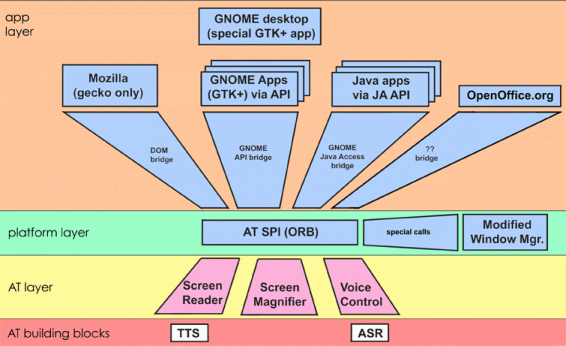
\includegraphics[width=1\textwidth]{obrazky-figures/GNOME_desktop_Accessibility.png}
	\caption{GNOME Accessibility Architecture overview\cite{gnomeADG}}
	\label{ATSPI_architecture}
\end{figure}

The widget is accessible, if a developer uses any GTK3/GNOME widget and follows the general accessibility guidelines\footnote{https://developer.gnome.org/accessibility-devel-guide/stable/gad-coding-guidelines.html.en} with properly implemented ATK interfaces. A newly developed widget, based on one of the stock GTK3/GNOME toolkit widgets, inherits the functionality and gains the accessibility support as well. The default implementation of the ATK interfaces might be altered by applications. Therefore, a developer can enrich their descriptions of widgets and improve the overall user experience in special cases, e.g. when a widget is used for some less expected purposes or the default description is too general. The ATK provides a set of functions to achieve this along with the ability to make any custom component accessible\footnote{https://developer.gnome.org/accessibility-devel-guide/stable/gad-custom.html.en}.\cite{accessibleWidgets}

\newpage
\section{Library Pyatspi}\label{library_pyatspi}
The package pyatspi is a Python wrapper around AT-SPI's C implementation, which loads the Accessibility typelib and imports the classes implementing AT-SPI interfaces.\cite{pyatspi}

AT-SPI exposes applications as a tree of widgets. On the top, the root element represents the whole GNOME desktop. Every sub-element represents one running application on the GNOME desktop. Each application has zero or more child elements, each child is distinguishable by its position in the tree and several object properties. Some of these properties are encapsulated inside the accessible object and their values must be obtained through corresponding methods, so-called \textit{getters}. A small set of properties are described in the following list:
\begin{itemize}
    \item \textit{name} - a string value, for most widgets contains text identical with a text label visible on a widget
    \item \textit{roleName} - a string value, specifies the widget type, available via \textit{getRoleName} method
    \item \textit{childCount} - an integer value, represents a number of sub-elements 
    \item \textit{actions} - a dictionary that contains available actions which can be performed on a widget by the ATK
    \item \textit{visible} - a boolean value, indicates that a widget is visible to the user
    \item \textit{showing} - a boolean value, a windget is rendered
    \item \textit{text} - a string value, mostly used in input fields or widgets containing plenty of text
    \item \textit{description} - a string value, contains a special widget description for users
    \item \textit{position} - an integer tuple, x, y coordinates on the screen (might be related to other component)
    \item \textit{size} - an integer tuple, shows the height and width of a widget
\end{itemize}

Additionally, the elements can be linked together in other useful ways (except the parent-child relationship), where the input widgets (e.g.: text field, check box, combo box, etc.) are linked with the elements that serve as their labels. These labels are making the input widgets easier to identify or interact with. Other advantageous element properties e.g. \textit{showing} or \textit{visible} are used to decide whether the element is hidden from the active screen area, thus it is not available for interaction. The \textit{roleName} attribute allows the categorization of widgets that is useful for identification of category-specific methods, e.g. selecting a radio button value, selecting an option in combo boxes, or a click method performed on push buttons. The access to the input functionality is focused in a singleton object named \textit{registry} that provides services for subscribing to specific events and generating  mouse or keyboard events on demand.

The library pyatspi is an open-source project available for most Linux distributions via distro specific packaging services (package named \texttt{python3-atspi}) or is available to be built from its sources\footnote{https://gitlab.gnome.org/GNOME/pyatspi2}.

\section{Exploring and Debugging The Accesibility}
Currently, there are several tools available for exploration and debugging accessibility features not only on the GNOME desktop.

\subsection{Dogtail}\label{sniff_accerciser}
Dogtail is an open-source GUI test framework written in Python and implemented as a library around the pyatspi. Several modules implement a higher level of API to simplify work and interaction with the accessible objects during the test development. The tool offers less complex functionality, containing tree view of objects with their basic attributes\cite{dogtail_doc}. 

The package dogtail also includes a GUI tool \textit{Sniff} (AT-SPI Browser on Figure \ref{sniff}), similar to the \textit{Accerciser} application described in the next section. The next paragraphs are dedicated to the description of the dogtail modules.

\begin{figure}[h]
	\centering
	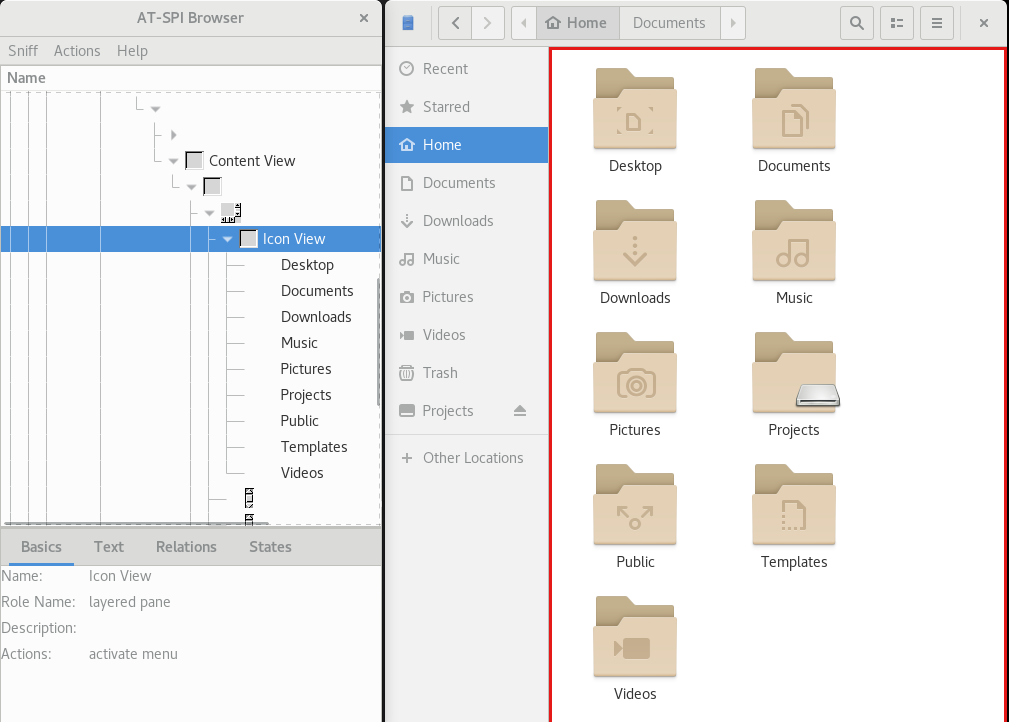
\includegraphics[width=0.9\textwidth]{obrazky-figures/sniff.png}
	\caption{Sniff utility (AT-SPI Browser), highlighting Icon View area in Nautilus File Manager, screenshot taken from Red Hat Enterprise Linux 8.2}
	\label{sniff}
\end{figure}

The module \texttt{tree} contains the most important class \texttt{Node}, instances of the class represent elements of the desktop user interface. All elements are gathered to the tree structure, representing all applications starting with the root element (desktop). The class is implemented as a mixin for Accessible and various Accessible interfaces and is an important unit for its subclasses, namely \texttt{Application}, \texttt{Root} and \texttt{Window}. The \texttt{Node} class also implements methods used for search of nodes in the tree based on certain criteria. A lambda expression can be passed to methods \texttt{findChild} and \texttt{findChildren} as argument named \texttt{pred}. The lambda expression can contain any properties that uniquely identify nodes, including \texttt{name}, \texttt{roleName},  \texttt{showing} and \texttt{visible}. The class also contains action methods that can be performed on nodes without importing other action modules. Verification and identification of shown nodes is easier thanks to the method named \texttt{blink}. Once the method is called on a certain element, the element is highlighted on the screen for several seconds. This functionality is also part of the Sniff tool where an element is highlighted after it is selected in the displayed tree.

The module \texttt{dump} contains only one method with the same name. The method returns a string describing the tree of nodes which is useful for python/ipython console debugging.

Finally, the module \texttt{rawinput} contains the implementation required for generating events from both keyboard and mouse. More complex events simulating keyboard shortcuts, mouse gestures, and drag and drop operations are implemented as well.

Testing Dogtail has proven availability for many Linux distributions through their package repositories, specifically Fedora 32, Red Hat Enterprise Linux 8.2 and Manjaro 18 with GNOME 3.34 (Archlinux). It is also available as a \textit{Pypi} Python package and according to information in it's official Gitlab repository should work not only for GTK3 application but also for application written in QT and KDE. 
 
Dogtail testing reveals some minor problems which might occur during the test development. There are known cases in which the coordinates of a node were not reported correctly. Most of the elements with the \texttt{roleName} value \textit{panel} and \textit{list box} are missing their \textit{name} values. Elements without the \texttt{name} value are much harder to identify, although they might not be important for users, as they don't contain any visible text, nor do they offer a way of interaction. The purpose of those elements is to serve as a wrapper that groups other elements together in a tree. 

Further testing discovered a non-accessible menu\footnote{https://bugzilla.redhat.com/1723836} or a nameless menu button\footnote{https://wiki.gnome.org/Apps/DiskUsageAnalyzer}. Once an action needs to be dispatched on such element, the identification has to be done either through a parent element or a sibling element. Additionally, the execution of a mouse event will require an offset calculation to specify the correct element position on the screen.
 
 So to conclude this chapter, dogtail is a powerful tool for the development of automated test cases in the GNOME3 environment. On the other hand, it contains discussed limitations and flaws. Those limitations must not come from the dogtail itself, they are either accessibility bugs or bugs in the GTK3 framework (non-accessible menu).  

\subsection{The Accerciser}
The Accerciser is an interactive accessibility explorer developed in Python. It provides a well-arranged graphical frontend for the AT-SPI library, hence it can inspect, examine and interact with widgets. It also serves as a verification tool for developers, to check that their applications are providing correct information to assistive technologies and automated testing frameworks. Compared to Sniff, Accerciser's interface (Figure \ref{Accerciser_img}) offers extended features and functions. The default interface has three sections, a~tree view with the entire hierarchy of accessible objects and two optional plugin areas. The~Accerciser has an extensible, plugin-based architecture. Most of the features available by default are provided by plugins discussed in the next several paragraphs.

The \textit{Interface Viewer} plugin is an explorer of the AT-SPI interfaces provided by each accessible widget of a target application. When a tree element is selected, its interfaces are shown with a list of sensitive methods. The majority of methods are executable. The list contains methods for interaction with an object and various methods for obtaining more information about the object. The Accerciser offers an exploration of the following interfaces:
\begin{itemize}
    \item Accessible - shows child count (number of child widgets), description, states, relations, and other attributes
    \item Application - if implemented (not mandatory), it shows application ID, toolkit and version
    \item Component - shows element's absolute position with respect to the desktop coordinate system, the relative position with respect to the  window coordinate system, size, layer type, MDI-Z-order indicating the stacking order of the component and alpha
    \item Document - shows document attributes and locale information
    \item Hypertext - shows a list with all element's hypertext links,  including name, URI, start index and end index
    \item Image - shows element's description, size, position and locale
    \item Selection - shows all selectable child items of the selected item,
    \item Streamable Content - shows selected element's content type and their corresponding URIs
    \item Table - shows element's caption, rows, columns, number of selected rows, number of selected columns and for the selected cell, it shows  it's row's and column's header extents  
    \item Text - shows selected element's text content, that can be editable with attributes offset, justification  and possibility to show CSS formatting as well
    \item Value - shows an element's value, minimum value, maximum value, minimal increment for a value 
\end{itemize}

\begin{figure}[hbt]
	\centering
	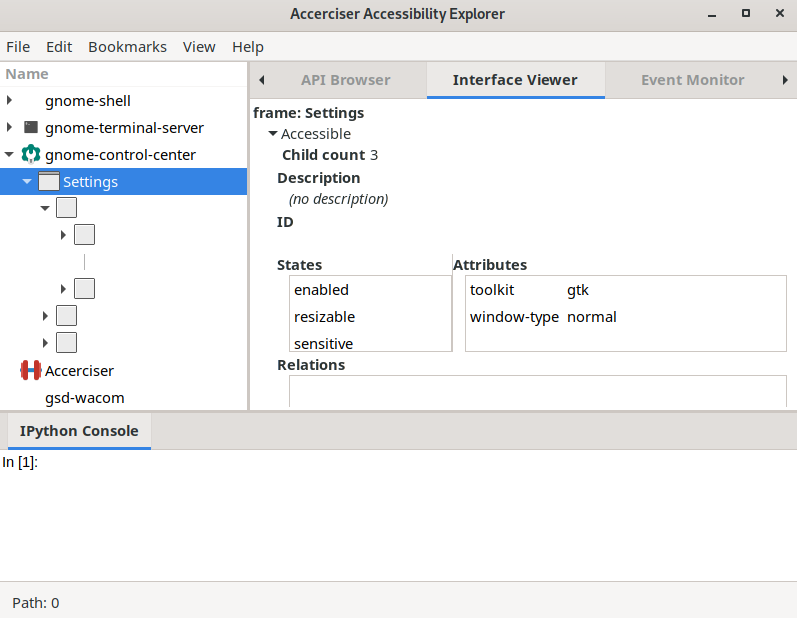
\includegraphics[width=0.9\textwidth]{obrazky-figures/accerciser.png}
	\caption{Accerciser's default configuration, Screenshot taken on Manjaro Linux with GNOME 3.34}
	\label{Accerciser_img}
\end{figure}

The \textit{AT-SPI Validator} plugin applies tests to verify the accessibility of a target application. The validator will generate the report of the selected item and all its descendant widgets in the tree hierarchy.

The next plugin is the \textit{Event Monitor}, which displays AT-SPI emitted events including the filter for several different AT-SPI event classes. The plugin has the ability to monitor only events sourced from the selected application or a selected accessible (widget). Each event record contains the source and the application.

The \textit{Quick Select} plugin provides global hotkeys for quickly selecting accessible widgets in the Accerciser's Application Tree View, the selected widget is highlighted in the target application.

The \textit{API Browser} plugin shows interfaces, methods and attributes available on each accessible widgets of a target application. By default, it shows only public methods and properties. Private methods and properties are hidden until checkbox \textit{Hide Private Attributes} is unchecked.
 
Finally, the plugin \textit{IPython Console} provides a full, interactive Python shell. The console has immediate access to any selected accessible widgets of a target application. The currently selected object in the tree view is available in the IPython Console under the symbol \textit{acc}. The plugin provides an easy way to test and debug code used in test cases.    
\section{Covering Limitations of Accessibility and Verification}
As discussed in the aforementioned sections, the information provided by accessibility is not flawless. Therefore, the next couple of chapters are dedicated to the exploration of technologies that might be used to support the accessibility in such cases.

\subsection{OpenCV and Image Matching Techniques}
OpenCV or Open Source Computer Vision Library is a software library that provides optimized algorithms for computer vision and machine learning. According to the official OpenCV webpage\cite{opencv}, the library contains more than 2500 algorithms and it is being developed 
by a vast community of contributors around the world. The library is used extensively bu government institutions, research groups, and companies including Microsoft, Google, IBM, etc. One of the biggest advantages is its native C++ implementation with bindings making the library available in Python, Java, and Matlab and supports Linux, Android, Mac OSX, and Windows. Regardless of Linux distribution, similarly to dogtail, OpenCV can be installed easily via python3 package manager (\texttt{pip}). 

From the rich availability of algorithms provided, the image recognition algorithm can be used to either locate or verify the presence of an element on the screen. This approach would require to have a set of images containing elements prepared in advance, then it can be used to find the image location on the screenshot of the screen taken during a test run. Compared to verification of the node only via accessibility, this approach would also verify that the element is properly rendering on screen and the shown result is an element that is shown to the user. An additional benefit is the verification of text formatting and colors. On the contrary, this process requires additional manual work of taking images, labeling them, and associating them with certain test scenarios. Count of elements displayed on the screen multiple times creates another parameter that would require manual maintenance. The most common example of such cases are buttons labeled either OK or Cancel as they are used in many applications.

Another possible approach is to use the shape recognition algorithm which can locate shapes like circles, rectangles, and many other common shapes. From the development perspective this would be easier to maintain, as there is no requirement for images prepared in advance. Frequent application changes during software development may also cause that tests based on image matching can be easily outdated. This factor forces testers to revisit test suites, therefore the efficiency of automated tests deteriorates. It can also help with the widget location in cases where accessibility is reporting wrong coordinates. On the other hand, locating the right widget in cases when several similarly shaped ones are located on the screen at the same time will yield very inconsistent results.

\subsection{OCR}\label{OCR_section}
The Optical Character Recognition or OCR is a method of extracting text from images. One of the available open-source tools is a tool called Tesseract.

Initially, Tesseract development started in 1985 at Hewlett Packard Laboratories but the major breakthrough was achieved in 2006 when the project was open-sourced in cooperation with the University of Nevada in Las Vegas. Since then, the project has been developed under the sponsorship of Google\cite{tesseract_history}.

Usability of Tesseract was increased in version 3.x, supporting a wide range of image formats and gaining the ability to be used in a larger number of scripting languages. While Tesseract 3.x is based on traditional computer vision algorithms, in the past few years methods based on Deep Learning have surpassed traditional machine learning techniques by a vast margin, especially in terms of accuracy in several areas of Computer Vision. Remarkable results were achieved in handwriting recognition. Tesseract has implemented a Long Short Term Memory (LTSM) based recognition engine which is a kind of Recurrent Neural Network (RNN). While this kind of RNN is used to recognize the text of random length, a Convolutional Neural Network is used just for recognition of single character. Version 4 provides both legacy OCR engine and new LSTM engine which is enabled by default.\cite{tesseract}

Tesseract can be used as a command-line tool, integration in development is possible via Tesseract's API available in python or C++. Setup on Linux or other platforms may differ but the process is accurately described in Tesseract's wiki\footnote{https://github.com/tesseract-ocr/tesseract/wiki}, with the last resort solution - building it from its sources.
The setup process includes installation of the \texttt{tesseract-ocr} package itself, \texttt{pytesseract} python bindings installable via python's package manager pip, and Tesseract's language pack with trained data for English language (version 4.x supports 130 languages\footnote{https://github.com/tesseract-ocr/tesseract/wiki/Data-Files\#data-files-for-version-400-november-29-2016}). 

Tesseract's OCR engine works best when used with images containing black text on white background in a common font. Text should be approximately horizontal with the height of at least 20 pixels. Surrounding borders around the text can be detected as some random text. With possibilities of image processing provided by OpenCV, the image quality in some cases needs to be improved before applying text detection methods. The most common image preprocessing methods include inverting images, rescaling, binarisation, noise removal, rotation, border removal, and page segmentation\footnote{https://github.com/tesseract-ocr/tesseract/wiki/ImproveQuality}.

Tesseract's API for python is bundled in a module named \texttt{pytesseract}. The module provides several methods, the most important ones for the purpose of this work are \verb|image_to_string| and \verb|image_to_data|. Both methods have one compulsory parameter which is an image intended for text extraction. An image has to be in a certain format, one of the options is to load the image through OpenCV's \texttt{imread} method. Additional parameters may be applied including language, timeout, and engine configuration\footnote{https://pypi.org/project/pytesseract/}. The first method returns all recognized strings including all whitespaces and other special characters. The second method provides additional metadata about all recognized strings in a form of dictionary-like object. The returned dictionary contains the following lists of properties:

\begin{itemize}
    \item text - string value, may contain a string, special character, one word or line of text
    \item left - integer value, specifies the number of pixels from the left side of the image 
    \item top - integer value, specifies the number of pixels from the top of the image
    \item width - integer value, specifies the width of the recognized string 
    \item height - integer value, specifies the height of the recognized string
    \item the rest are less important values for this work: \verb|level, page_num, block_num par_num|
    \verb| line_num, word_num, conf|
\end{itemize}

\begin{figure}[H]
	\centering
	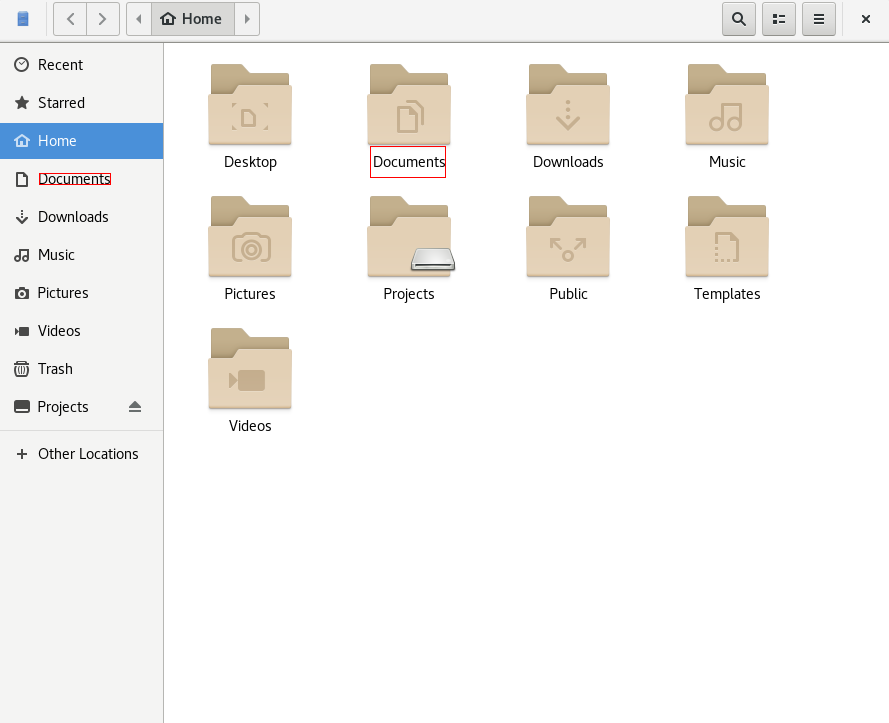
\includegraphics[width=0.9\textwidth]{obrazky-figures/ocr+nautilus.png}
	\caption{Demonstration of the OCR engine detection for the string Documents in Nautilus File Manager window, Red Hat Enterprise Linux 8.2}
	\label{ocr_nautilus}
\end{figure}

Figure \ref{ocr_nautilus} contains a demonstration of the Tesseract engine capabilities. The task was to locate the string \textit{Documents} in the screenshot of the GNOME file manager application \textit{Nautilus}.
The engine successfully found both strings located in the image and provided coordinates and dimensions that were used by OpenCV to highlight the strings in the image. 

Similarly to OpenCV, Tesseract's OCR engine was tested as an alternative tool for location or verification of widgets that contain text. This method also verifies that the content was properly rendered and is readable for the user. OCR systems have limitations and work with a certain margin of error which is a fact that also applies to Tesseract. Various applications can use different color schemes including background colors and font colors, input fields, and labels. Highlighting elements to perform actions on them can also lead to changes in color conditions. Image preprocessing methods provided by OpenCV can aid in avoiding problems associated with those cases, namely color inversion and binarisation. Those methods would supply Tesseract's engine with an image containing black text and a white background for evaluation.

\section{Conclusion}\label{ocr_conclusion}
This chapter has been dedicated to the Accessibility technologies in GNOME desktop with a deeper look at implementation, libraries, and tools for debugging. Furthermore, technologies that may be able to cover limitations and bugs in accessibility have been evaluated as well. Both OpenCV and Tesseract may help with identification, location, and verification of non-accessible elements in applications. A possible disadvantage is a delay caused by taking and processing screenshots of applications that have to be taken at the right time. OpenCV's image matching algorithm can reliably locate prearranged images of icons, labels, or whole application windows on the screen. Considering the stable application environment with black text on white background in most applications, Tesseract can detect and reliably locate most of the text content on the screen. Other cases can be covered by image preprocessing done again in OpenCV. Both technologies are working with actual application content rendered to users, possibly bringing an additional level of verification. However, the goal of this work is to generate test cases dynamically and preparation of a set of screenshots to verify a proper rendering of icons would violate this effort. A possible solution could be to take screenshots during the test generation process. However, an icon would need to be cropped out from the screenshot, thus relying on the position if the icon reported by the AT-SPI. Therefore, an integration of the Tesseract's OCR would be more beneficial for this project.

\chapter{Proposed solution}\label{proposed_solution}
A goal of this work is the development of a tool with the ability to generate automated test cases for GUI applications. The proposed test generator works with the AT-SPI metadata provided by applications and converts them to test cases. The required metadata should be available for a lot of applications, assuming they are developed in one of the common frameworks (GTK3, QT). However, this tool is focused on applications for GNOME desktop\footnote{https://wiki.gnome.org/Apps}. A tool will be developed in language Python3, version 3.6.

All applications are open source and are developed by the community of enthusiasts around the GNOME project. Anyone from the community can fix bugs in applications by sending a merge request with fixes, request a new feature, or propose newly developed features. This development model does not contain a planning phase or a phase where one can design an abstract model of an application, from which test cases could be derived. Therefore, the solution is based on the derivation of the model from the AT-SPI metadata. The extracted data about widgets and relationships between them, provides the foundation which gives the test generator the ability to interact with an application. Therefore, the test generator can use the extracted information to perform the exploratory testing. The testing includes execution of the scenarios (or so-called \textit{test sequences}), monitoring the behavior of the SUT, and detection of certain errors and crashes of the SUT. The test cases are generated as a by-product of this process.

\begin{figure}[hbt]
	\centering
	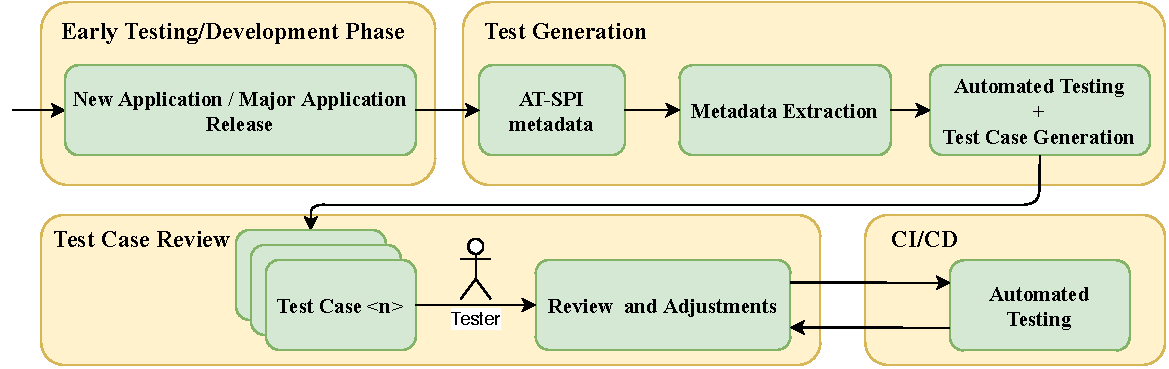
\includegraphics[width=1\textwidth]{obrazky-figures/overview.pdf}
	\caption{Architecture of the proposed solution}
	\label{Diagram}
\end{figure}

Figure 4.1 describes an overview of the workflow with the proposed test generator. The beginning of the scenario starts with either a newly developed application or a version of an application that contains major changes. The tool should perform initial exploratory testing of the application based on the extracted model and export those scenarios in the form of \textit{behave} test scenarios.

From the testing perspective the proposed tool combines several testing techniques. The extracted AT-SPI metadata creates the foundation for a simplified model of the application by partially adapting the model-based testing technique. Since the test cases are derived from the model without any knowledge about the implementation of a tested application, the tool resides in the category of black-box testing. The knowledge about the SUT provided by the model allows the tool to benefit from the approaches described in the random input testing and random walk tools in a more deterministic way. The tool can be characterized as a semi-smart tool as it can detect certain crashes of the SUT during the test generation and immediately report them with a reproducer. The results of the test generation process are test cases that may be adjusted and executed again. The tests are executable in the CI/CD pipeline that can be triggered at any stage of the application development and report the results without manual retesting.

\section{Model Extraction}
The model extraction process relies on the AT-SPI metadata that are provided after the start of an application. As mentioned in section \ref{library_pyatspi}, once the application is running, a tree of widgets is exposed and available for interaction. The provided representation of the tree itself is not suitable to be directly used as a model of an application, as the implementation contains several restrictions for purposes of this work.

The first restriction is represented by nodes/widgets with no functionality nor a way of interaction for the user, e.g.: filler, separator, panel, etc. Theoretically, a copy of the three could be created with those nodes filtered out, although in that case the parent-child relationship in the tree needs to be restored accordingly. This is not possible, since the attributes \texttt{children} and \texttt{parent} in \texttt{Atspi.Accessible} object instances are read-only. The tree also contains references to properties and methods which are available only during application runtime and possibly disallowing access to the properties of an extracted model after application crashes or terminates. Furthermore, the test generator must start the execution of every test scenario (test sequence) from the default state which is achieved by obtaining a fresh instance of a tested application.

A solution for those restrictions is a custom implementation of the accessibility tree. In the beginning, a custom tree is derived from the original tree provided by the \textit{dogtail}. The unusable nodes are filtered out, while the parent-child relationships of the nodes are preserved. The custom tree can be used as a model, that will map the possibilities of interactions available for users working with an application. The model includes every node from the original tree with available actions that are also executable by the AT-SPI. 

However, the model does not allow the execution of the actions directly, as the generation process requires to run several instances of an application. The instances of accessible objects and some of their properties are valid only for one application runtime. Therefore, several important values are extracted in the process, making them available even after the termination of an application instance. The properties \texttt{name, roleName, parent\_name, parent\_roleName} are used as the unique identifier because some nodes might share the same \texttt{name} and \texttt{roleName} (e.g. OK, push button). The properties give the test generator the ability to match each node from the model to the current application instance exposed by the accessibility. The implementation of the model is presented in the class diagram in Figure \ref{tree_diagram}.

\begin{figure}[hbt]
	\centering
	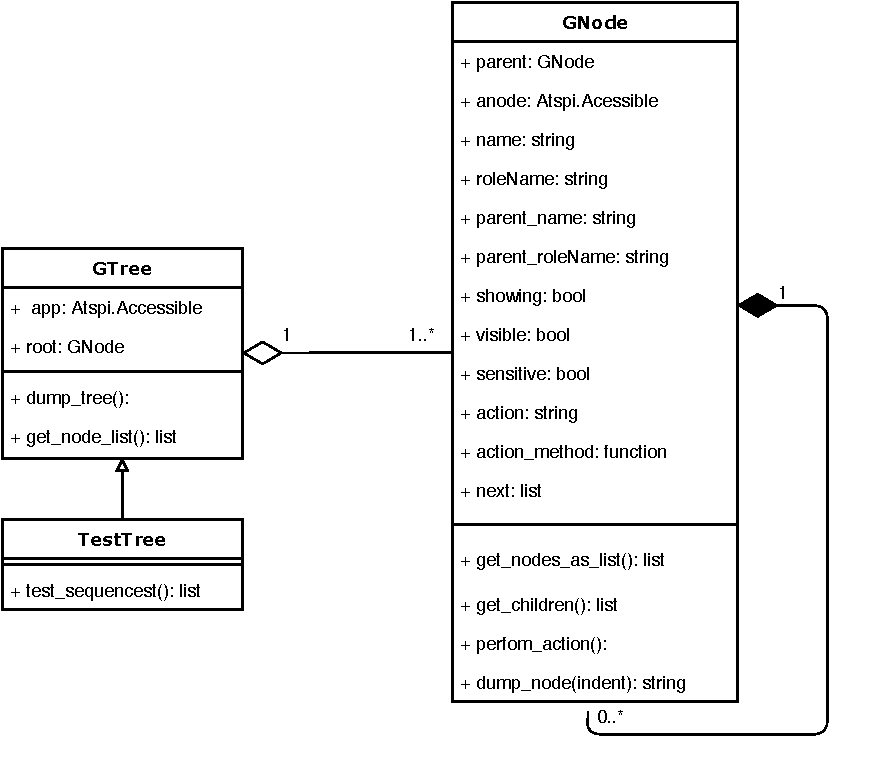
\includegraphics[width=0.8\textwidth,clip]{obrazky-figures/tree_diagram.pdf}
	\caption{Class diagram of the model}
	\label{tree_diagram}
\end{figure}

Starting from the lowest level, an instance of the class \texttt{GNode} represents one node from the tree. Several attributes are copied from the original \texttt{dogtail.tree.Node} instance, including attributes storing the pieces of information about the parent node, the data describing the state of the node, the list of children, and if available, the name of the action method. The list of children is also composed by instances of the \texttt{GNode} class, so the tree is recreated recursively. Therefore, the model is able to hold all information about tested applications, without relying on their state. An instance of the \texttt{GTree} can represent either a whole application or a smaller part of the application e.g.: a dialog or a menu. As discussed previously, this offline model of the application tree also contains a lot of nodes without the ability of interaction, which needs to be filtered out. Those nodes are identified by the list of \texttt{RoleName}s that are gathered in the separate file \texttt{rolenames.py}. Finally, the class \texttt{TestTree} serves as a wrapper that filters those nodes and preserves the parent-child relationship. The result of this process is an instance of the \texttt{TestTree} object and it contains only nodes required to generate test cases. 

\newpage
\section{Test Environment}
Before the generation process starts, it is necessary to have the implementation for monitoring the state of tested applications and acquire the ability to perform start and stop operations. The test generation process performs various actions available in an application that might change settings or layout of the application. Generation of every test case must start from the same state which should satisfy the following conditions: 
\begin{enumerate}
    \item an application is not running, if so, force the application to stop
    \item reset the application's settings to default state by performing predefined custom cleanup
    \item start a new instance of the application with the default settings.
\end{enumerate}

\subsection{Test Environment Setup}
The test case generation process depends on the execution of applications in GNOME Shell desktop environment. The environment contains various features\footnote{\url{https://help.gnome.org/users/gnome-help/stable/shell-introduction.html.en}} like workspaces, notifications, the application grid, the activities overview, and menus, that can be triggered either via mouse or keyboard. Those actions can bring the environment to multiple states. Execution of an action that brings the environment to some of those states takes the focus from the tested application back to GNOME Shell, thus blocking any further interaction. A notification might collide with the user interface of the tested application and block the execution of an action during the test case. These factors need to be avoided to ensure stability during the test generation and the test execution as well. The setup must also be able to recover the environment from potential test case failures and will not influence the execution of the subsequent test cases. 

The required setup for the test execution is implemented in the module \textit{qecore}. The module is designed for test automation of GNOME desktop applications and contains various measures designed to avoid occurrences of unintentional environment events and focus on a tested application. The module is bound to \textit{dogtail} and it is intended to be used with \textit{behave} framework.\cite{qecore} 

The test generation process partially relies on the provided setup. However, a different approach is used in terms of monitoring tested applications. For this reason, a custom class \texttt{App} is derived from the qecore's \texttt{Application} class. Throughout the development of the test generator, the implementation of the \texttt{App} class diverged, and the majority of the implemented methods were rewritten. Although, the \textit{qecore's} \texttt{Application} class is still being used for the test case execution. The inheritance acts as a safeguard that makes sure that provided data about tested applications are sufficient to create an \texttt{Application} instance. Or in other words, it serves as an assertion that generated tests will be executable before the generation process starts. The relationship between classes is shown in Figure \ref{test_gen}. The test generator integration with the \textit{qecore} lead to contributions that were delivering minor fixes\footnote{\url{https://gitlab.com/dogtail/qecore/-/merge_requests/24}}\textsuperscript{,}\footnote{\url{https://gitlab.com/dogtail/qecore/-/merge_requests/26}}. Another contribution\footnote{\url{https://gitlab.com/dogtail/qecore/-/merge_requests/25}} submitted an implementation of the new attributes for the \texttt{Application} class to solve the problem with location of desktop files required to test LibreOffice applications.

\subsection{Test Environment Configuration}\label{env_config}
Assurance of compatibility with various applications across the GNOME ecosystem requires that some metadata describing the tested application has to be provided before the test generation process. The metadata is gathered in a configuration file written in YAML\footnote{\url{https://yaml.org/}} language and only contains the most necessary information required to recognize tested applications. The reasons behind choosing YAML is syntax simplicity and human readability in comparison with e.g. JSON\footnote{\url{https://www.json.org/json-en.html}} or XML\footnote{\url{https://www.w3.org/XML/}}, followed by the reliable support in Python provided by library \texttt{pyyaml}.\cite{yaml} The  configuration file serves as a single source of truth for the test generator. All changes in the medatada required to test the application are done within this file, thus avoiding any changes in the source code of the test generator.

\begin{lstlisting}[language=yaml,caption={Example of the apps.yaml entry for LibreOffice Start Center},label={apps.yaml}]
libreoffice-startcenter:
  a11y_app_name: soffice
  app_process_name: soffice.bin
  desktop_file_path: /usr/share/applications/libreoffice-startcenter.desktop
  kill_command: "pkill soffice"
  params: "--norestore" # required to avoid unwanted file restore dialogs
  cleanup_cmds:
    - "pkill soffice" # LO required a custom kill cmd
    - "rm -rf .config/libreoffice/*"
  packages:
    - libreoffice
  flatpak: False
\end{lstlisting}

The \texttt{apps.yaml} gathers data about all tested applications. Each application entry starts with an application name on the top level. The application name should be unique as the name is used as a folder name of the generated project. Required values may vary per tested application. Some of them might not be necessary for the test generation, although they are required for the test execution.
The list of items that can be defined for each application includes:

\begin{itemize}
    \item \texttt{a11y\_app\_name} - is the only compulsory item, it defines a name of the application in the accessibility tree, the value can be found in GUI tools Sniff or Accerciser as previously discussed in Section \ref{sniff_accerciser}, the value can match with the name of the application
     \item \texttt{app\_process\_name} - is required if the name of the application process differs from the application name, the value is used during the cleanup in between the executions to make sure that an instance of the application has been killed and a next test will use a new one
     \item \texttt{desktop\_file\_path} - required if default qecore's method fails to find the desktop file of an application, the desktop file contains useful data about applications, including a command required to run an application from the command line
     \item \texttt{params} - required if the application needs to be run with custom command line parameters, all parameters should be entered in one string, separated with a space
     \item \texttt{cleanup\_cmds} - if provided, contains a list of commands that will be executed after the generation of each test case. Executed commands should always restore the application to its default settings. The commands are also used during the test execution of generated test cases, after finishing each test case. 
     \item \texttt{packages} - required for execution in the CI environment, contains a list of rpm\footnote{https://rpm.org/} packages required to be installed to both generate and execute tests
     \item \texttt{flatpak} - required if a tested application is a flatpak
\end{itemize}

\subsection{Flatpak Applications Setup}
Flatpak\footnote{\url{https://flatpak.org/}} is a technology for building and distributing desktop applications on Linux. Flatpak aims to solve the problem with the cross-platform distribution of packages on Linux, thus avoiding problems with different package managers used across Linux distributions. Applications, or so-called flatpaks, are delivered to users regardless of the lifecycle of the underlying Linux distribution. The system implements a set of sandboxing technologies, to isolate flatpaks from each other and the system, thus providing security benefits to users.\cite{flatpak}

The majority of GNOME applications are also available through flatpak. A dedicated flatpak repository \textit{Nightly GNOME Apps} contains the latest development versions of GNOME applications. With Flatpak, those applications are installed alongside their stable versions. This gives us the potential to test the application much sooner before it is released to distributions. This is a benefit behind the integration of flatpak support to this work. The main repository for flatpak applications called Flathub\footnote{\url{https://flathub.org/home}} contains hundreds of applications developed in various frameworks and programming languages. However, the effort done by this work only supports applications developed in GTK3 as they obtain the accessibility support by design.

There are several differences in the runtime perspective between flatpaks and non-flatpak applications. Each application has a unique name, e.g.: \texttt{org.gnome.gedit}. The unique name is required for every operation executable through the \texttt{flatpak} command-line utility. The utility not only serves as a package manager able to install, remove, downgrade and update flatpaks, it also provides a sandbox to run flatpaks. Those differences demand certain changes in the runtime used for the test execution and the test generation. 

Considering the test execution, the approach used in the \textit{qecore's} \texttt{Application} class should be suitable for testing flatpaks. However, the initial testing emphasized the previously mentioned differences and it lead to the conclusion that a separate class \texttt{Flatpak} has to be developed to achieve the same goals. The \texttt{Flatpak} class inherits the methods from the \texttt{Application} class and reimplements some of them do address those differences. The most important changes are:

\begin{itemize} 
    \item \texttt{\_\_init\_\_} - the constructor performs a validity check on inserted flatpak ID, the format requires two dots, e.g. \texttt{org.gnome.gedit}
    \item \texttt{start\_via\_command} - runs a flatpak via only via command and with the flatpak command-line utility, e.g. \texttt{flatpak run <id>}
    \item \texttt{kill\_application} - terminates a flatpak via command e.g. \texttt{flatpak kill <id>}
    \item \texttt{get\_desktop\_file\_path} - performs a recursive search for flatpak's \texttt{.desktop} file in two possible locations:
    \begin{itemize}
        \item \texttt{\textasciitilde/.local/share/flatpak/app/} - flatpak installed per-user
        \item \texttt{/var/lib/flatpak/app/} - flatpak installed system-wide
    \end{itemize} 
    \item \texttt{is\_running} - performs a check if a flatpak is running, this is again done with the flatpak command-line utility (e.g. \texttt{flatpak ps <id>}) and the presence of an instance in the accessibility tree
\end{itemize}

Additionally, the invocation of some of the inherited methods does not make sense for flatpak applications. The invocation of those methods with an instance of the \texttt{Flatpak} class raises an exception. The exception contains a message with an explanation that the methods are not available for Flatpak objects. The developed changes were submitted to the \textit{qecore} projekt{\footnote{\url{https://gitlab.com/dogtail/qecore/-/blob/master/qecore/flatpak.py}}}.

On the test generator level, a new class \texttt{FlatpakApp} was implemented to manage the runtime of the flatpak applications. As described in the class diagram shown in Figure \ref{test_gen}, the \texttt{FlatpakApp} serves as a wrapper for the \texttt{Flatpak} class in the same manner as the \texttt{App} class wraps the \texttt{Application} class. \texttt{FlatpakApp} and \texttt{App} are customized classes for the test generator, while \texttt{Flatpak} and \texttt{Application} are used during the text execution. 

\subsection{Monitoring an Application State}
There are several indicators that can be monitored while the application is being tested. The most essential one is to be able to safely determine if the application is running at the moment or not. This can be done either by examination of the \textit{pid} (process id) belonging to the application process or by relying on AT-SPI. If the application tree is not available, it can be certainly assumed that the application instance is not running. This statement also applies vice versa, so an assertion that an application has started is achievable in the same way. The implementation takes advantage of \textit{dogtail's} \texttt{Tree.Node.Applications()} call, returning a list of applications currently exposed to the accessibility bus.

Furthermore, it is also necessary to perform certain checks during the time an application is being interacted with. Therefore, every tested application will be run as a sub-process, which enables us to capture the output generated by tested applications to standard streams (\textit{stdout, stderr}). Once an application has been terminated, it also allows us to check the return codes. The implementation relies on Python's standard library \texttt{subprocess}. 

The output generated to the standard stream is checked for errors defined in the designated configuration file. In case of error throughout the generation process, an error message is printed immediately to warn about the possible bug in tested applications. The warning contains the number identifying the test in which the error occurred, a full error message, and a return code. All other captured messages e.g. warnings or deprecation messages from the GTK framework are saved to one log file, in a folder where the tests are generated. The messages are being appended, so the log file can be checked at any time during the generation process. Every line contains the test number, so it can be easily determined when the message occurred and match it with the reproducer from the given test case.

The implementation for the non-flatpak applications is encapsulated in the class \texttt{App}. The class \texttt{FlatpakApp} achieves the same goals for the flatpak applications.

\begin{figure}[H]
	\centering
	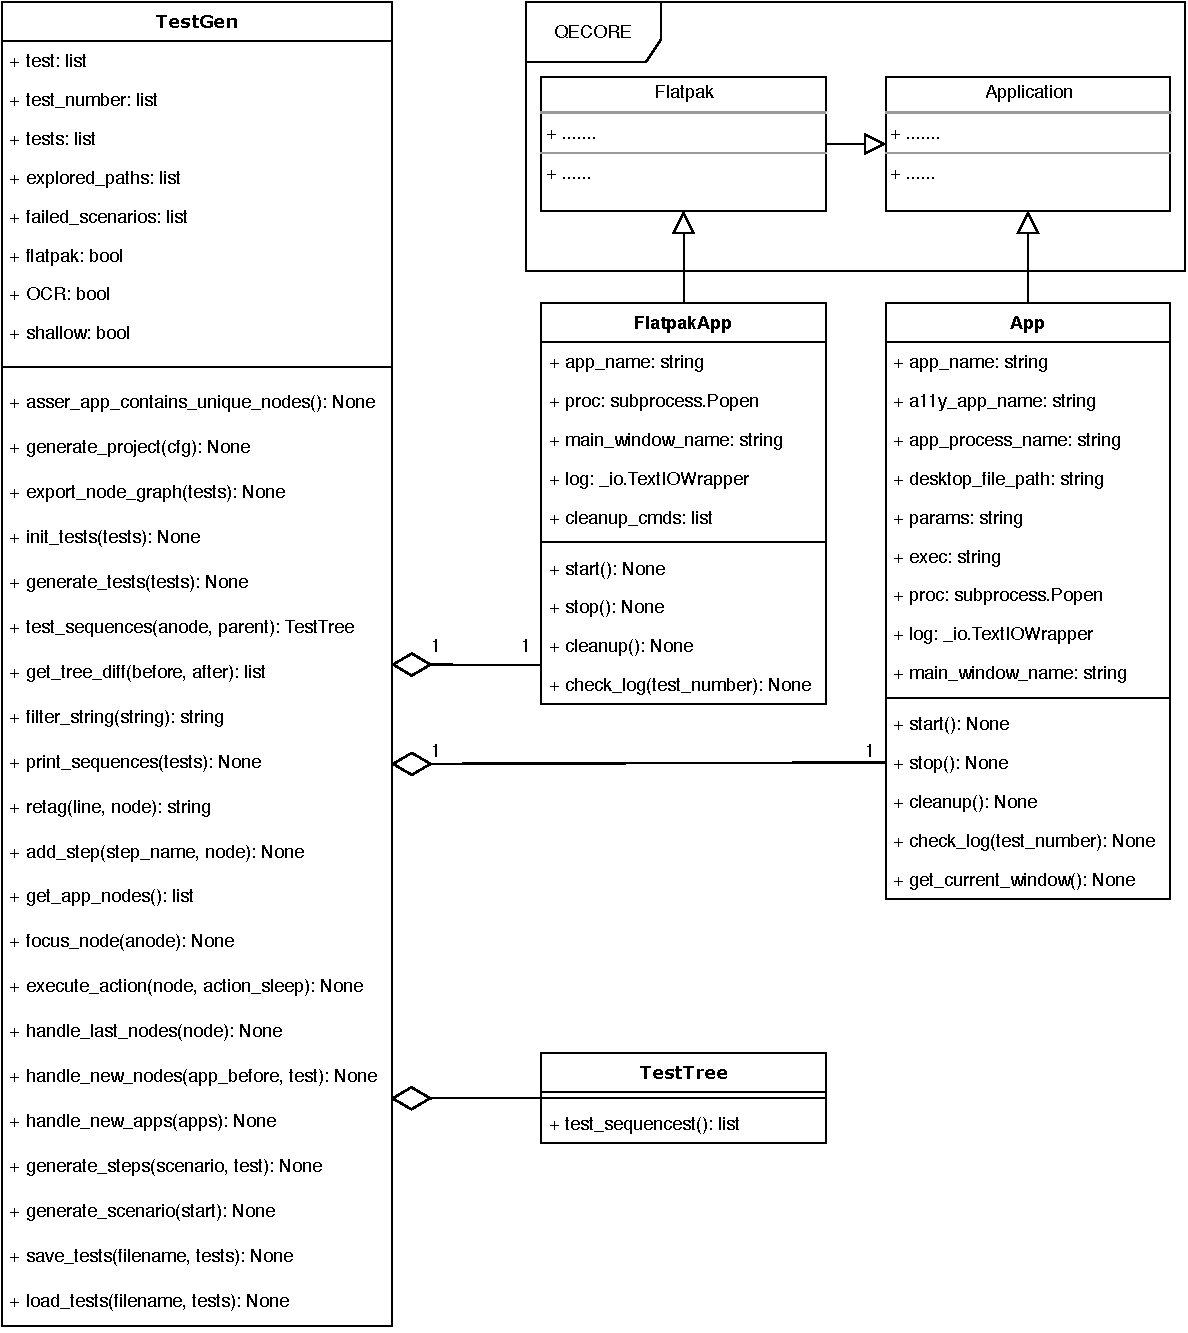
\includegraphics[width=1\textwidth,clip]{obrazky-figures/TestGen_class_diagram.pdf}
	\caption{Class diagram describing an overview over the implementation of the test generator}
	\label{test_gen}
\end{figure}

\section{Generating Environment for the Test Execution}
The input of test generator is provided by the data in \texttt{apps.yaml}. The output is a project structure containing generated test cases and other files required for the test execution. 

Initially, the test generator checks the availability of the entry for a tested application in the configuration file \texttt{apps.yaml}. Subsequently, it creates a sub-folder with the name of the application where generated content will be placed. Predefined source files with the implementation of \textit{steps} (used by \textit{behave} framework) are copied to the folder structure along with scripts and other files that are necessary for the test execution. Figure \ref{project_folder} demonstrates the structure generated for the application \textit{GNOME Terminal}.

\begin{figure}[H]
\dirtree{%
.1 gnome-terminal.
.2 features.
.3 generated.feature.
.3 environment.py.
.3 steps.
.4 ocr\_steps.py.
.4 steps.py.
.2 gnome-terminal.log.
.2 mapper.yaml.
.2 requirements.txt.
.2 runtesh.sh.
.2 cleanup.sh.
}
\caption{The generated project structure for the application \textit{GNOME Terminal}}
\label{project_folder}
\end{figure}

The sub-folder named \texttt{features} contains files with the \textit{behave} test cases. Test cases generated by the test generator are in the file \texttt{generated.feature}. The file contains a single so-called \textit{Feature} that contains all generated test cases. Test cases are composed of a tag, a brief description of the test case, and so-called \textit{steps}. The tag is a unique identifier of the test case and thus allows single test case execution, if required. The description should briefly define what should be done with the SUT, when the test case is executed. The steps are one-line statements, each of them describes either an execution of an action or an assertion described in a human-readable language. Successful execution of all steps evaluates the test case as passed. Otherwise, the result of the test case is a fail.

The file \texttt{environment.py} contains the setup required for the test execution. It contains 3 functions used by the \textit{behave} framework to set up or restore the required environment during the test execution. 

The \texttt{before\_all} function is run once before the execution of the test cases. It initiates the GNOME environment setup from the \textit{qecore} library and creates an instance of either the \texttt{Flatpak} or the \texttt{Application} class. The type of the application and the parameters for the class instance are extracted from the entry in the configuration file \texttt{apps.yaml}. 

The \texttt{before\_scenario} function is executed before every test case (scenario). It contains an invocation of the method from the \textit{qecore} that should set the testing environment to the default state and other preparations for the testing. Additionally, it executes the \texttt{cleanup.sh} script with a custom per-application cleanup defined in \texttt{apps.yaml} (discussed in Section \ref{env_config}). 

The \texttt{after\_scenario} function is called after the execution of every test case, regardless of its results. The result is then submitted to the generated test report.

The folder \texttt{steps} contains source files with the implementation of the \textit{steps} used in the \textit{behave} scenarios. The implementation of steps is divided into two files. The module \texttt{ocr\_steps.py} contains only one \textit{behave} step which encapsulates the implementation and optimization used for the verification of the string on the screen. The module \texttt{steps.py} contains general implementation of steps. The steps are functions implemented in Python with the \texttt{step} decorator from the \textit{behave} framework. The decorators serve as a wrapper to call the Python functions from the \texttt{.feature} files. So in the case of this project, the steps written in the test cases are function calls, the functions are defined in these modules. The definition of the \texttt{@step} decorator (Code Listing \ref{step_definition}) contains variables, thus allowing us to keep the code base as minimal as possible.

\begin{lstlisting}[
style=mypython,
caption={The implementation of the step that is used to make an assertion on any of the node's property},
label={step_definition},
  frame=tb,
  numbers=left
]
@step('State: "{roleName}" "{name}" "{prop}" is "{state}"')
def assert_state(ctx, name, roleName, prop, state):
    node = ctx.app.instance.child(name, roleName)
    focus_node(node)
    assert hasattr(node, prop), f'Obj: {node} is missing attribute {prop}'
    prop_value = f'{getattr(node, prop)}'
    assert state == prop_value, f'Expected: {state}, Got: {prop_value}'
\end{lstlisting}

The file \texttt{gnome-terminal.log} aggregates log messages produced by a tested application throughout the test generation process. The log file name is derived from the application name defined in the \texttt{apps.yaml} file. The \texttt{mapper.yaml} file contains a list of test cases with other data required for the CI execution. The file \texttt{requirements.py} contains all Python dependencies that need to be installed to execute the test cases. Finally, the \texttt{runtest.sh} is a wrapper script for execution of test cases.

\section{Test Case Generation}
The test generator implementation is encapsulated in the class \texttt{TestGen} (class diagram in Figure \ref{test_gen}). The behavior of the generator can be also influenced by several command-line arguments that will be described later in this work. Based on the parameters (\texttt{flatpak} item in \texttt{apps.yaml}), the instance of either the \texttt{App} or the \texttt{FlatpakApp} is created. 

The generator then creates a copy of the default project structure and injects the files inside the project structure with values that correspond to the application that is going to be tested (Figure \ref{project_folder}). Namely, the files \texttt{environment.py}, \texttt{mapper.yaml}, and \texttt{cleanup.sh} contain placeholders (tags) that are replaced by values defined in \texttt{apps.yaml}. Just note that no Python code is being generated during the process. The default project already contains all the predefined \textit{behave} steps required to execute generated test cases.
The next sections are dedicated to the details of the generation algorithm. The Algorithm \ref{test_gen_algorithm} contains a shorter version written in a pseudocode. 

% duplicit node renaming
\subsection{Derivation of Test Sequences}

The generator proceeds with a first start of a tested application and extracts the AT-SPI tree of the application instance through the \texttt{dogtail}. Then, a writable copy of the tree is created through the \texttt{GTree} instance. The action-less nodes are then removed and the remaining notes are placed in the new instance of the \texttt{TestTree} class. Test cases are derived from the test tree through the class method \texttt{test\_sequences}. 

The method returns a list\footnote{\url{https://docs.python.org/3/tutorial/datastructures.html}} with test sequences. A test sequence contains a list of nodes with actions that will be executed for every test case. The method gathers the list of leaves in the \texttt{TestTree}. Then it iterates through the list of leaves and calculates path from a leaf to the root of the tree. Each path contains a list of nodes. The result is a list of paths or as mentioned earlier test sequences. A test sequence does not represent a whole test case. The whole test case is created by applying the test sequence on the live instance of the application. While applying the test sequence, the generator appends assertions steps and OCR checks. The checks are generated either before or after the execution of actions and they will be used as a verification in a generated test case to confirm that the application reached the intended state. A test sequence can be used multiple times or it can be extended, if the generator discovers that the applied sequence leads to a discovery of new nodes. Those new nodes are evaluated and the generator creates new test sequences, each of those sequences start with a sequence that leads to their discovery. 


\begin{center}
\begin{algorithm}[H]
\caption{Test generation algorithm pseudocode}
\label{test_gen_algorithm}
\SetAlgoLined
\KwData{Running application exposed to the accessibility bus, \texttt{apps.yaml}}
\KwResult{Test Cases}
 start the application\;
 scan the application tree, generate the test tree\;
 derive the test sequences\;
 terminate the application\;
\SetKw{KwInn}{in} 
 \ForEach{$sequence$ \KwInn $test\_sequences$}{
 application cleanup, if required\;
 start the application\;
  \ForEach{$action$ \KwInn $sequence$}{
   save the state before the action is executed\;
   execute the $action$\;
   add the action step to the test case\;
  \eIf{application is not running}{
   check return code and the logs\;
   \eIf{application crashed}{
    print reproducer and log\;
    }{
    add the quit assertion to the test case\;
    }
   }{
   evaluate the tree changes through the symmetric difference\;
   \uIf{action started new application}{
    generate the assertion\;
    }\uElseIf{action generated new window/s}{
    \ForEach{$window$ \KwInn $windows$}{
        append new sequences for the $window$\;
    }
    }\Else{
     append new sequences for new nodes\;
    }
  }
 }
 }
\end{algorithm}
\end{center}

\subsection{Execution of Test Sequences}
The initial phase is completed by the termination of the application instance, the generator continues with the execution of test sequences (line 8 of Algorithm \ref{test_gen_algorithm}). From this point the generator works with 3 instances of the tree: the current running application instance obtained through \textit{dogtail}, the instance of the class \texttt{Gtree}, the instance of the class \texttt{TestTree} or so-called model used to derive the tests.
% online testing
% graph
The test generator then starts to iterate over the extracted test sequences, monitors the application, executes actions and generates steps and assertions that are then put together in \textit{behave} scenarios. 

Every iteration of the test sequences works with a newly started instance of the application, so every scenario begins with a step that starts the application. The step internally contains an assertion to make sure that the application has started and is ready for the interaction. The generator stores a shallow copy of the list containing the applications that are currently available through AT-SPI. It also saves a copy of the currently available nodes in the tested application. 

The generator selects the first node from the sequence and locates the node within the currently running instance of the application. In case that application contains too many nodes (widgets), some of them might be hidden. The generator tries to avoid that by using \texttt{grabFocus} method on the node. The method does not work for menus, where the \texttt{select} method has to be used instead.  Additionally, the \texttt{node.sensitive} property is checked. If the value of the property is \texttt{False}, the generator prints a warning as the value indicates that the action might not be executable in the current state. Then the action associated with the node is executed. If the execution of the action was successful, the event coverage is increased and a step with the description of the node and executed action is added to the test scenario. The execution of the action is followed by several checks performed on the current instance.

Initially, the generator checks whether the application is still running by retrieving the application instance from the accessibility tree. If the application instance is no longer present, there are two possibilities. The application was intentionally terminated by the executed action or the application crashed. The decision is made by the examination of the generated logs (\textit{stderr, stdout}) and the value of the return code retrieved after the termination.

If the application was terminated with the return code value of 0, the test generator appends a new step to the test case. The step contains an assertion that the application is no longer running (Quit/Exit button). 

If the return code does not contain the value 0, the generator raises the error, prints the reproducer, the return code value, and the content of the obtained logs. The generator proceeds to the next test case. 

In some cases, the occurrence of an error does not mean that the application crashes. Therefore, the generator checks the log for known errors after every executed action regardless of the state of the application. The list of the messages that are being checked is stored in the file \texttt{errors.py}. A new error message can be appended to the list at any time. The list currently contains messages that previously occurred in bugs related to \textit{GNOME} applications.

\section{Model Expansion}

Successful execution of the action, followed by no errors detected in the log and application still being run, indicates that the action could have changed the state of the application. 

Initially, the generator checks whether the action triggered the execution of a new application. The detection is achieved through the symmetrical difference computed on two sets. The first one contains the list nodes representing running applications before the action was executed, the second one holds the list of applications available after the execution. Both lists are shallow copies, so the generator does not need to compare an entire tree for each application. If that is a case, the generator appends the assertion implying that the applied sequence lead to the start of a new application. The test generator does not expand the nodes of the newly spawned application to the current test tree as they do not belong to the application that is currently being tested. This solution has limitations, an application that is not exposed to the accessibility bus will not be detected.

If the previously described effort failed, the generator proceeds to search for the changes within the tree of the tested application. The implementation takes advantage of the method \texttt{get\_node\_list} from the class \texttt{GTree}. The method returns all nodes from the tree instance in one \textit{list}. The list is converted to a set, and similarly to the process of detection of a new application, it calculates the symmetric difference between sets captured before and after the executed action. 

The generator distinguishes between several roles of the discovered nodes. The appearance of a new window or a dialog causes the generation of an assertion to the current test case. Regardless of a role, the generator creates a \texttt{TestTree} instance with new nodes (a subtree) and retrieves test sequences derived from the subtree. The new test sequences are prepended with the sequence that lead to their discovery and then added to the list of the test sequences that will be executed in the next iterations.

\section{Generating Reports}

\section{OCR integration}
The main goal of the OCR integration in this work is to provide an additional level of verification of string values presented by applications and thus not rely purely on AT-SPI. However, the integration of OCR into the generated test cases has to be reliable to avoid false-positive test results. For the reasons mentioned in \ref{ocr_conclusion}, the integration of OCR has to be properly tested, the implementation has to contain image preprocessing optimizations and configuration to achieve stable results. Tesseract offers several options that allow to optimize string detection and text analysis. One of them is the definition of the recognized language. It is assumed that most of the tested applications will use the English language and therefore, the dataset trained for the English language is used.

\subsection{Screenshot Preprocessing and Optimizations}
As discussed in \ref{OCR_section}, Tesseract is less prone to errors when operating with images containing black text on a white background. Therefore the safest option, is a conversion of images with thresholding to binary colors (black and white). It also has to be considered that some applications are using darker color themes or contain parts with different color schemes. To avoid problems with text detection connected to this, the string is always searched in two images. The first one is a binarized copy of the original image, the second one is a copy of the binarized image with inverted colors. This ensures that the Tesseract's OCR engine has the best possible conditions to obtain the string from the screen. Given that the string is present on the screen, it should be found regardless of a theme set in an application. A demonstration of the image conversions is shown in Figure \ref{ocr_conversion}, containing 3 images, ordered from the top: the original image, the binarized image, and the inverted binarized image. 

\begin{figure}[H]
	\centering
	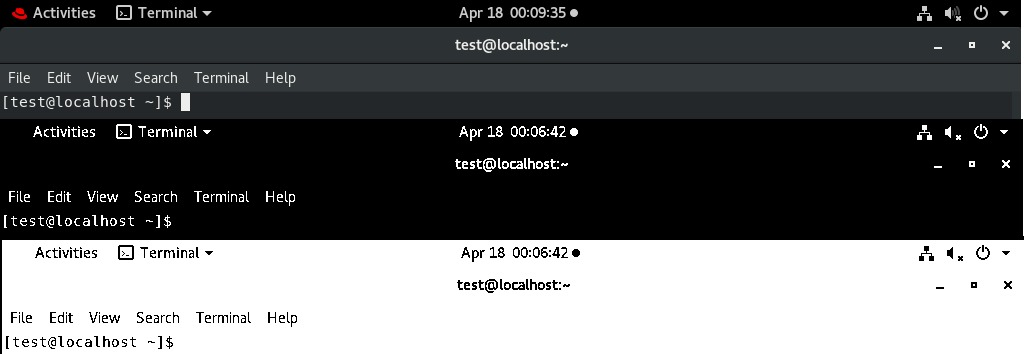
\includegraphics[width=1\textwidth,clip]{obrazky-figures/OCR_conversion.jpg}
	\caption{Steps of image preprocessing for Optical Character Recognition tool Tesseract, from the top: the original image, the binarized image, the inverted binarized image}
	\label{ocr_conversion}
\end{figure}

Listing \ref{OCR_text1} demonstrates the results obtained from the image, where the source image contains white text on a black background. The Tesseract's OCR engine manages to extract certain strings from the screen, although the results are not reliable and thus may lead to false-positive reports during the test execution.  

\begin{lstlisting}[caption={Text generated from the binarized image in Figure \ref{ocr_conversion}},label={OCR_text1}]
Pet) Terminal ~ EV ee muerre. Ty Pa) Ones
Peels ee?

Ca sa
[test@localhost ~]$ 
\end{lstlisting}

Listing \ref{OCR_text2} is showing the result of the character recognition when the image contains black text on a white background. When compared to Listings \ref{OCR_text1}, it proves an increase of the efficiency achieved with the implemented optimization. The result contains almost all strings shown on the screen with some random characters created as an attempt to read icons located in the right top corner of the window. The image conversions are achieved through methods from the \textit{OpenCV} library. 

\begin{lstlisting}[caption={Text generated from the inverted binarized image in Figure \ref{ocr_conversion}},label={OCR_text2}]
 Activities Terminal ~ Apr 18 00:22:36 AO Or
test@localhost:~ - 9 x

File Edit View Search Terminal Help
[test@localhost ~]$
\end{lstlisting}

Further experiments have shown additional issues with text formatting and recognition of certain letters. These facts lead to another set of optimizations that were implemented to avoid false positive test cases. A search for a string containing multiple words with white spaces might fail because the result might not contain all the white-spaces. Strings containing symbols …, -, \_, and — could be easily exchanged during the recognition. Those letters are not as important as letters representing the actual text. Therefore, a search for a match in the extracted text is performed twice. The first attempt tries to match the string with white spaces and full formatting. If that attempt fails, the second attempt breaks the string into words and tries to match every word separately. The second attempt is also followed by a warning message that the string was not matched in the original version.

The Tesseract has shown occasional difficulties with recognition of similarly looking letters. The most affected character was \textbf{I} exchanged for \textbf{1}, followed by \textbf{S} exchanged for \textbf{5}. Despite these occasional cases, the implementation works quite reliably both during the test generation process and the execution process. Nevertheless, the time consumed by taking screenshots during the generation process is significant. Therefore, the developed tool has the ability to disable the generation of the OCR steps during the generation of test cases through the command line parameter \texttt{-{}-disable-OCR}. If the generated test cases already contain steps performing OCR checks and are intended to be executed without them, the tests can be executed with the shell variable \texttt{OCR=False}. The defined variable will cause skipping of the OCR checks, although they will still be shown in the test logs as executed. This is caused by the limitation of the behave framework as it only allows to skip whole test scenarios. The test results executed with the variable will contain a warning message about skipped OCR steps.

\subsection{Implemented Steps}
The results obtained from experiments with the OCR were implemented to a single behave step. The step contains a string variable that should be found on the screen at specific moment during the test execution. The process involves taking a screenshot via \texttt{gnome-screenshot} utility. It continues with image preprocessing and extraction of the text from two variants of images. Finally, an assertion is made to confirm the presence of the string on the screen. Listing \ref{ocr_test} contains a test case generated for \textit{Gedit} flatpak, in this case the OCR should confirm the presence of the \textit{Save} button on the screen. The introduced optimizations from the last section should help to avoid false-positive results. However, if the OCR fails to find the string on the screen, the error message printed to a log will contain all the extracted text. This should help the testers with easier identification of false-positives.

\begin{lstlisting}[language=Gherkin,caption={Test case demonstrating the OCR integration in test cases},label={ocr_test}]
    @18_Save
    Scenario: org.gnome.gedit: 18_Save
      * Start: "org.gnome.gedit" via command in session
      * State: "push button" "Save" "showing" is "True"
      * OCR: "Save" is shown on the screen
      * Action: "click" "Save" "push button"
      * State: "file chooser" "Save As" is shown
\end{lstlisting}


% implementation and testing, running in a VM and stuff

% An example of the generated test case scenario is available ....

\chapter{Testing and Results}
The result of the generation process is available in a folder structure containing generated test cases, configuration files, and scripts for execution in the CI environment. Generated test cases are located in the file named \texttt{generated.feature}. The file contains all the test cases divided into so-called scenarios. Each scenario has a unique name starting with character \texttt{@} that allows single test execution if required. All tests are executable by issuing a command \texttt{behave} in the generated project folder. The tests are also respecting the cleanup commands which are set in \texttt{apps.yaml}. The cleanup is always executed after the finish of the test, regardless of the result of the executed tests. Execution of \texttt{behave} either prints steps from a test scenario to standard output or can generate an HTML log. This log format is more suitable for examination of the results executed in the CI environment accessible through the web interface. Thanks to the setup done by the \textit{qecore} library, the test reports have embedded logs, videos from the test runs, and a screenshot generated in a moment, when the test case fails. The next several sections describe the testing performed on several applications and the evaluation of the achieved results. The section starts with a short description of an application, followed by a result achieved by the proposed test generation tool.  

\section{Model/Event Coverage}
Test coverage can be measured in several ways. One option is to measure the amount on nodes and events covered by tests. The model is measured as the amount of the nodes involved in the test cases from the overall number of nodes in the model. It is expected that this coverage will always cover 100\% of the nodes. However, with applications that contain richer GUI, some of the nodes might be hidden or the generator will not be able to derive the sequence that will be able to access those nodes. This especially applies to cases when the generator will be used on a new application that contains some special layout or the action on the given node could not be executed for unknown reason. The generator skips the whole test case, generates an error message, and proceeds to the next test case. 

Nodes that are not covered by tests, along with test sequences that are involved, are printed in a report after the test generator finishes.  The nodes or test sequences reported as failed must be evaluated manually with several possible outcomes:
\begin{enumerate}
    \item a bug in the tested application
    \item a bug in the accessibility (e.g. incorrectly reported coordinates)
    \item an imperfection/bug in the test generator
    \item the tested application is affected by the previous test case (change in the settings/layout), an additional cleanup must be added to \texttt{apps.yaml}
\end{enumerate}
The report not only serves as a feedback from the generator about potential issues but it also measures the event coverage. The event coverage measures the amount of actions executed on the model and it is a common technique used in GUI testing\cite{NguyenBao2014Gait}.

\section{Code Coverage}
Another possibility is to use a tool \verb|gcov|, which is a standard part of the GNU development tools. The purpose of the tool is Code Coverage Analysis and it was designed to find dead or unexecuted code. Code coverage analysis can be characterized by the following steps: 
\begin{enumerate}
  \item Find the areas of a program not exercised by the test suite.
  \item Create additional test cases to exercise the dead code, thereby increasing code coverage.
  \item Determine a quantitative measure of code coverage, which is an indirect measure of quality.
\end{enumerate}

To obtain a measurement of the code coverage, it's required to compile the application with \verb|gcc|/\verb|g++| and two extra parameters \verb|-fprofile-arcs| and \verb|-ftestcoverage|. Running the compiled binary with a \verb|gcov| tool will yield a percentage of the executed code located in source file. Measurements can be obtained for any software written in C/C++.\cite{gcov} 

To obtain measurements, tests must be executed with the custom binary, compiled with mentioned parameters. Once the custom binary is executed, files with extensions \texttt{.gcda} and \texttt{.gcno} should appear in the directory where the binary is located. Measurements are aggregated throughout the test execution and the code coverage is reported to the special files with mentioned extensions. Then, the \texttt{lcov} tool is used to aggregate the measurements and generate a report in two steps (Code Listing \ref{lcov_report}). The first command takes the\texttt{.gcda} and \texttt{.gcno} files and generates \texttt{.info} file with coverage info. The second command takes the \texttt{info} file and generates a detailed HTML report. The report contains every source file (\texttt{.c} file) along with percentage of covered functions and lines.

\begin{lstlisting}[language=Gherkin,caption={Shell commands used to generate an HTML report with \texttt{lcov} tool},label={lcov_report}]
    lcov -c -d . -o app.info
    genhtml -o lcov_report -s --legend app.info --ignore-errors
\end{lstlisting}


According to the GTK website\footnote{\url{https://www.gtk.org/}}, the framework supports JavaScript, Python, Rust, Vala, C, and Perl. The \verb|gcov| method of measuring the test coverage is only possible for C and Vala.    
%test coverage, node coverage, action coverage
\newpage
\section{GNOME Terminal Tests}
% code coverage, explanation of achieved coverage
GNOME Terminal is one of the most important applications from the GNOME application stack. It is also known as \textit{Terminal} and it serves as a terminal emulator for accessing a UNIX shell environment. The application can be used to run programs available on the system\footnote{\url{https://help.gnome.org/users/gnome-terminal/stable/introduction.html.en}}. Compared to the majority of GNOME applications, \textit{Terminal} does not contain as many UI elements. Therefore, it was used for the initial development of the test generator. Shortly after the first proof of concept was tested, the list of applications was extended to \textit{LibreOffice Start Center} and \textit{Gedit}. 

\subsection{Setup and Cleanup}
Greater part of test cases is performing some changes of settings either via \textit{Preferences} dialog or through menus located at the top of the window. Preferences can change various aspects of the application, including encoding, layout of widgets, and color schemes. Those changes need to be set back to default values to make sure that test cases won't affect subsequent test cases. In \textit{Terminal}, this is achieved through 2 cleanup commands executed between applied test sequences (Code Listing \ref{gnome-terminal-cleanup}). Testing was performed on rpm package gnome-terminal-3.28.3-1.el8.x86\_64, Red Hat Enterprise Linux 8.3.

\begin{lstlisting}[caption={Final test generator report},label={gnome-terminal-cleanup}]
    dconf reset /org/gtk/Settings/Debug/enable-inspector-keybinding
    dconf reset -f /org/gnome/terminal/legacy/
\end{lstlisting}

\subsection{Test Generation and Results}

Listing \ref{gnome-terminal-report} contains the final report and summarizes the testing performed on \textit{Terminal}. The developed test generator was able to generate 485 test cases while covering the 1701 events in the application. Tests are covering menus, several smaller dialogs, and a \textit{Preferences} window.

\begin{lstlisting}[caption={Final test generator report},label={gnome-terminal-report}]
    Event Coverage Report:
        Covered Events: 1700/1702
    Number of covered Nodes: 516
    Number of Generated Test Cases: 485 
    Nodes without the coverage:
    Edit:menu:click => Preferences:menu item:click => :list item: 
            => Menu:toggle button:click
    Help:menu:click => About:menu item:click => :link:Click
    No errors found!
    Generation time: 1:53:52.676497
\end{lstlisting}

\textit{Terminal} also offered a good demonstration of how nodes are expanded during the test generation. Initially, the generator scans the tree for the available nodes and builds a model from 104 available nodes (widgets) and derives 96 test sequences (Figure \ref{gnome-terminal-graph1}). The Generator proceeds with the application of sequences and continuously expands the model to the final amount of 516 nodes and 485 derived test cases (Figure \ref{gnome-terminal-graph2}).

\begin{figure}[H]
	\centering
	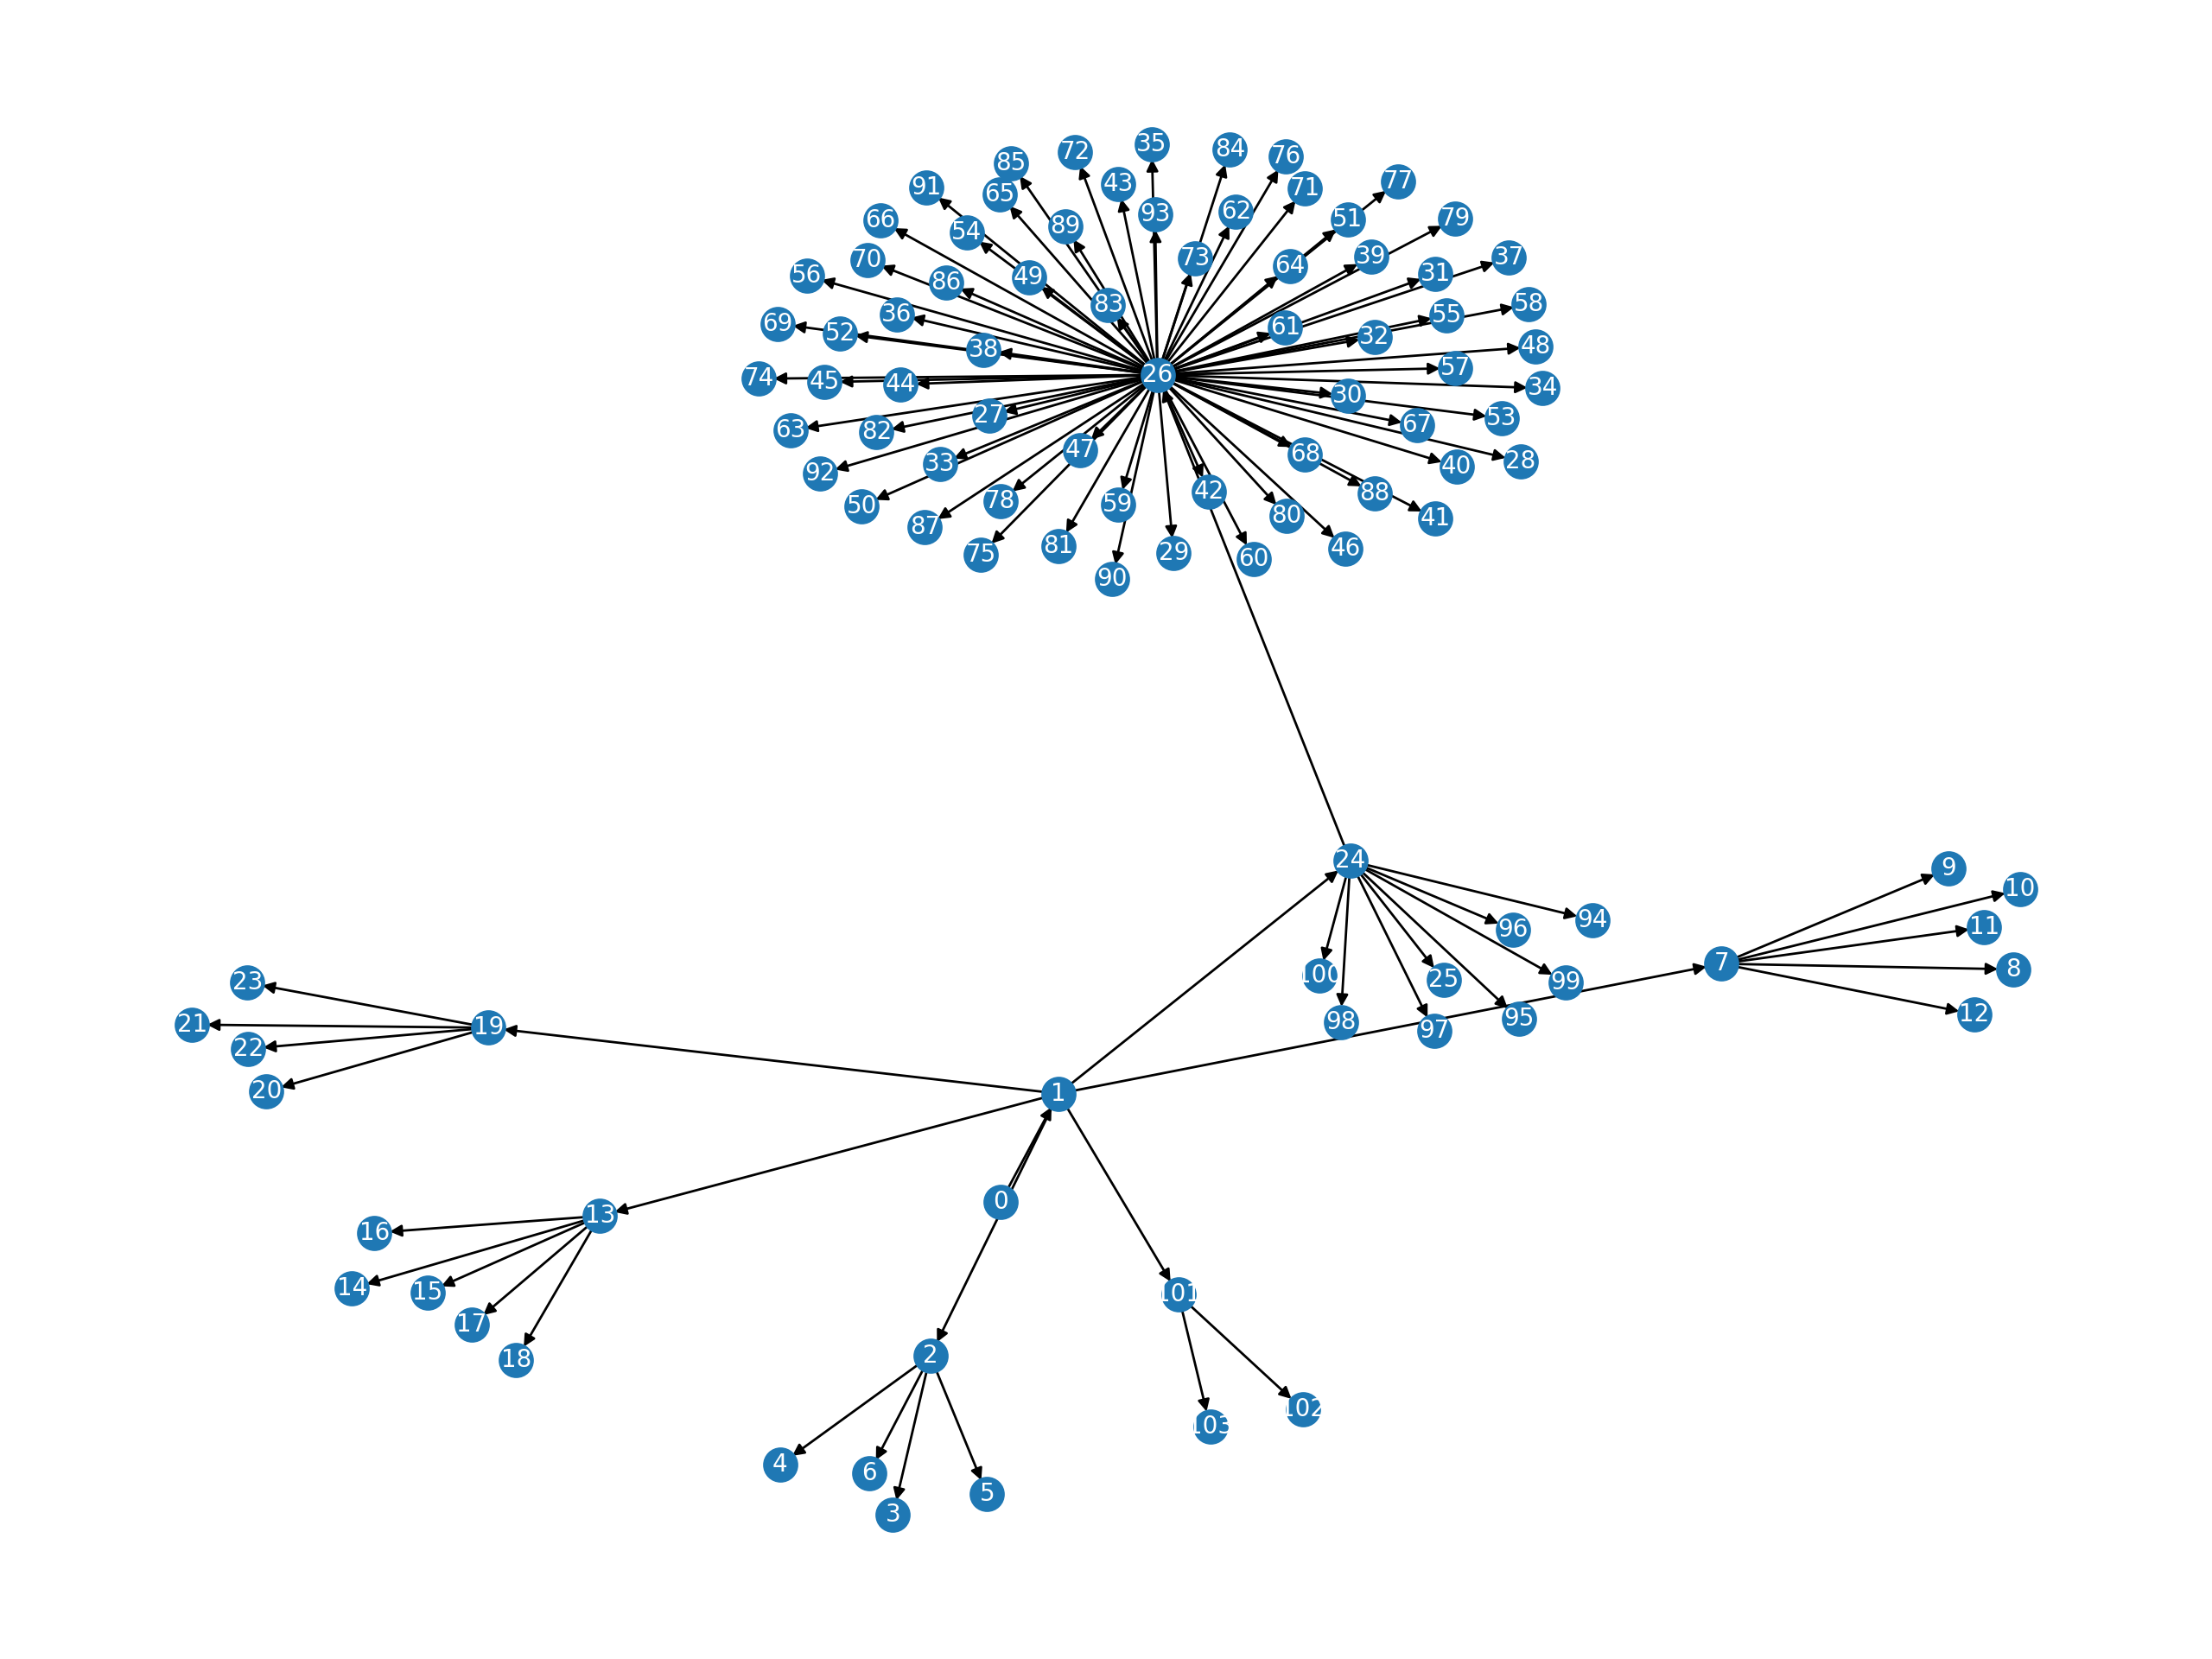
\includegraphics[width=0.85\textwidth,clip]{obrazky-figures/gnome-terminal_n_start.png}
	\caption{Initial event flow graph of the test sequence available after the start of \textit{Terminal}}
	\label{gnome-terminal-graph1}
\end{figure}

\begin{figure}[H]
	\centering
	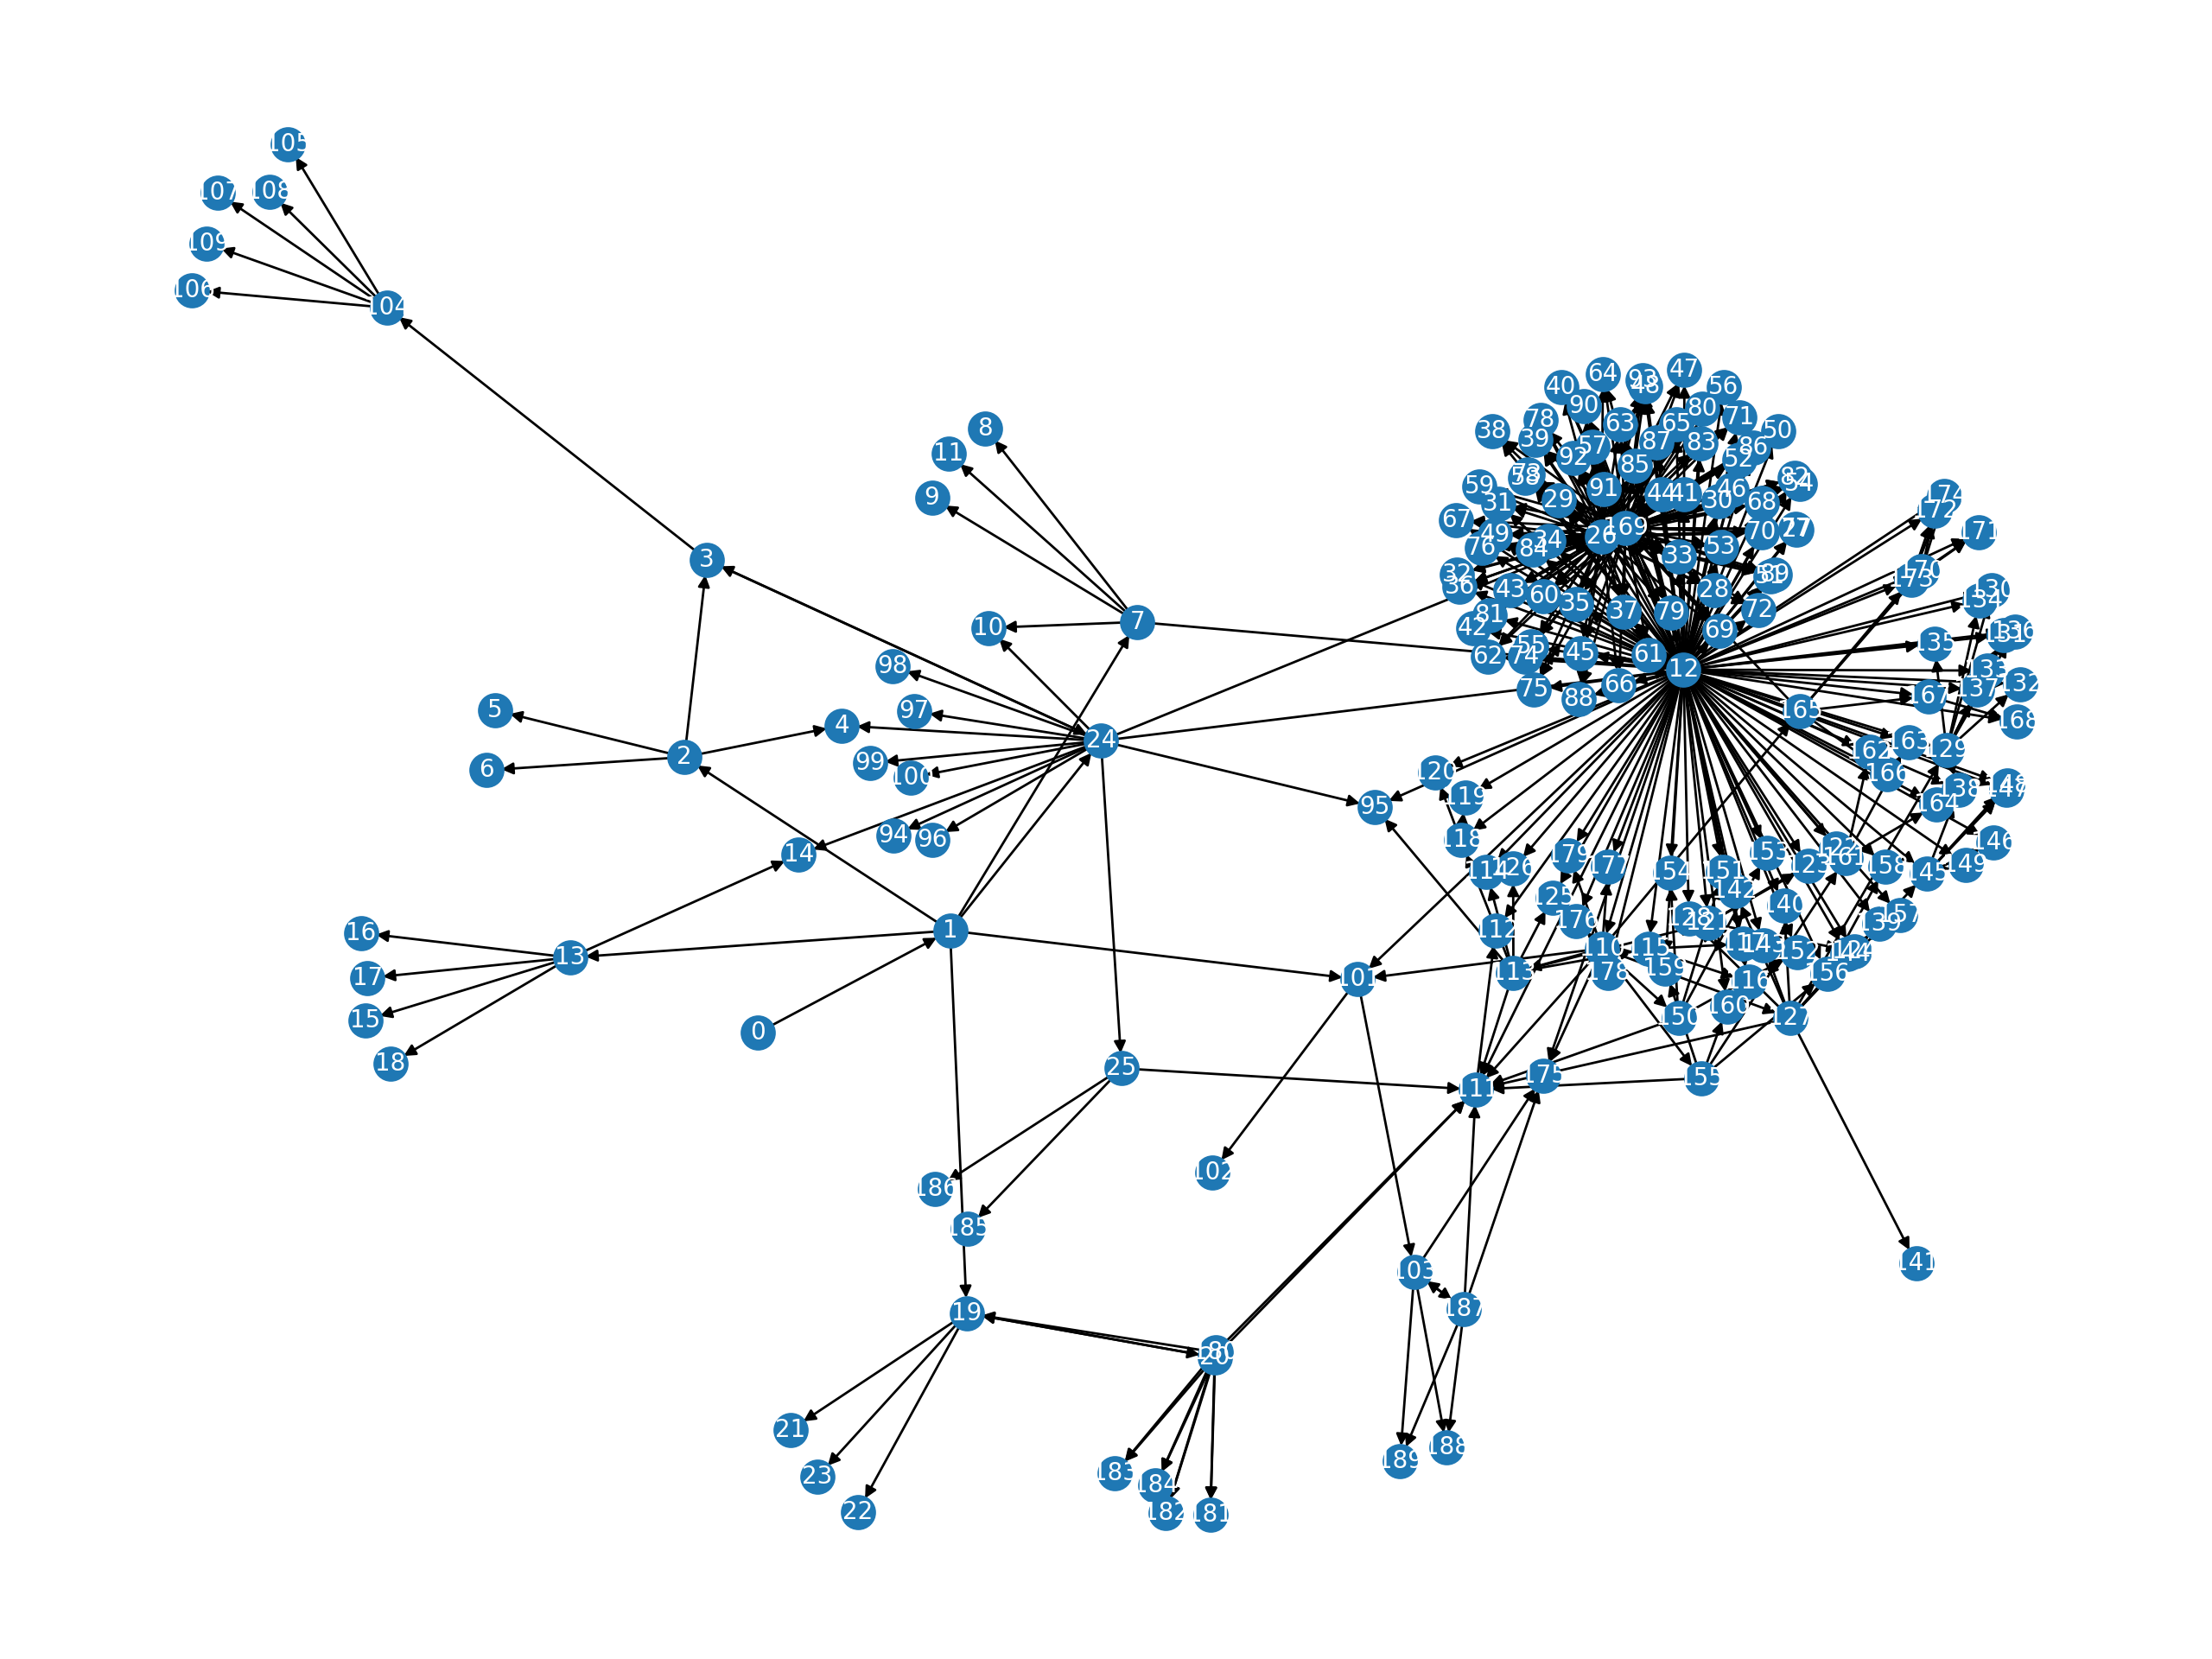
\includegraphics[width=0.85\textwidth,clip]{obrazky-figures/gnome-terminal_n_final.png}
	\caption{Expanded event flow graph of test sequences, the graph demonstrates node expansion during the test generation}
	\label{gnome-terminal-graph2}
\end{figure}

\begin{figure}[H]
	\centering
	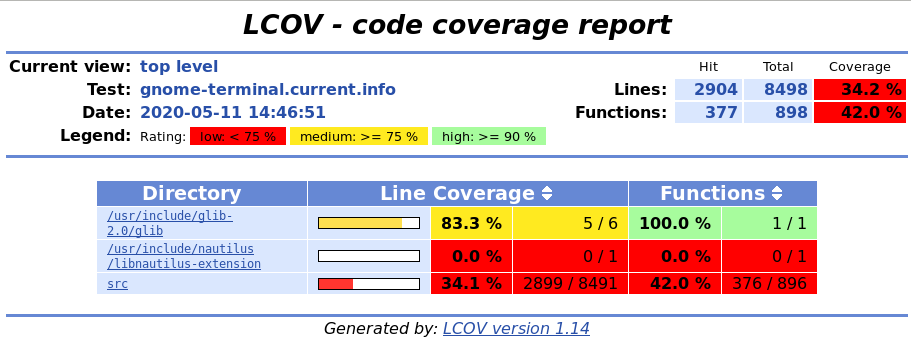
\includegraphics[width=0.8\textwidth,clip]{obrazky-figures/gnome-termina-coverage.png}
	\caption{LCOV code coverage report documents the achieved code coverage with generated test cases}
	\label{gnome-terminal-coverage}
\end{figure}

Generated test cases covered 34.2\% lines of source code and executed 42\% of functions (Figure \ref{gnome-terminal-coverage}). As described in the report, the coverage resides in the low category. After looking to the report in detail and reading the comments in source code, the analysis has shown that several parts of the GUI are not executed by the tests. It has revealed functions that are handling shortcuts that are not covered in the test cases. It is also expected that a large portion of code is related to non-GUI operations which are not covered in tests at all.

\section{Gedit (flatpak)}
\section{LibreOffice StartCenter}
%window detection, spawning application withing - changing window
%bug found
\section{Comparison with Existing Test Suites}
As discussed in Chapter \ref{proposed_solution}, the approach to application testing done by this work combines several testing techniques and takes advantage of existing testing frameworks and libraries. To the best of my knowledge, there is no tool currently available that tries to achieve the same goal, targeted on applications built for the GNOME environment. The closest related solutions were described in Section \ref{TEMA_TOOLSET}. However, the solution is designed for applications with different development cycle, where a model is being developed before a prototype of the application is available. The proposed solution derives the model of the SUT from the metadata provided by the accessibility.

When it comes to solutions used for the test automation for GNOME applications, several record and replay tools were described in Section \ref{record_replay}. The proposed solution utilizes \textit{dogtail} combined with framework \textit{behave}, so the generated test cases are executable even after the generation process is finished.

Scripted test cases are written by humans (testers). Their goal is either to automate scenarios that cover key features in applications or to create scenarios based on previously discovered bugs and defects. However, the proposed test generator is a semi-smart tool. Errors and crashes that occur during the generation process are recognized and reported with a reproducer. The potential problem is with the semantics of the test cases. The test generator can apply a sequence of actions to the application although it cannot decide whether the outcome is expected. Therefore, the proposed tool should aid the testers with the development of the test automation right after the executable version of an application is available. The main advantage is in the exploratory testing performed during the test generation. The test generator can sequentially execute available events (test sequences) and possibly help testers to avoid drawbacks of manual testing. The report from the test generation process will also point out the widgets that were not covered by the exploratory testing and therefore they are not covered by the test cases. An additional benefit is provided by the fairly quick availability of the working test automation. Testers can push either all or a subset of test cases in the CI environment. Any test case can be reviewed and updated, new test cases could be written with available \textit{behave} steps or a new step definition can be added. Generated test cases can be merged with the test automation available from the previous versions, if it is not too obsolete.

The test generator itself is a piece of software as well. It is designed to work with as many applications as possible, therefore, the implementation is as general as possible. If a tested application reveals flaws that may be fixed within the test generator. The fixes must maintain the approach that the implementation has to be as general as possible, thus they will not affect the other components. Therefore, if the fix is too application-specific, the effort that needs to be done to include the fix in the test generator should not be greater than developing a custom test case.

In conclusion, generated test cases are not comparable with the currently available test automation developed with script-based tools. The goal of generated test cases is to cover as many events in applications as possible whereas the currently available test suites are focused on automation of the most essential task performed by users and tasks in which bugs and defects occurred in the past. This comparison does not include unit tests or any other white-box tests performed on the library level.


\chapter{Conclusion}

  \else
    \input{projekt-01-kapitoly-chapters}
  \fi
  
  % Kompilace po částech (viz výše, nutno odkomentovat)
  % Compilation piecewise (see above, it is necessary to uncomment it)
  %\subfile{projekt-01-uvod-introduction}
  % ...
  %\subfile{chapters/projekt-05-conclusion}


  % Pouzita literatura / Bibliography
  % ----------------------------------------------
\ifslovak
  \makeatletter
  \def\@openbib@code{\addcontentsline{toc}{chapter}{Literatúra}}
  \makeatother
  \bibliographystyle{bib-styles/Pysny/skplain}
\else
  \ifczech
    \makeatletter
    \def\@openbib@code{\addcontentsline{toc}{chapter}{Literatura}}
    \makeatother
    \bibliographystyle{bib-styles/Pysny/czplain}
  \else 
    \makeatletter
    \def\@openbib@code{\addcontentsline{toc}{chapter}{Bibliography}}
    \makeatother
    \bibliographystyle{bib-styles/Pysny/enplain}
  %  \bibliographystyle{alpha}
  \fi
\fi
  \begin{flushleft}
  \bibliography{projekt-20-literatura-bibliography}
  \end{flushleft}

  % vynechani stranky v oboustrannem rezimu
  % Skip the page in the two-sided mode
  \iftwoside
    \cleardoublepage
  \fi

  % Prilohy / Appendices
  % ---------------------------------------------
  \appendix
\ifczech
  \renewcommand{\appendixpagename}{Přílohy}
  \renewcommand{\appendixtocname}{Přílohy}
  \renewcommand{\appendixname}{Příloha}
\fi
\ifslovak
  \renewcommand{\appendixpagename}{Prílohy}
  \renewcommand{\appendixtocname}{Prílohy}
  \renewcommand{\appendixname}{Príloha}
\fi
%  \appendixpage

% vynechani stranky v oboustrannem rezimu
% Skip the page in the two-sided mode
%\iftwoside
%  \cleardoublepage
%\fi
  
\ifslovak
%  \section*{Zoznam príloh}
%  \addcontentsline{toc}{section}{Zoznam príloh}
\else
  \ifczech
%    \section*{Seznam příloh}
%    \addcontentsline{toc}{section}{Seznam příloh}
  \else
    % \section*{List of Appendices}
    % \addcontentsline{toc}{section}{List of Appendices}
  \fi
\fi
  \startcontents[chapters]
  \setlength{\parskip}{0pt} 
  % seznam příloh / list of appendices
  % \printcontents[chapters]{l}{0}{\setcounter{tocdepth}{2}}
  
  \ifODSAZ
    \setlength{\parskip}{0.5\bigskipamount}
  \else
    \setlength{\parskip}{0pt}
  \fi
  
  % vynechani stranky v oboustrannem rezimu
  \iftwoside
    \cleardoublepage
  \fi
  
  % Přílohy / Appendices
  \ifenglish
    
\chapter{Abbreviations}
\renewcommand{\arraystretch}{1.2}
\begin{tabular}{lp{12cm}}%
\textbf{ATK} & Accessibility Toolkit \\
\textbf{AT-SPI} & Assistive Technology Service Provider Interface \\
\textbf{CI} & Continuous Integration \\
\textbf{CD} & Continuous Delivery \\
\textbf{GAIL} & GNOME Accessibility Implementation Library \\
\textbf{GNU} & GNU's Not Unix \\
\textbf{GNOME} & GNU Network Object Model Environment \\
\textbf{GTK} & The GNOME Toolkit \\
\textbf{LTSM} & Long Short Term Memory \\
\textbf{RRN} & RecurrentNeural Network \\
\textbf{OCR} & Optical Image Recognition \\
\textbf{OpenCV} & Open Source Computer Vision Library \\
\end{tabular}


\chapter{Setup Instructions}


\chapter{Examples of Generated Test Scenarios}

% % This file should be replaced with your file with an appendices (headings below are examples only)

% % Placing of table of contents of the memory media here should be consulted with a supervisor
% %\chapter{Contents of the included storage media}

% %\chapter{Manual}

% %\chapter{Configuration file}

% %\chapter{Scheme of RelaxNG configuration file}

% %\chapter{Poster}

% \chapter{How to use this template}
% \label{jak}

% This chapter describes individual parts of the template, followed by a brief instructions on how to use it. If you have any questions, comments etc, feel free to email them to \texttt{sablona@fit.vutbr.cz}.

% \section*{Template parts description}

% Once you extract the template, you will find the following files and directories:
% \begin{DESCRIPTION}
%   \item [bib-styles] Literature styles (see below). 
%   \item [obrazky-figures] Directory for your images. Currently contains \texttt{placeholder.pdf} (a.k.a TODO image -- see below) and image keep-calm.png to demonstrate inserting raster images (you don't submit these images with your thesis). It is advised to use shorter directory name, so that it is only in your chosen language.
%   \item [template-fig] Template images (BUT logo).
%   \item [fitthesis.cls] Template (design definition).
%   \item [Makefile] Makefile used to compile the project, count standard pages etc. (see below).
%   \item [projekt-01-kapitoly-chapters-en.tex] File for Your text (replace it's contents).
%   \item [projekt-20-literatura-bibliography.bib] Reference list (see below).
%   \item [projekt-30-prilohy-appendices-en.tex] File for your appendices (replace it's contents).
%   \item [projekt.tex] Main project file -- definitions of formal parts.
% \end{DESCRIPTION}

% The style of literature in the template is from Ing. Radek Pyšný \cite{Pysny}, whose work was improved by prof. Adam Herout, dr. Jaroslav Dytrych and Mr. Karel Hanák to comply with the norm and support all frequently used types of citations. Its documentation can be found in the appendix

% Aside from compilation to PDF, the Makefile also offers additional functions:
% \begin{itemize}
%   \item rename files (see below),
%   \item count standard pages,
%   \item run a wave that adds unbreakable spaces,
%   \item compress (zip) the result, ready to be sent to your supervisor and checked (make sure that all the files you've added are included, if not, add them manually).
% \end{itemize}

% Keep in mind that the wave is not perfect. You always need to check whether or not there is something inappropriate at the end of a line manually -- see Online language handbook\footnote{Internetová jazyková příručka \url{http://prirucka.ujc.cas.cz/?id=880}}.

% Similar rules apply also in English - see eg. article Run Ragged\footnote{Run Ragged\url{https://24ways.org/2013/run-ragged/}}, according to which there should be no prepositions, dash or short words (2--3 letters) at the end of the lines, the two lines following each other should not end with a comma and line break should not be also in the phrases from 2-3 words.

% \paragraph {Pay attention to page numbering!} If the table of contents is 2 pages long and the second page contains only \uv{Enclosures} and \uv{List of enclosures} (but there is no enclosure), the page numbering is changed by 1 (table of contents and contents \uv{mismatch}). The same thing happens if the second or third page contains only \uv{References} and there's a chance that this can occur in other situations too. There are multiple solutions to this (from editing the table of contents, setting the page counter all the way to more sophisticated methods). \textbf{Check the page numbering before you submit your thesis!}

% \section*{Recommendations for working with the template}

% \begin{enumerate}
%   \item \textbf{Make sure you have the latest version of template.} If you have a template from last year, there should be a newer version (updated information, fixed errors etc.) available at the faculty or study advisor web pages.  
%   \item \textbf{Choose a language}, that you want to use for your technical report (czech, slovak or english) and consult your supervisor about your choice (unless it was agreed upon in advance). If your language of choice is not czech, set the respective template parameter in file projekt.tex (e.g.: \verb|document|\verb|class[english]{fitthesis}| and translate the declaration and acknowledgement to english or slovak).
%   \item \textbf{Rename the files.} When you extract the files, there should be a file named projekt.tex. If you compile it, it will create a PDF with technical report named projekt.pdf. If multiple students send their supervisor projekt.pdf to have it checked, they have to rename them. For that reason, it is advised to rename the file so that it contains your login and (if needed, abbreviated) work topic. Avoid using spaces, diacritic and special symbols. An appropriate name for your file can look like this: \uv{xlogin00-Cleaning-and-extraction-of-text.tex}. You can use the included Makefile to rename it: 
% \begin{verbatim}
% make rename NAME=xlogin00-Cleaning-and-extraction-of-text
% \end{verbatim}
%   \item Fill in the required information in file, that was originally named projekt.text, that means type, year (of submission), thesis title, author's name, department (according to specification), supervisor's titles and name, abstract, keywords and other formal requirements.
%   \item Replace the contents of thesis chapters, references and enclosures files with the contents of your technical report. Individual enclosures or thesis chapters can be saved to separate files -- if you choose this approach, it is advised to comply with the file naming convention, and the number will be followed by the chapter title.
%   \item If you don't need enclosures, comment the respective part in projekt.tex and erase everything from the corresponding file or delete it. Don't try to come up with an aimless enclosures just to have something in that file. An appropriate enclosure can be the contents of included memory medium.
%   \item Delete the chapter and attachment files for a language you haven't used (with or without \texttt{-en}).
%   \item Assignment that you download in PDF from FIT IS (link \uv{Thesis assignment}) save to file \texttt{zadani.pdf} and enable its insertion into work by appropriate template parameter (\verb|document|\verb|class[zadani]{fitthesis}|) in \texttt{projekt.tex}.
%   \item If you don't want to print references in color (i cannot recommend this without consulting your supervisor), you'll need to create a second PDF for printing and set the template printing parameter:\\ (\verb|document|\verb|class[english,zadani,print]{fitthesis}|). Colored logo must not be printed in black and white.
%   \item The binder templace where the thesis will be typeset can be generated in faculty IS at specification. Can be enabled for dissertation using the \tt cover \rm parameter in template.
%   \item Don't forget that source files and (both versions) PDF has to be on a CD or other medium included in the technical report.
% \end{enumerate}

% \subsection*{Instructions for double-sided printing}
% \begin{itemize}
% \item \textbf{It is advised to consult your supervisor about double-sided printing.}
% \item If you used double-sided printing for your thesis and it's thickness is smaller than the thickness of the binder, it doesn't look too good.
% \item Enabled using the following template parameter:\\ \verb|\document|\verb|class[twoside]{fitthesis}|
% \item After printing a double-sided sheet, make sure that the canon of page construction is in the same position on both pages. Inferior printers with duplex printing unit usually cause a shift by 1--3 mm. This can be solved with some printers. Print the odd pages first, put them back into the same tray and print the even pages.
% \item Leave a blank page after title page, table of contents, references, list of tables, list of appendices and other lists to make sure that the following part starts on an odd page (\texttt{\textbackslash cleardoublepage}).
% \item Check the final result thoroughly.
% \end{itemize}

% \subsection*{Paragraph style}

% Paragraphs have justified alignment and there are multiple methods for formatting them. In Czech paper literature, a paragraph indentation method is common, where each paragraph of the text have the first line of a paragraph indented by about one to two quads, that is, about two widths of the capital letter M of the base text (always about the same preselected value). In this case, the last line of the previous paragraph and the first line of the following paragraph are not separated by a vertical space. The interleaving between these lines is the same as the interleaving inside the paragraph \cite{fitWeb}.

% Another method is indenting paragraphs, which is common for electronic typesetting and for English texts. In this method, the first line of a paragraph is not indented and a vertical space of approximately half of a line is inserted between the paragraphs. Both methods can be used in the thesis, however, the latter method is often more suitable. Methods should not be combined.

% One of the above methods is set as the default in the template, the other can be selected by the template parameter \uv{\tt odsaz\rm }.


% \subsection*{Useful tools} 
% \label{nastroje}

% The following list is not a list of all useful tools. If you have experience with a certain tool, feel free to use it. However, if you don't know which tool to choose, consider the ones listed below:

% \begin{description}
% 	\item[\href{http://miktex.org/download}{MikTeX}] \LaTeX{} for Windows -- a distribution with simple installation and great automated package downloading. MikTeX even has it's own editor, but I highly recommend TeXstudio.
% 	\item[\href{http://texstudio.sourceforge.net/}{TeXstudio}] Portable opensource GUI for \LaTeX{}. Ctrl+click switches between source text and PDF. Integrated spell checker\footnote{Spell checker for czech version can be installed from \url{https://extensions.openoffice.org/de/project/czech-dictionary-pack-ceske-slovniky-cs-cz}}, syntax highlighter etc. To use this tool, you need to first install MikTeX or another \LaTeX{} distribution.
%     \item[\href{http://www.winedt.com/}{WinEdt}] A good combination for Windows is WinEdt + MiKTeX. WinEdt is a GUI for Windows, and if you want to use it, you need to first install \href{http://miktex.org/download}{MikTeX} or \href{http://www.tug.org/texlive/}{TeX Live}.
%     \item[\href{http://kile.sourceforge.net/}{Kile}] Editor for KDE (Linux) desktop environment. Real-time preview. To use this tool, you need to have \href{http://www.tug.org/texlive/}{TeX Live} and Okular installed.
% 	\item[\href{http://jabref.sourceforge.net/download.php}{JabRef}] Neat and simple Java program for bibliography (references) file management. No need to learn anything -- provides a simple window and a form for entry editing.
% 	\item[\href{https://inkscape.org/en/download/}{InkScape}] Portable opensource vector graphic (SVG and PDF) editor. Excellent tool to use to create images for technical text. Difficult to master, but the results are worth it.
% 	\item[\href{https://git-scm.com/}{GIT}] Great tool for teamwork when it comes to projects, but can be incredibly useful even to a single author. Simple version control system, backup options and transfer between multiple computers.
% 	\item[\href{http://www.overleaf.com/}{Overleaf}] Online \LaTeX{} tool. A real-time compilation of source text that allows for simple collaboration (supervisor can continuously keep an eye on the progress made), move to a place in source file just by clicking in the PDF preview, spell checker etc. There are some limitations to what you can do if you want to use it for free (some people are comfortable with it for dissertation, others can run into it while they write a~bachelor's thesis) and it is rather slow for long texts. FIT BUT has for students and employees of a license, which can be activated on \url{https://www.overleaf.com/edu/but}.
% \end{description}

% Note: Overleaf does not use template Makefile -- to get compilation to work, you need to go to the menu and select \tt projekt.tex \rm as s Main document.

% \chapter{Writing english texts}
% \label{anglicky}
% This chapter is taken from web pages of Jan Černocký \cite{CernockyEnglish}.

% A lot of people write their technical reports in english (which is good!), but they make a~lot of unnecesary mistakes (which is bad!). I'm not an english export myself, but I've been using this language for a while now to write, read and even communicate -- this chapter contains a handful of important things. If you want to be certain that your thesis or article is 100\,\% correct, your best bet is to hire a native speaker (preferably someone who is technically capable and understands what you write about \ldots).


% \section*{In general}

% \begin{itemize}
%   \item{Before you jump into it head first, I suggest you read a handful of technical articles written in english and try to remember or preferably understand how you should approach writing one yourself.}
%   \item{Always use a spell checking tools -- built in tools in Word, or in OpenOffice. If you work on Linux, I suggest you use ISPELL. Some spell checking (I think it's the one in PSPad) are not very good and ignore a lot of mistakes.}
%   \item{Use grammer checking tools. I'm not entirely sure if there is one available for Linux, but the one in Word is fairly decent and if it underlines anything with green color, it's probably wrong. You can even copy and paste Latex source code here, fix any and all grammar errors and save it as a clean text again. If you use vim, there's a~built in grammar checking tool too, and it's capable of detecting typos and errors in basic grammar. Write this in the first line of your thesis tex file:
%   \begin{verbatim}
%     % vim:spelllang=en_us:spell
%   \end{verbatim}
%   (alternatively \texttt{en\_gb} for OED english) \textit{Editor's note:} There is a very good online tool Grammarly\footnote{\url{https://www.grammarly.com/}}, with free basic version.
%   }
%   \item{Online dictionaries are good, but don't rely on them in every situation. Usually you get multiple choices and not all of them are correct for the given context.}
%   \item{\begin{samepage}You can probably figure out what the correct option is by looking each option up and seeing the context in which they're used, example given: ``advantage/privilege/facility of approach''. Online dictionaries give you a handful of results. Look them up one by one using google search:
%   \begin{verbatim}
%     "advantage of this approach" 1100000 hits
%     "privilege of this approach" 6 hits
%     "facility of this approach"  16 hits
%   \end{verbatim}
%   I'm not saying it's 100\,\% correct, but at least you have something to go on. This can be used to find the correct connectives (e.g. ``among two cases'' or ``between two cases''?)\end{samepage}}
% \end{itemize}
       
% \section*{SVOMPT and concord}

% The structure of an english sentence is SVOPMT: SUBJECT VERB OBJECT MANNER PLACE TIME and there's no other way around it. It is not a flexible structure. There are possibly exceptions in things like a theater play, where something needs to be emphasized. Subject must be present in every single single sentence, people tend to forget as some languages have a sentence structure where the subject can be implicit and not mentioned. SVOMPT applies to dependent clauses too!
% \begin{verbatim}
%   BAD: We have shown that is faster than the other function. 
%   GOOD: We have shown that it is faster than the other function. 
% \end{verbatim}

% \noindent Concord or grammatical agreement between two words in a sentence -- it sounds silly, but people make countless mistakes here.

% \begin{verbatim}
%   he has 
%   the users have 
%   people were 
% \end{verbatim}

% \section*{Articles}

% Articles in english are a nightmare and almost all of us fail to use them correctly. The basic rule is, that if there's a particular noun, it's preceeded by ``the''. Definite articles must be in following phrases:
% \begin{verbatim}
%   the first, the second, ...
%   the last
%   the most (superlatives and adverbs) ...
%   the whole 
%   the following 
%   the figure, the table. 
%   the left, the right - on the left pannel, from the left to the right ... 
% \end{verbatim}

% \noindent On the contrary, there can't be an article when you're referring to a specific figure, chapter, etc.
% \begin{verbatim}
%   in Figure 3.2
%   in Chapter 7
%   in Table 6.4
% \end{verbatim}

% \begin{samepage}
% \noindent The use of ``a'' and ``an'' is based on the pronounciation, rather than how the word is written:
% \begin{verbatim}
%   an HMM
%   an XML
%   a universal model
%   a user
% \end{verbatim}
% \end{samepage}

% \section*{Verbs}

% Passive voice can be tricky -- regular verbs are usually not a problem, irregular verbs however are a common source of errors, typically
% \begin{verbatim}
%   packet was sent (rather than send)
%   approach was chosen (rather than choosed)
% \end{verbatim}
% \noindent \ldots most of the time, the spell checker will correct it, but it's not guaranteed.

% Tenses are a mess at times. If something just is in general, use present tense. If you did something, use past tense. If you got results that already exist and you just discuss them, use present tense. Try to avoid complicated tenses such as present perfect or worse past perfect if you're not 100\,\% sure.
% \begin{verbatim}
%   JFA is a technique that works for everyone in speaker recognition. 
%   We implemented it according to Kenny's recipe in \cite{Kenny}. 
%   12000 segments from NIST SRE 2006 were processed. When compared 
%   with a GMM baseline, the results are completely bad. 
% \end{verbatim}

% \section*{Sentence length and structure}

% \begin{itemize}
%   \item{Try to write shorter sentences. If you sentence is 5 lines long, it's probably a pain to read, if it can even be done.}
%   \item{Comma is a powerful tool and you should use it for your sentence structure. Use a~comma to seperate the initial dependent clause from the main independent clause. Sometimes it is appropriate to put a comma just before ``and'' (unlike other languages)!}
% \end{itemize}
% \begin{verbatim}
%   In this chapter, we will investigate into ... 
%   The first technique did not work, the second did not work as well, 
%   and the third one also did not work. 
% \end{verbatim}

% \section*{The specifics of a technical text}

% When writing a technical text, don't use common phrases such as
% \begin{verbatim}
%   he's
%   gonna
%   Petr's working on ...
% \end{verbatim}
% \noindent and others. The only tolerated thing is ``doesn't'', but you can never go wrong with ``does not''.

% \begin{samepage}
% \noindent Technical texts utilize passive voice a lot more than active voice: 
% \begin{verbatim}
%   BAD: In this chapter, I describe used programming languages. 
%   GOOD: In this chapter, used programming languages are described.
% \end{verbatim}
% \end{samepage}

% If you want to use active voice, it's more common to use ``we'', even though you work alone. ``I'', ``my'', etc. are only used when you need to emphasize that you are the person of utmost importance, for example in the conclusion or when discussing ``original claims'' in disertation.


% \paragraph{Common erros in words}

% \begin{itemize}
%   \item{Pay attention to his/hers, it's not ``it's'' but ``its''}
%   \item{Image is not picture, it's figure.}
%   \item{The connective is ``than'', not ``then'' -- bigger than this, smaller than this \ldots very common error! ``Then'' is used in the context of time.}
% \end{itemize}


% \chapter{Checklist}
% \label{checklist}
% This checklist was taken from a template for academic work, that is available on Adam Herout's blog \cite{Herout}, based on the ideas of Igor Szöke\footnote{\url{http://blog.igor.szoke.cz/2017/04/predstartovni-priprava-letu-neni.html}}, with their permission.

% A big part of the safety of air transport are checklists. They have checklists for basically anything and everything, even the most cut-and-dry procedures. If a pilot can get over the tedious process of marking off every single checkbox of a procedure, you can as well. Make a checklist of your own before you submit your thesis. \bf Yes, really: \rm print it, grab a pencil and check every single item on the list. It will make your life easier –- avoid unnecessary errors that can be fixed within a couple minutes –- as well as others', at very least your supervisor and reviewer of your thesis.

% \subsection*{Structure}
% \begin{checklist}
% 	\item You can tell that the assignment was completed just by looking at the chapter titles as well as their structures.
%     \item There is no chapter with less than four pages (except for introduction and conclusion). And if so, I discussed this with my supervisor and they gave me a green light.
% \end{checklist}

% \subsection*{Figures and charts}
% \begin{checklist}
% 	\item Every single image and table was checked and their position is close to the text that references them. In other words, they’re easy to find.
%     \item Every single image and table has a good enough caption, to ensure that the figure makes sense on it’s own, without the necessity to read the text. (There’s no harm in a long caption.)
%     \item If an image is taken from somewhere, it is mentioned in the caption: “Taken from [X].”
%     \item Texts in all images have a font size similar to the surrounding text (neither signifficantly larger, nor signifficantly smaller).
%     \item Charts and schemes are vector graphics (eg. in PDF).
%     \item Screenshots don‘t use lossy compression (they‘re in PNG).
%     \item All images are referenced in the text.
%     \item Axes in charts have their captions (name of the axis, units of measurement, values) and a grind if need be.
% \end{checklist}

% \subsection*{Equations}
% \begin{checklist}
% 	\item Identifiers and their indexes in equations are single letters (except for rather uncommon cases like $t_{max}$).
%     \item Equations are numbered.
%     \item All the variables and functions that haven‘t been explained yet are explained below (or rarely above) the equation.
% \end{checklist}

% \subsection*{Citations}
% \begin{checklist}
% 	\item \bf All used sources are cited. \rm
% 	\item URL adresses referencing services, projects, sources, github, etc. are referenced using \verb|\footnote{\url{…}}|.
%     \item URL adresses in citations are only present, if necessary – article is cited like an article (author, title, where and when was it published), not using URL.
%     \item Citations have author, title, publisher (conference title), year of publishing. If a~citation does not have either of these, there is a good explanation for this special case and my supervisor agreed.
%     \item If there is anything taken over from some other work in the program source code, it is properly cited therein in conformance with the license.
% 	\item If an essential part of the source code of the program is taken over, this is mentioned in the text of the thesis and the source is cited.
% \end{checklist}

% \subsection*{Typography}
% \begin{checklist}
% 	\item No line extends past the right margin.
%     \item There is no single-letter preposition at the end of a line (fixed using unbreakable space \verb|~|).
%     \item Number of image, table, equation, citation is never a first item of a new line (fixed using unbreakable space \verb|~|).
%     \item There is no space before a numeric reference to a footnote (like this\footnote{footnote example}, not like this \footnote{another footnote example}).
% \end{checklist}

% \subsection*{Language}
% \begin{checklist}
% 	\item I used spellchecker and there were no typos in the text.
%     \item I had someone else read my thesis (at least one person), that knows czech / slovak / english well.
%     \item Someone who knows english well checked the abstract  in a czech or slovak written abstract thesis.
%     \item No part of the text is written in second person (you).
%     \item If first person is used (i, we), a subjective matter is being described (i decided, i~designed, i focused on, i found out, etc.).
%     \item There are no colloquialisms in the text.
%     \item There are no {\it default} words in the text.
% \end{checklist}

% \subsection*{Result is on a data medium, i.e. software}
% \begin{checklist}
% 	\item I have a non-rewritable data medium ready.
%     \begin{itemize}
%     	\item CD-R,
%         \item DVD-R,
%         \item DVD+R in ISO9660 format (with RockRidge and/or Jolliet extension) or UDF,
%         \item SD (Secure Digital) card in FAT32 or exFAT format, the card is set to write-protected mode
%     \end{itemize}
%     \item If the result is online (service, application, …), URL is visible in introduction and conclusion.
%     \item The medium contains the following mandatory items:
%     \begin{itemize}
%     	\item source codes (e.g. Matlab, C/C++, Python, \ldots)
%         \item libraries necessary for compilation,
%         \item compiled solution,
%         \item PDF containing a technical report,
%         \item text source code (\LaTeX{}),
%     \end{itemize}
%     and the following optional items after consulting your supervisor:
%     \begin{itemize}
%     	\item relevant (e.g. testing) data,
%         \item demo video,
%         \item poster in PDF
%         \item \ldots
%     \end{itemize}
%     \item Source codes are refactorized, commented and labelled with an authorship header so that others can tell what they actually are.
%     \item Any and all snippets of code taken from another sources are properly cited -- differentiated using a opening and in case of multiple lines of code a closing comment. Comments contain everything that the license on web (always try to find out what the license is -- for example, Stack Overflow\footnote{\url{https://stackoverflow.blog/2009/06/25/attribution-required/}} has a very strict citation policy).
% \end{checklist}

% \subsection*{Submission}
% \begin{checklist}
% 	\item Do I want to delay (by at most 3 years) the publication ? If so, I will submit an application (in IS) at least a month prior to the submission of the academic work, and I'll include attitude of the company that the intellectual property belongs to and needs to be protected.
%     \item I have at least minimum number of standard pages (can be calculated using Makefile and by adding number of pages that images translate to). If I'm just under the minimum, I consulted my supervisor about it.
%   	\item If I want a two-sided print, I consulted my supervisor about it and I've used correct template settings for two-sided printing. Chapters begin on odd pages.
%     \item Technical report is bound in a bookbindery (at least one print, both prints if I'm delaying the publishing).
%     \item Title page is followed by the specification (in other words, downloaded from IS and inserted into the template)
%     \item Abstract and keywords are uploaded in IS.
%       \begin{itemize}
%         \item There are no \verb|~| characters for non-breaking spaces in the abstract and keywords in IS.
%       \end{itemize}     
%     \item PDF of thesis (with clickable links) is in IS.
%     \item Both prints are signed.
%     \item One (both if I'm delaying the publishing) of the prints contains a data medium with my login written on it using a CD marker (CD marker can be borrowed in library, at Student affairs or when I'm submitting the work).
% \end{checklist}

% \chapter{\LaTeX{} for beginners}
% \label{latex}

% This chapter contains commonly used \LaTeX{} packages and commands, that you might need when you're developing a thesis.

% \subsection*{Useful packages}

% Students usually encounter the same issues. Some of them can be solved using the following \LaTeX{} packages:

% \begin{itemize}
%   \item \verb|amsmath| -- additional equation typesetting options,
%   \item \verb|float, afterpage, placeins| -- image placement,
%   \item \verb|fancyvrb, alltt| -- change the properties of Verbatim environment, 
%   \item \verb|makecell| -- additional table options,
%   \item \verb|pdflscape, rotating| -- rotate a page by 90 degress (for image or table),
%   \item \verb|hyphenat| -- change how words break,
%   \item \verb|picture, epic, eepic| -- direct image drawing.
% \end{itemize}

% Some packages are used in this very template (in the lower section of fitthesis.cls file). It is also advised to read the documentation for individual packages.

% A table column aligned to left with a fixed width is defined as "L" in the template (used as "p").

% To reference a place within text, use command \verb|\ref{label}|. Depending on the placement of this label, it will be a number of chapter, subchapter, image, table or a similar numbered element. If you want to reference a specific page, use command \verb|\pageref{label}|. To cite a literature reference, use command \verb|\cite{identifier}|. To reference an equation, you can use command \verb|\eqref{label}|.

% Symbol -- (dash) is used generated using two minus signs (like this: \verb|--|) in \LaTeX.

% \subsection*{Commonly used \LaTeX{} commands}
% \label{sec:Fragments}

% I highly recommend you check the source text of this chapter and see how the following examples are created. The source text even contains helpful comments.

% % A left-aligned, fixed-width column is defined in the template as "L" (used as p).

% Example table:
% \begin{table}[H]
% 	\vskip6pt
% 	\caption{Assessment table}
%     \vskip6pt
% 	\centering
% 	\begin{tabular}{llr}
% 		\toprule
% 		\multicolumn{2}{c}{Name} \\
% 		\cmidrule(r){1-2}
% 		Name & Surname & Assessment \\
% 		\midrule
% 		Jan & Novák & $7.5$ \\
% 		Petr & Novák & $2$ \\
% 		\bottomrule
% 	\end{tabular}
% 	\label{tab:ExampleTable}
% \end{table}

% % Ohraničení lze upravit dle potřeby:
% % http://latex-community.org/forum/viewtopic.php?f=45&t=24323
% % http://tex.stackexchange.com/questions/58163/problem-with-multirow-and-table-cell-borders
% % http://tex.stackexchange.com/questions/79369/formatting-table-border-and-text-alignment-in-latex-table

% \noindent Example equation:
% \begin{equation}
% \cos^3 \theta =\frac{1}{4}\cos\theta+\frac{3}{4}\cos 3\theta
% \label{rovnice2}
% \end{equation}
% and two horizontally aligned equations: % znak & řídí zarovnání
% \begin{align} \label{eq:soustava}
% 	3x &= 6y + 12 \\
% 	x &= 2y + 4 
% \end{align}

% If you need to reference an equation from the text, you can use command \verb|\eqref|. For example, to reference the equations above \eqref{rovnice2}. If you want to align the equation number vertically, you can use command \texttt{split}:

% \begin{equation} \label{eq:soustavaSrovnana}
% \begin{split}
% 	3x &= 6y + 12 \\
% 	x &= 2y + 4
% \end{split}
% \end{equation}

% Mathematical symbols ($\alpha$) and expressions can be placed even in text $\cos\pi=-1$ and can also be in a footnote%
% \footnote{Formula in a footnote: $\cos\pi=-1$}.

% Image~\ref{sirokyObrazek} displays a wide image comprised of multiple smaller images. Standard raster image is inserted in the same way as image \ref{keepCalm}.

% % Využití \begin{figure*} způsobí, že obrázek zabere celou šířku stránky. Takový obrázek dříve mohl být pouze na začátku stránky, případně na konci s využitím balíčku dblfloatfix (případné [h] se ignorovalo a [H] obrázek odstraní). Nové verze LaTeXu už umí i [h].
% \begin{figure*}[h]\centering
%   \centering
%   
\includegraphics[width=\linewidth,height=1.7in]{obrazky-figures/placeholder.pdf}\\[1pt]
%   
\includegraphics[width=0.24\linewidth]{obrazky-figures/placeholder.pdf}\hfill
%   
\includegraphics[width=0.24\linewidth]{obrazky-figures/placeholder.pdf}\hfill
%   
\includegraphics[width=0.24\linewidth]{obrazky-figures/placeholder.pdf}\hfill
%   
\includegraphics[width=0.24\linewidth]{obrazky-figures/placeholder.pdf}
%   \caption{\textbf{Wide image.} Image can be comprised of multiple smaller images. If you want to address the partial images from text, use packagae \texttt{subcaption}.}
%   \label{sirokyObrazek}
% \end{figure*}

% % Uncomment this to switch to landscape oriented A3 paper
% % \eject \pdfpagewidth=420mm

% \begin{figure}[hbt]
% 	\centering
% 	
\includegraphics[width=0.3\textwidth]{obrazky-figures/keep-calm.png}
% 	\caption{Good text is a bad text, that has been changed countless times. You have to start somewhere.}
% 	\label{keepCalm}
% \end{figure}

% Sometimes it is necessary to attach a diagram that does not fit on an A4 page. Then it is possible to insert one A3 page and fold it into the thesis (so-called Engineering fold, similar to Z-fold, where two folds are created -- face down and face up). Switching is performed as follows: \texttt{\textbackslash{}eject \textbackslash{}pdfpagewidth=420mm} (210mm to switch it back).

% Other frequently used commands can be found above in the text, because a single practical example of correct use is better than ten pages of examples.

% % Uncomment this to switch back to A4
% % \eject \pdfpagewidth=210mm

% %--- Beginning of a section taken from the work of Mr. Pyšný ---
% % This section was subsequently modified along with the BibTeX style modifications.

% \newcommand{\zarazky}{%
% Location in source document: \= %
% Some horribly long example \= \kill}

% % newline command
% \newcommand{\odradkovani}{\\[0.3em]}

% \chapter{Example of bibliographic citations}
% \label{priloha-priklady-citaci}
% This appendix was taken from \cite{Pysny} and edited for the latest version of enplain style. It contains a set of supported citation types with examples of specific bibliographic citations.

% The following pages contain examples of bibliographic citations for types of publications and their parts listed below:
% \begin{itemize}
%     \item[--] magazine article (p. \pageref{pr-casopis-clanek}),
%     \item[--] three monographs (p. \pageref{pr-monografie1}, \pageref{pr-monografie2} and \pageref{pr-monografie3}),
%     \item[--] conference proceedings and conference proceedings paper (p. \pageref{pr-sbornik} and \pageref{pr-sbornik-clanek}),
%     \item[--] book chapter (p. \pageref{pr-kapitola-monografie}),
%     \item[--] manual and documentation (p. \pageref{pr-manual-doc})
%     \item[--] theses (p. \pageref{pr-akademicka-prace1} and \pageref{pr-akademicka-prace2}),
%     \item[--] research report (p. \pageref{pr-vyzkum}),
%     \item[--] unpublished materials (p. \pageref{pr-nepublikovane}),
%     \item[--] web page and a web site (p. \pageref{pr-webpage} and \pageref{pr-website}).
% \end{itemize}

% All of the examples listed here respect a single convention. Each example is comprised of these three parts:
% \begin{itemize}
%     \item[--] First part is always what is called a \textit{structure of bibliographic citation}. Structure of each bibliographic citation is strictly tied to the type of cited publication. Each structure of bibliographic citation is comprised of mandatory elements, that are typeset with a standard typeface and it is necessary to specify all of them (can be found out from the sources of the cited publication). Optional elements are typeset in italics and whether or not they are included in the bibliographic citation is entirely up to the author creating the list of bibliographic citations.
%     \item[--] Next is the text of bibliographic citation. An exception to this is for example a~bibliographic citation of a thesis, where there are two different bibliographic citation texts.
%     \item[--] And the last part is a full definition of a~record in bibliographic database. If you let \textbf{em} process this record with the help of bibliographic style enplain, you'll get a~bibliographic citation listed in that example.
% \end{itemize}

% %-------------------------------------------------------------------------------
% \newpage
% \section*{Example of a bibliographic citation of an article in a periodical literature}
% \label{pr-casopis-clanek}
% \begin{tabbing} 
% \zarazky
% \textbf{Element} \> \textbf{Example} \odradkovani
% Primary author(s) \>
% Filip {\sc Blažek}

% \odradkovani
% Article title \>
% Grotesky pro 21. století

% \odradkovani
% {\em Periodical title}\>
% {\em Typo}

% \odradkovani
% {\em Periodical subtitle}\footnotemark[1]

% \odradkovani
% Place of publication\footnotemark[1] \>

% \odradkovani
% Publisher\footnotemark[1] \>

% \odradkovani
% Date of publication \>
% 2006

% \odradkovani
% Volume, issue number \>
% vol. 4, no. 24

% \odradkovani
% Page range \>
% p. 8--21

% \odradkovani
% Notes\footnotemark[2] \>

% \odradkovani
% Standard number \>
% ISSN 1214-0716

% \odradkovani
% \end{tabbing}

% \noindent \textbf{Bibliographic citation:} \odradkovani
% {\sc Blažek}, F. Grotesky pro 21. století. {\em Typo}. 2006, vol. 4, no. 24,
% p. 8--21. ISSN 1214-0716.

% \bigskip \bigskip
% \noindent \textbf{Record in bibliographic database:}
% \vspace{-0.5em}
% \begin{verbatim}
% @Article{Blazek:2006:Grotesky,
%   author               = "Blažek, Filip",
%   title                = "Grotesky pro 21. století",
%   journal              = "Typo",
%   year                 = "2006",
%   volume               = "4",
%   number               = "24",
%   pages                = "8--21",
%   issn                 = "1214-0716"
% }
% \end{verbatim}

% \footnotetext[1]{This element is optional.}
% \footnotetext[2]{This element is not prescribed in the standard, which is why it is considered optional in the bibligoraphic style.}

% %-------------------------------------------------------------------------------
% \newpage
% \section*{Examples of bibliographic citations of monographic \\publications}
% \label{pr-monografie1}
% \begin{tabbing} 
% \zarazky
% \textbf{Element} \> \textbf{Example} \odradkovani
% Primary author(s) \>
% Erich von {\sc D{\"a}niken}

% \odradkovani
% {\em Monography title} \>
% {\em Prorok minulosti}

% \odradkovani
% {\em Monography subtitle}\footnotemark[1] \>

% \odradkovani
% Edition \>
% 1st ed.

% \odradkovani
% Secondary author(s)\footnotemark[1] \>
% Přel. R. Řežábek

% \odradkovani
% Place of publication \>
% Praha

% \odradkovani
% Publisher \>
% Naše vojsko

% \odradkovani
% Date of publication \>
% 1994

% \odradkovani
% Pages \>
% 220

% \odradkovani
% Series and volume \>
% Fakta a~svědectví, vol. 119

% \odradkovani
% Notes\footnotemark[2] \>
% Translated from: Prophet der Varganghenheit

% \odradkovani
% Standard number \>
% ISBN 80-206-0434-0

% \odradkovani
% \end{tabbing}

% \noindent \textbf{Bibliographic citation:} \odradkovani
% {\sc D{\"a}niken}, E. von. {\em Prorok minulosti}. 1st ed. Přel. R. Řežábek. Praha: Naše vojsko, 1994. 220 p. Fakta a~svědectví, vol. 119. Translated from: Prophet der Varganghenheit. ISBN 80-206-0434-0.

% \bigskip \bigskip
% \noindent \textbf{Record in bibliographic database:}
% \vspace{-0.5em}
% \begin{verbatim}
% @Book{Daniken:1994:ProrokMinulosti,
%   author               = "von D{\"{a}}niken, Erich",
%   title                = "Prorok minulosti",
%   contrybutory         = "Transl. R. Řežábek",
%   publisher            = "Naše vojsko",
%   address              = "Praha",
%   year                 = "1994",
%   edition              = "1",
%   series               = "Fakta a~svědectví",
%   volume               = "119",
%   pages                = "220",
%   note                 = "Translated from: Prophet der Varganghenheit",
%   isbn                 = "80-206-0434-0"
% }
% \end{verbatim}

% \footnotetext[1]{This element is optional.}
% \footnotetext[2]{This element is not prescribed in the standard, which is why it is considered optional in the bibligoraphic style.}

% %-------------------------------------------------------------------------------
% \newpage
% \label{pr-monografie2}
% \begin{tabbing}
% \zarazky
% \textbf{Element} \> \textbf{Example} \odradkovani
% Primary author(s) \>
% Frank {\sc Mittelbach} and Michel {\sc Goossens} et al.

% \odradkovani
% {\em Monography title} \>
% {\em The {\LaTeX} Companion}

% \odradkovani
% {\em Monography subtitle}\footnotemark[1] \>

% \odradkovani
% Edition \>
% 2nd ed.

% \odradkovani
% Secondary author(s)\footnotemark[1] \>

% \odradkovani
% Place of publication \>

% \odradkovani
% Publisher \>
% Addison-Wesley

% \odradkovani
% Date of publication \>
% 2004

% \odradkovani
% Pages \>

% \odradkovani
% Series and volume \>
% Tools and Techniques for Computer Typesetting

% \odradkovani
% Notes\footnotemark[2] \>

% \odradkovani
% Standard number \>
% ISBN 0-201-36299-6

% \odradkovani
% \end{tabbing}

% \noindent \textbf{Bibliographic citation:} \odradkovani
% {\sc Mittelbach}, F. and {\sc Goossens}, M. et al.
% {\em The {\LaTeX} Companion}. 2nd ed. Addison-Wesley, 2004.
% Tools and Techniques for Computer Typesetting. ISBN 0-201-36299-6.

% \bigskip \bigskip
% \noindent \textbf{Record in bibliographic database:}
% \vspace{-0.5em}
% \begin{verbatim}
% @Book{Mittelbach:2004:LatexCompanion,
%   author               = "Mittelbach, Frank and Goossens, Michel and
%                           others",
%   title                = "The {{\LaTeX}} Companion",
%   publisher            = "Addison-Wesley",
%   year                 = "2004",
%   edition              = "2",
%   series               = "Tools and Techniques for Computer Typesetting",
%   isbn                 = "0-201-36299-6"
% }
% \end{verbatim}

% \footnotetext[1]{This element is optional.}
% \footnotetext[2]{This element is not prescribed in the standard, which is why it is considered optional in the bibligoraphic style.}

% %-------------------------------------------------------------------------------
% \newpage
% \section*{Example of bibliographic citation of monographic publications (brochure)}
% \label{pr-monografie3}
% \begin{tabbing}
% \zarazky
% \textbf{Element} \> \textbf{Example} \odradkovani
% Primary author(s) \>
% {\sc WINGAS}

% \odradkovani
% {\em Monography title} \>
% {\em More energy for your future}

% \odradkovani
% {\em Monography subtitle}\footnotemark[1]

% \odradkovani
% Edition \>
% 4th ed.

% \odradkovani
% Secondary author(s)\footnotemark[1] \>

% \odradkovani
% Place of publication \>
% Kessel, Germany

% \odradkovani
% Publisher \>
% WINGAS

% \odradkovani
% Date of publication \>
% January 2019

% \odradkovani
% Pages\footnotemark[1] \>

% \odradkovani
% Series and number \>

% \odradkovani
% Notes\footnotemark[2] \>

% \odradkovani
% Standard number \>

% \odradkovani
% \end{tabbing}

% \noindent \textbf{Bibliographic citation:} \odradkovani
% {\sc WINGAS}. {\em More energy for your future}. 4th ed. Kessel, Germany: WINGAS, January 2019.

% \bigskip \bigskip
% \noindent \textbf{Record in bibliographic database:}
% \vspace{-0.5em}
% \begin{verbatim}
% @Booklet{WINGAS:2019:Energy,
%     author              = "WINGAS",
%     title               = "More energy for your future",
%     edition             = "4",
%     publisher           = "WINGAS",
%     address             = "Kessel, Germany",
%     year                = "2019",
%     month               = 1
% }
% \end{verbatim}

% \footnotetext[1]{This element is optional.}
% \footnotetext[2]{This element is not prescribed in the standard, which is why it is considered optional in the bibligoraphic style.}

% %-------------------------------------------------------------------------------
% \newpage
% \section*{Example of bibliographic citation of conference proceedings}
% \label{pr-sbornik}
% \begin{tabbing}
% \zarazky
% \textbf{Element} \> \textbf{Example} \odradkovani
% Primary author(s) \>
% Joaquim {\sc Jorge} and Václav {\sc Skala}

% \odradkovani
% {\em Proceedings title} \>
% {\em SCG ’2006: full papers proceedings: the 14-th}

%     \odradkovani \>
%     {\em international conference in central Europe}
    
%     \odradkovani \>
%     {\em on computer graphics, visualization and computer}
    
%     \odradkovani \>
%     {\em vision 2006: University of West Bohemia, Plzen,}

%     \odradkovani \>
%     {\em Czech Republic, January 31 -- February 2, 2006}

% \odradkovani
% {\em Proceedings subtitle}\footnotemark[1]

% \odradkovani
% Secondary author(s)\footnotemark[1] \>

% \odradkovani
% Place of publication \>
% Plzeň

% \odradkovani
% Publisher \>
% University of West Bohemia

% \odradkovani
% Date of publication \>
% 2006

% \odradkovani
% Notes\footnotemark[2] \>

% \odradkovani
% Standard number \>
% ISBN 978-80-210-5490-5

% \odradkovani
% \end{tabbing}

% \noindent \textbf{Bibliographic citation:} \odradkovani
% {\sc Jorge}, J. and {\sc Skala}, V., ed. {\em WSCG ’2006: full papers proceedings: the 14-th
% international conference in central Europe on computer graphics, visualization and
% computer vision 2006: University of West Bohemia, Plzen, Czech Republic, January
% 31 - February 2, 2006.} Plzeň: University of West Bohemia, 2006. ISBN
% 978-80-210-5490-5.

% \bigskip \bigskip
% \noindent \textbf{Record in bibliographic database:}
% \vspace{-0.5em}
% \begin{verbatim}
% @Proceedings{Joaquim,
%     editor              = "Joaquim Jorge and Václav Skala",
%     title               = "WSCG ’2006: full papers proceedings: the 14-th 
%                           international conference in central Europe on 
%                           computer graphics, visualization and computer 
%                           vision 2006: University of West Bohemia, Plzen, 
%                           Czech Republic, January 31 -- February 2, 2006",
%     address             = "Plzeň",
%     publisher           = "University of West Bohemia",
%     year                = "2006",
%     isbn                = "978-80-210-5490-5"
% }
% \end{verbatim}

% \footnotetext[1]{This element is optional.}
% \footnotetext[2]{This element is not prescribed in the standard, which is why it is considered optional in the bibligoraphic style.}

% %-------------------------------------------------------------------------------
% \newpage
% \section*{Example of a bibliographic citation of a monographic \\
% publication entry (paper in conference proceedings)}
% \label{pr-sbornik-clanek}
% \begin{tabbing}
% \zarazky
% \textbf{Element} \> \textbf{Example} \odradkovani
% Primary author(s) \>
% Antti {\sc Valmari}

% \odradkovani
% Paper title \>
% Compositionality in State Space Verification Methods

% \odradkovani
% In: {\em Proceedings title} \>
% {\em Proceedings of the 17\,$^{th}$ International Conference on}

%   \odradkovani \>
%   {\em Application and Theory of Petri Nets}

% \odradkovani
% {\em Proceedings subtitle}\footnotemark[1] \>

% \odradkovani
% Place of publication \>
% Osaka (Japan)

% \odradkovani
% Publisher \>
% Springer-Verlag

% \odradkovani
% Date of publication \>
% June 1996

% \odradkovani
% Page range \>
% p. 29--56

% \odradkovani
% Notes\footnotemark[2] \>

% \odradkovani
% Standard number \>

% \odradkovani
% \end{tabbing}

% \noindent \textbf{Bibliographic citation:} \odradkovani
% {\sc Valmari}, A. Compositionality in State Space Verification Methods.
% In: {\em Proceedings of the 17\,$^{th}$ International Conference on Application and
% Theory of Petri Nets}. Osaka, Japan: Springer-Verlag, June 1996. p. 29--56. Lecture Notes in Computer Science. ISBN 978-3-540-61363-3

% \bigskip \bigskip
% \noindent \textbf{Record in bibliographic database:}
% \vspace{-0.5em}
% \begin{verbatim}
% @InProceedings{Valmari:1996:CompInStSpVerMeths,
%   author               = "Antti Valmari",
%   title                = "Compositionality in State Space Verification
%                           Methods",
%   booktitle            = "Proceedings of the 17\,$^{th}$ International
%                           Conference on Application and Theory of
%                           Petri Nets",
%   address              = "Osaka, Japan",
%   publisher            = "Springer-Verlag",
%   series               = "Lecture Notes in Computer Science",
%   year                 = "1996",
%   month                = 6,
%   pages                = "29--56",
%   isbn                 = "978-3-540-61363-3"
% }
% \end{verbatim}

% \footnotetext[1]{This element is optional.}
% \footnotetext[2]{This element is not prescribed in the standard, which is why it is considered optional in the bibligoraphic style.}

% %-------------------------------------------------------------------------------
% \newpage
% \section*{Example of a bibliographic citation of a monographic \\
% publication part (book chapter)}
% \label{pr-kapitola-monografie}
% \begin{tabbing} 
% \zarazky
% \textbf{Element} \> \textbf{Example} \odradkovani
% Primary author(s) of chapter \>
% David {\sc Halliday}, Jearl {\sc Walker} and~Robert {\sc Resnick}

% \odradkovani
% Chapter title \>
% Část 5 -- Moderní fyzika

% \odradkovani
% In: Monography author(s)\footnotemark[1] \>

% \odradkovani
% {\em Monography title} \>
% {\em Fyzika: vysokoškolská učebnice obecné fyziky}

% \odradkovani
% Edition \>
% 1st ed.

% \odradkovani
% Secondary author(s)\footnotemark[2] \>

% \odradkovani
% Place of publication \>
% Brno

% \odradkovani
% Publisher \>
% VUTIUM

% \odradkovani
% Year of publication \>
% 2000

% \odradkovani
% Page range \>
% pp.~1129--1153

% \odradkovani
% Notes\footnotemark[3] \>

% \odradkovani
% Standard number \>
% ISBN 80-214-1868-0
% \odradkovani
% \end{tabbing}

% \noindent \textbf{Bibliographic citation:} \odradkovani
% {\sc Halliday}, W., {\sc Walker}, J. and~{\sc Resnick}, R. Část 5 -- Moderní fyzika.
% In: {\em Fyzika: vysokoškolská učebnice obecné fyziky}. 1st ed. Brno: VUTIUM, 2000. p.~1129--1153. ISBN 80-214-1868-0.

% \bigskip \bigskip
% \noindent \textbf{Record in bibliographic database:}
% \vspace{-0.5em}
% \begin{verbatim}
% @InBook{InColPhys,
%     author              = "David Halliday and Jearl Walker and Robert 
%                           Resnick",
%     title               = "Část 5 -- Moderní fyzika",
%     booktitle           = "Fyzika:vysokoškolská učebnice obecné fyziky",
%     publisher           = "VUTIUM",
%     address             = "Brno",
%     year                = "2000",
%     edition             = "1",
%     pages               = "1129--1153",
%     isbn                = "80-214-1868-0"
% }
% \end{verbatim}

% \footnotetext[1]{This element is only used of the author of the chapter and the monography are not the same person.}
% \footnotetext[2]{This element is optional.}
% \footnotetext[3]{This element is not prescribed in the standard, which is why it is considered optional in the bibligoraphic style.}

% %-------------------------------------------------------------------------------
% \newpage
% \section*{Example of bibliographic citation of a manual or \\ documentation}
% \label{pr-manual-doc}
% \begin{tabbing}
% \zarazky
% \textbf{Element} \> \textbf{Example} \odradkovani
% Primary author(s) \>
% STMicroelectronic

% \odradkovani
% {\em Manual title} \>
% {\em User manual -- Description of STM32F0 HAL}
    
%     \odradkovani \>
%     {\em and low-layerdrivers.}

% \odradkovani
% {\em Manual subtitle}\footnotemark[1] \>

% \odradkovani
% Edition \>
% 6th ed.

% \odradkovani
% Date of publication \>
% September 2017

% \odradkovani
% Notes\footnotemark[2] \>

% \odradkovani
% \end{tabbing}

% \noindent \textbf{Bibliographic citation} \odradkovani
% {\sc STMicroelectronic}. {\em User manual -- Description of STM32F0 HAL and low-layerdrivers}. 6th ed. September 2017.

% \bigskip \bigskip
% \noindent \textbf{Record in bibliographic database:}
% \vspace{-0.5em}
% \begin{verbatim}
% @manual{STM32F0,
%     author              = "STMicroelectronic",
%     title               = "User manual -- Description of STM32F0 HAL and 
%                           low-layerdrivers",
%     year                = "2017",
%     month               = 9,
%     edition             = "6"
% }
% \end{verbatim}

% \footnotetext[1]{This element is optional.}
% \footnotetext[2]{This element is not prescribed in the standard, which is whz it is considered optional in the bibliographic style.}

% %-------------------------------------------------------------------------------
% \newpage
% \section*{Example of a bibliographic citation of a thesis}
% \label{pr-akademicka-prace1}
% \begin{tabbing} 
% \zarazky
% \textbf{Element} \> \textbf{Example} \odradkovani
% Primary author(s) \>
% Petr {\sc Koscelník}

% \odradkovani
% {\em Thesis title} \>
% {\em Analýza prostorových a formálních vlastností středověkých}

%     \odradkovani \>
%     {\em obléhacích táborů}

% \odradkovani
% {\em Thesis subtitle}\footnotemark[1] \>

% \odradkovani
% Place of publication \>
% Plzeň

% \odradkovani
% Year of publication \>
% 2010

% \odradkovani
% Pages\footnotemark[1] \>

% \odradkovani
% Thesis type \>
% Masters thesis

% \odradkovani
% School \>
% Západočeská univerzita v Plzni. Fakulta filozofická

% \odradkovani
% Thesis supervisor\footnotemark[1] \>
% Vedoucí práce Karel NOVÁČEK

% \odradkovani
% \end{tabbing}

% \noindent \textbf{Bibliographic citation} \odradkovani
% {\sc Koscelník}, P. {\em Analýza prostorových a formálních vlastností středověkých obléhacích táborů}. Plzeň, 2010. Masters thesis. Západočeská univerzita v Plzni. Fakulta filozofická. Vedoucí práce Karel {\sc NOVÁČEK}

% \bigskip \bigskip
% \noindent \textbf{Record in bibliographic database:}
% \vspace{-0.5em}
% \begin{verbatim}
% @MastersThesis{Koscesnik:2010:AnalyzaVlastnostiOblehacichTaboru,
%   author               = "Petr Koscesník",
%   title                = "Analýza prostorových a formálních vlastností 
%                           středověkých obléhacích táborů",
%   school               = "Západočeská univerzita v Plzni. 
%                           Fakulta filozofická.",
%   address              = "Plzeň",
%   year                 = "2010",
%   note                 = "Vedoucí práce Karel NOVÁČEK"
% }
% \end{verbatim}

% \footnotetext[1]{This element is optional.}

% %-------------------------------------------------------------------------------
% \newpage
% \label{pr-akademicka-prace2}
% \begin{tabbing} 
% \zarazky
% \textbf{Element} \> \textbf{Example} \odradkovani
% Primary author(s) \>
% Vladimír {\sc Janoušek}

% \odradkovani
% {\em Thesis title} \>
% {\em Modelování objektů Petriho sítěmi}

% \odradkovani
% {\em Thesis subtitle}\footnotemark[1] \>

% \odradkovani
% Place of publication \>
% Brno

% \odradkovani
% Year of publication \>
% 1998

% \odradkovani
% Pages\footnotemark[1] \>
% 121

% \odradkovani
% Thesis type \>
% Dissertation

% \odradkovani
% School \>
% FEI VUT v Brně

% \odradkovani
% Thesis supervisor\footnotemark[1] \>

% \odradkovani
% \end{tabbing}

% \noindent \textbf{Bibliographic citation} \odradkovani
% {\sc Janoušek}, V. {\em Modelování objektů Petriho sítěmi}. Brno, 1998. 121 p. Dissertation. FEI VUT v Brně.

% \bigskip \bigskip
% \noindent \textbf{Record in bibliographic database:}
% \vspace{-0.5em}
% \begin{verbatim}
% @PhdThesis{Janousek:1998:ModelovaniObjektuPetrihoSitemi,
%   author               = "Janoušek, Vladimír",
%   title                = "Modelování objektů Petriho sítěmi",
%   school               = "BUT FEECS",
%   address              = "Brno",
%   year                 = "1998",
%   pages                = "121"
% }
% \end{verbatim}

% \footnotetext[1]{This element is optional.}

% %-------------------------------------------------------------------------------
% \newpage
% \section*{Example of a bibliographic citation of a technical report \\ (research report)}
% \label{pr-vyzkum}
% \begin{tabbing}
% \zarazky
% \textbf{Element} \> \textbf{Example} \odradkovani
% Primary author(s) \>
% Martin {\sc Drahanský}, Filip {\sc Orság} and Dana {\sc Lodrová}

% \odradkovani
% {\em Report title} \>
% {\em Technické hodnocení biometrických systémů}

% \odradkovani
% Report type and number \>
% Research report

% \odradkovani
% Place of publication \>
% Brno

% \odradkovani
% Publisher \>
% Národní bezpečnostní úřad

% \odradkovani
% Year of publication \>
% 2008

% \odradkovani
% Pages\footnotemark[1] \>
% 108

% \odradkovani
% Notes\footnotemark[2] \>

% \odradkovani
% Availability \>
% www.{f}it.vutbr.cz/research/view\_pub.php?id=8663

% \odradkovani
% \end{tabbing}

% \noindent \textbf{Bibliographic citation:} \odradkovani
% {\sc Drahanský}, M., {\sc Orság}, F. a {\sc Lodrová}, D.
% {\em Technické hodnocení biometrických systémů}. Reseach report. Brno: Národní bezpečnostní
% úřad, 2008. 108 p.  Available at: \\
% {\tt http://www.fit.vutbr.cz/research/view\_pub.php?id=8663}.

% \bigskip \bigskip
% \noindent \textbf{Record in bibliographic database:}
% \vspace{-0.5em}
% \begin{verbatim}
% @TechReport{DOL:TechnickeHodnoceniBiometrickychSystemu:2008,
%   author               = "Drahanský, Martin and Orság, Filip and
%                           Lodrová, Dana",
%   title                = "Technické hodnocení biometrických systémů",
%   pages                = "108",
%   year                 = "2008",
%   address              = "Brno",
%   institution          = "Národní bezpečnostní úřad",
%   type                 = "Research report",
%   url = "http://www.fit.vutbr.cz/research/view\_pub.php?id=8663"
% }
% \end{verbatim}

% \footnotetext[1]{This element is optional.}
% \footnotetext[2]{This element is not prescribed in the standard, which is whz it is considered optional in the bibliographic style.}

% %-------------------------------------------------------------------------------
% \newpage
% \section*{Example of a bibliographic citation of unpublished materials}
% \label{pr-nepublikovane}
% \begin{tabbing}
% \zarazky
% \textbf{Element} \> \textbf{Example} \odradkovani
% Primary author(s) \>
% Katarána {\sc Grešová}

% \odradkovani
% {\em Title} \>
% {\em Anotovanie a indexácia rozsiahlych textových dát}

%     \odradkovani \>
%     {\em projektu CPK}

% \odradkovani    
% {\em Subtitle}\footnotemark[1] \>
% {\em práca v letnom semestri 2016/2017}

% \odradkovani
% Institution \>
% FIT VUT v Brně

% \odradkovani
% Address \>
% Božetěchova 1/2, 612 00 Brno-Královo Pole

% \odradkovani
% Date \>
% 2017

% \odradkovani
% Notes\footnotemark[2] \>

% \odradkovani
% \end{tabbing}

% \noindent \textbf{Bibliographic citation:} \odradkovani
% {\sc Grešová}, K. {\em Anotovanie a indexácia rozsiahlych textových dát projektu CPK: práca v~letnom semestri 2016/2017}. Božetěchova 1/2, 612 00 Brno-Královo Pole: FIT VUT
% v Brně, 2017.

% \bigskip \bigskip
% \noindent \textbf{Record in bibliographic database:}
% \vspace{-0.5em}
% \begin{verbatim}
% @Unpublished{Gresova,
%     author              = "Katarína Grešová",
%     title               = "Anotovanie a indexácia rozsiahlych textových dát 
%                           projektu CPK",
%     subtitle            = "práca v letnom semestri 2016/2017",
%     year                = "2017",
%     institution         = "FIT VUT v Brně",
%     address             = "Božetěchova 1/2, 612 00 Brno-Královo Pole"
% }
% \end{verbatim}

% \footnotetext[1]{This element is optional.}
% \footnotetext[2]{This element is not prescribed in the standard, which is whz it is considered optional in the bibliographic style.}

% %-------------------------------------------------------------------------------
% \newpage
% \section*{Example of a bibliographic citation of electronic monography \\
% (web page)}
% \label{pr-webpage}
% \begin{tabbing}
% \zarazky
% \textbf{Element} \> \textbf{Example} \odradkovani
% Primary author(s) \>
% NIST

% \odradkovani
% Web page title \>
% Dictionary of Algorithms and Data Structures

% \odradkovani
% {\em Web site title} \>
% {\em National Institute of Standards and Technology}

% \odradkovani
% Type of medium \>
% online

% \odradkovani
% Secondary author(s)\footnotemark[1] \>

% \odradkovani
% Date of publication \>
% 1998

% \odradkovani
% Date of revision/update \>
% Updated 2009-03-02

% \odradkovani
% Date of citation \>
% March 29, 2009

% \odradkovani
% Notes\footnotemark[2] \>

% \odradkovani
% Availability \>
% http://www.nist.gov/dads

% \odradkovani
% \end{tabbing}

% \noindent \textbf{Bibliographic citation:} \odradkovani
% NIST. Dictionary of Algorithms and Data Structures. {\em National Institute of Standards and Technology} [online]. 1998. Updated 2009-03-02 [cit. March 29, 2009]. \\
% Available at: {\tt http://www.nist.gov/dads}.

% \bigskip \bigskip
% \noindent \textbf{Record in bibliographic database:}
% \vspace{-0.5em}
% \begin{verbatim}
% @Webpage{NIST:DADS,
%   author               = "NIST",
%   secondarytitle       = "Dictionary of Algorithms and Data Structures",
%   title                = "National Institute of Standards and Technology"
%   howpublished         = "online",
%   year                 = "1998",
%   revised              = "Updated 2009-03-02",
%   cited                = "!2009-03-29",
%   url                  = "http://www.nist.gov/dads"
% }
% \end{verbatim}

% \footnotetext[1]{This element is optional.}
% \footnotetext[2]{This element is not prescribed in the standard, which is why it is considered optional in the bibligoraphic style.}

% %-------------------------------------------------------------------------------
% \newpage
% \section*{Example of a bibliographic citation of electronic monography \\
% (web site)}
% \label{pr-website}
% \begin{tabbing}
% \zarazky
% \textbf{Element} \> \textbf{Example} \odradkovani
% Primary author(s) \>
% NIST

% \odradkovani
% {\em Web site title} \>
% {\em National Institute of Standards and Technology}

% \odradkovani
% Type of medium \>
% online

% \odradkovani
% Secondary author(s)\footnotemark[1] \>

% \odradkovani
% Date of publication \>
% 1998

% \odradkovani
% Date of revision/update \>
% Updated 2009-03-02

% \odradkovani
% Date of citation \>
% March 29, 2009

% \odradkovani
% Notes\footnotemark[2] \>

% \odradkovani
% Availability \>
% http://www.nist.gov/

% \odradkovani
% \end{tabbing}

% \noindent \textbf{Bibliographic citation:} \odradkovani
% NIST. {\em National Institute of Standards and Technology} [online]. 1998. Updated 2009-03-02 [cit. March 29, 2009]. Available at: {\tt http://www.nist.gov/}.

% \bigskip \bigskip
% \noindent \textbf{Record in bibliographic database:}
% \vspace{-0.5em}
% \begin{verbatim}
% @Website{NIST,
%   author               = "NIST",
%   title                = "National Institute of Standards and Technology"
%   howpublished         = "online",
%   year                 = "1998",
%   revised              = "Updated 2009-03-02",
%   cited                = "!2009-03-29",
%   url                  = "http://www.nist.gov/"
% }
% \end{verbatim}

% \footnotetext[1]{This element is optional.}
% \footnotetext[2]{This element is not prescribed in the standard, which is why it is considered optional in the bibligoraphic style.}

% %-------------------------------------------------------------------------------
% \newpage
% \section{Types of records and their elements}
% \label{sekce-std-styly}


% \begin{longtable}[c]{|l|l|}
% \hline
% %-------------------------------------------------------------------------------
% \texttt{@Article} &
% Magazine article.
% \\[0pt] &
% {\em Required:} {\tt author}, {\tt title}, {\tt journal}, {\tt year}, {\tt volume}, {\tt number}, 
% \\[-4pt] & \qquad \qquad {\tt pages}, {\tt issn}.
% \\[0pt] &
% {\em Optional:} {\tt journalsubtitle}, {\tt address}, {\tt publisher}, {\tt month}, {\tt note}.
% \\ \hline
% %-------------------------------------------------------------------------------
% \texttt{@BachelorsThesis} &
% Bachelor's thesis.
% \\[0pt] &
% {\em Required:} {\tt author}, {\tt title}, {\tt address}, {\tt year}, {\tt school}.
% \\[0pt] &
% {\em Optional:} {\tt subtitle}, {\tt pages}, {\tt month}, {\tt note}.
% \\ \hline
% %-------------------------------------------------------------------------------
% \texttt{@Book} &
% Book with a named publisher. Monography (nonperiodical  \\[0pt] &
% publication comprised of a single volume or finite number of \\[0pt] &
% volumes).
% \\[0pt] &
% {\em Required:} {\tt author}, {\tt title}, {\tt edition}, {\tt address}, {\tt publisher}, {\tt year},
% \\[-4pt] & \qquad \qquad \space {\tt series}, {\tt isbn}.
% \\[0pt] &
% {\em Optional:} {\tt booksubtitle}, {\tt contrybutory}, {\tt volume}, {\tt pages},  
% \\[-4pt] & \qquad \qquad \space {\tt month}, {\tt note}.
% \\ \hline
% %-------------------------------------------------------------------------------
% \texttt{@Booklet} &
% Brochure. Printed and bound publication.
% \\[0pt] &
% (without a named publisher). Some information may be missing.
% \\[0pt] &
% {\em Required:} {\tt viz @Book}.
% \\[0pt] &
% {\em Optional:} {\tt viz @Book}.
% \\ \hline
% %-------------------------------------------------------------------------------
% \texttt{@InBook} &
% Book chapter.
% \\[0pt] &
% {\em Required:} {\tt author} nebo {\tt editor}, {\tt title}, {\tt chapter} a/nebo {\tt pages}, 
% \\[-4pt] & \qquad \qquad \space {\tt publisher}, {\tt year}.
% \\[0pt] &
% {\em Optional:} {\tt volume} nebo {\tt number}, {\tt series}, {\tt type}, {\tt address}, {\tt dition}, 
% \\[-4pt] & \qquad \qquad \space \,{\tt month}, {\tt note}.
% \\ \hline
% %-------------------------------------------------------------------------------
% \texttt{@InCollection} &
% Section of a book with it's own title.
% \\[0pt] &
% {\em Required:} {\tt author}, {\tt title}, {\tt booktitle}, {\tt edition}, {\tt address},
% \\[-4pt] & \qquad \qquad \space {\tt publisher}, {\tt year}, {\tt pages}, {\tt isbn}.
% \\[0pt] &
% {\em Optional:} {\tt editor}, {\tt volume} nebo {\tt number}, {\tt series}, {\tt month}, {\tt note}.
% \\ \hline
% %-------------------------------------------------------------------------------
% \texttt{@InProceedings} &
% Conference proceedings paper (synonumous with Conference).
% \\[0pt] &
% {\em Required:} {\tt author}, {\tt title}, {\tt booktitle}, {\tt address}, {\tt publisher}, 
% \\[-4pt] & \qquad \qquad \space {\tt year}, {\tt pages}, {\tt isbn}.
% \\[0pt] &
% {\em Optional:} {\tt booksubtitle}, {\tt editor}, {\tt series}, {\tt month}, {\tt note}.
% \\ \hline
% %-------------------------------------------------------------------------------
% \texttt{@Manual} &
% Manual or other technical documentation.
% \\[0pt] &
% {\em Required:} {\tt author}, {\tt title}, {\tt edition}, {\tt year}.
% \\[0pt] &
% {\em Optional:} {\tt organization}, {\tt address}, {\tt month}, {\tt note}. 
% \\ \hline
% %-------------------------------------------------------------------------------
% \texttt{@MastersThesis} &
% Master's thesis.
% \\[0pt] &
% {\em Required:} {\tt author}, {\tt title}, {\tt address}, {\tt year}, {\tt school}.
% \\[0pt] &
% {\em Optional:} {\tt subtitle}, {\tt pages}, {\tt month}, {\tt note}.
% \\ \hline
% %-------------------------------------------------------------------------------
% \texttt{@Misc} &
% Use this record type, if you can't find a more suitable one. \\[0pt] &
% Prints a warning if no optional element is used.
% \\[0pt] &
% {\em Required:} No optional element.
% \\[0pt] &
% {\em Optional:} {\tt author}, {\tt title}, {\tt howpublished}, {\tt year}, {\tt cited}, {\tt month}, 
% \\[-4pt] & \qquad \qquad \space {\tt note}.
% \\ \hline
% %-------------------------------------------------------------------------------
% \texttt{@PhdThesis.} &
% Dissertation.
% \\[0pt] &
% {\em Required:} {\tt author}, {\tt title}, {\tt address}, {\tt year}, {\tt school}.
% \\[0pt] &
% {\em Optional:} {\tt subtitle}, {\tt pages}, {\tt month}, {\tt note}.
% \\ \hline
% %-------------------------------------------------------------------------------
% \texttt{@Proceedings} &
% Conference proceedings.
% \\[0pt] &
% {\em Required:} {\tt editor}, {\tt title}, {\tt address}, {\tt publisher}, {\tt year}, {\tt isbn}.
% \\[0pt] &
% {\em Optional:} {\tt subtitle}, {\tt contrybutory}, {\tt series}, {\tt month}, {\tt note}.
% \\ \hline
% %-------------------------------------------------------------------------------
% \texttt{@TechReport} &
% A report published by an university or another institution. 
% \\[0pt] &
% Usually numbered.
% \\[0pt] &
% {\em Required:} {\tt author}, {\tt title}, {\tt type}, {\tt number}, {\tt institution}, {\tt year}.
% \\[0pt] &
% {\em Optional:}  {\tt pages}, {\tt month}, {\tt note}.
% \\ \hline
% %-------------------------------------------------------------------------------
% \texttt{@Unpublished} &
% Unpublished materials.
% \\[0pt] &
% {\em Required:} {\tt author}, {\tt title}, {\tt year}, {\tt institution}, {\tt address}.
% \\[0pt] &
% {\em Optional:} {\tt subtitle}, {\tt edition}, {\tt month}, {\tt note}. 

% \\ \hline
% %-------------------------------------------------------------------------------
% \texttt{@Webpage} &
% Web page.
% \\[0pt] &
% {\em Required:} {\tt author}, {\tt secondarytitle}, {\tt title}, {\tt howpublished},
% \\[-4pt] & \qquad \qquad \space {\tt year}, {\tt revised}, {\tt cited}, {\tt url}.
% \\[0pt] &
% {\em Optional:} {\tt subtitle}, {\tt contrybutory}, {\tt address}, {\tt publisher}, 
% \\[-4pt] & \qquad \qquad \space {\tt month}, {\tt path}, {\tt note}.
% \\ \hline
% %-------------------------------------------------------------------------------
% \texttt{@Website} &
% Web site.
% \\[0pt] &
% {\em Required:} {\tt author}, {\tt title}, {\tt howpublished}, {\tt year}, {\tt revised}, 
% \\[-4pt] & \qquad \qquad \space {\tt cited}, {\tt url}.
% \\[0pt] &
% {\em Optional:} {\tt subtitle}, {\tt contrybutory}, {\tt address}, {\tt publisher}, 
% \\[-4pt] & \qquad \qquad \space {\tt month}, {\tt path}, {\tt note}.
% \\ \hline
% %-------------------------------------------------------------------------------
% \caption{Standard types of BibTeX records.}
% \label{tab-typy}
% \end{longtable}

% %--- End of section taken frm work of Mr. Pyšný ---
  \else
    % % Tento soubor nahraďte vlastním souborem s přílohami (nadpisy níže jsou pouze pro příklad)

% % Umístění obsahu paměťového média do příloh je vhodné konzultovat s vedoucím
% %\chapter{Obsah přiloženého paměťového média}

% %\chapter{Manuál}

% %\chapter{Konfigurační soubor}

% %\chapter{RelaxNG Schéma konfiguračního souboru}

% %\chapter{Plakát}

% \chapter{Jak pracovat s touto šablonou}
% \label{jak}

% V této příloze je uveden popis jednotlivých částí šablony, po kterém následuje stručný návod, jak s touto šablonou pracovat. Pokud po jejím přečtení k šabloně budete mít nějaké dotazy, připomínky apod., neváhejte a napište na e-mail \texttt{sablona@fit.vutbr.cz}.

% \section*{Popis částí šablony}

% Po rozbalení šablony naleznete následující soubory a adresáře:
% \begin{DESCRIPTION}
%   \item [bib-styles] Styly literatury (viz níže). 
%   \item [obrazky-figures] Adresář pro Vaše obrázky. Nyní obsahuje \texttt{placeholder.pdf} (tzv. TODO obrázek, který lze použít jako pomůcku při tvorbě technické zprávy), který se s prací neodevzdává. Název adresáře je vhodné zkrátit, aby byl jen ve zvoleném jazyce.
%   \item [template-fig] Obrázky šablony (znak VUT).
%   \item [fitthesis.cls] Šablona (definice vzhledu).
%   \item [Makefile] Makefile pro překlad, počítání normostran, sbalení apod. (viz níže).
%   \item [projekt-01-kapitoly-chapters.tex] Soubor pro Váš text (obsah nahraďte).
%   \item [projekt-20-literatura-bibliography.bib] Seznam literatury (viz níže).
%   \item [projekt-30-prilohy-appendices.tex] Soubor pro přílohy (obsah nahraďte).
%   \item [projekt.tex] Hlavní soubor práce -- definice formálních částí.
% \end{DESCRIPTION}

% Styl literatury v šabloně je od Ing. Radka Pyšného \cite{Pysny}, jehož práce byla vylepšena prof. Adamem Heroutem, dr. Jaroslavem Dytrychem a panem Karlem Hanákem tak, aby odpovídala normě a podporovala všechny často využívané typy citací. Jeho dokumentaci naleznete v příloze \ref{priloha-priklady-citaci}.

% \begin{samepage}
% Makefile kromě překladu do PDF nabízí i další funkce:
% \begin{itemize}
%   \item přejmenování souborů (viz níže),
%   \item počítání normostran,
%   \item spuštění vlny pro doplnění nezlomitelných mezer,
%   \item sbalení výsledku pro odeslání vedoucímu ke kontrole (zkontrolujte, zda sbalí všechny Vámi přidané soubory, a případně doplňte).
% \end{itemize}
% \end{samepage}

% Nezapomeňte, že vlna neřeší všechny nezlomitelné mezery. Vždy je třeba manuální kontrola, zda na konci řádku nezůstalo něco nevhodného -- viz Internetová jazyková příručka\footnote{Internetová jazyková příručka \url{http://prirucka.ujc.cas.cz/?id=880}}.

% \paragraph {Pozor na číslování stránek!} Pokud má obsah 2 strany a na 2. jsou jen \uv{Přílohy} a~\uv{Seznam příloh} (ale žádná příloha tam není), z nějakého důvodu se posune číslování stránek o 1 (obsah \uv{nesedí}). Stejný efekt má, když je na 2. či 3. stránce obsahu jen \uv{Literatura} a~je možné, že tohoto problému lze dosáhnout i jinak. Řešení je několik (od~úpravy obsahu, přes nastavení počítadla až po sofistikovanější metody). \textbf{Před odevzdáním proto vždy překontrolujte číslování stran!}


% \section*{Doporučený postup práce se šablonou}

% \begin{enumerate}
%   \item \textbf{Zkontrolujte, zda máte aktuální verzi šablony.} Máte-li šablonu z předchozího roku, na stránkách fakulty již může být novější verze šablony s~aktualizovanými informacemi, opravenými chybami apod.
%   \item \textbf{Zvolte si jazyk}, ve kterém budete psát svoji technickou zprávu (česky, slovensky nebo anglicky) a svoji volbu konzultujte s vedoucím práce (nebyla-li dohodnuta předem). Pokud Vámi zvoleným jazykem technické zprávy není čeština, nastavte příslušný parametr šablony v souboru projekt.tex (např.: \verb|document|\verb|class[english]{fitthesis}| a přeložte prohlášení a poděkování do~angličtiny či slovenštiny.
%   \item \textbf{Přejmenujte soubory.} Po rozbalení je v šabloně soubor \texttt{projekt.tex}. Pokud jej přeložíte, vznikne PDF s technickou zprávou pojmenované \texttt{projekt.pdf}. Když vedoucímu více studentů pošle \texttt{projekt.pdf} ke kontrole, musí je pracně přejmenovávat. Proto je vždy vhodné tento soubor přejmenovat tak, aby obsahoval Váš login a (případně zkrácené) téma práce. Vyhněte se však použití mezer, diakritiky a speciálních znaků. Vhodný název může být např.: \uv{\texttt{xlogin00-Cisteni-a-extrakce-textu.tex}}. K přejmenování můžete využít i přiložený Makefile:
% \begin{verbatim}
% make rename NAME=xlogin00-Cisteni-a-extrakce-textu
% \end{verbatim}
%   \item Vyplňte požadované položky v souboru, který byl původně pojmenován \texttt{projekt.tex}, tedy typ, rok (odevzdání), název práce, svoje jméno, ústav (dle zadání), tituly a~jméno vedoucího, abstrakt, klíčová slova a další formální náležitosti.
%   \item Nahraďte obsah souborů s kapitolami práce, literaturou a přílohami obsahem svojí technické zprávy. Jednotlivé přílohy či kapitoly práce může být výhodné uložit do~samostatných souborů -- rozhodnete-li se pro toto řešení, je doporučeno zachovat konvenci pro názvy souborů, přičemž za číslem bude následovat název kapitoly. 
%   \item Nepotřebujete-li přílohy, zakomentujte příslušnou část v \texttt{projekt.tex} a příslušný soubor vyprázdněte či smažte. Nesnažte se prosím vymyslet nějakou neúčelnou přílohu jen proto, aby daný soubor bylo čím naplnit. Vhodnou přílohou může být obsah přiloženého paměťového média.
%   \item Smažte soubory s kapitolami a přílohami pro jazyk, který jste nevyužili (s nebo bez \texttt{-en}).
%   \item Zadání, které si stáhnete v PDF z IS FIT (odkaz \uv{Zadání pro vložení do práce} či \uv{Thesis assignment}), uložte do souboru \texttt{zadani.pdf} a povolte jeho vložení do práce parametrem šablony v \texttt{projekt.tex} (\verb|document|\verb|class[zadani]{fitthesis}|).
%   \item Nechcete-li odkazy tisknout barevně (bez konzultace s vedoucím příliš nedoporučuji), budete pro tisk vytvářet druhé PDF s tím, že nastavíte parametr šablony pro tisk: (\verb|document|\verb|class[zadani,print]{fitthesis}|). Budete-li tisknout barevně, místo \texttt{print} použijte parametr \texttt{cprint}. Barevné logo se nesmí tisknout černobíle!
%   \item Vzor desek, do kterých bude práce vyvázána, si vygenerujte v informačním systému fakulty u zadání. Pro disertační práci lze zapnout parametrem v šabloně \texttt{cover} (více naleznete v souboru \texttt{fitthesis.cls}).
%   \item Nezapomeňte, že zdrojové soubory i (obě verze) PDF musíte odevzdat na CD či jiném médiu přiloženém k technické zprávě.
% \end{enumerate}

% Obsah práce se generuje standardním příkazem \tt \textbackslash tableofcontents \rm (zahrnut v šabloně). Přílohy jsou v něm uvedeny úmyslně.

% \subsection*{Pokyny pro oboustranný tisk}
% \begin{itemize}
% \item \textbf{Oboustranný tisk je doporučeno konzultovat s vedoucím práce.}
% \item Je-li práce tištěna oboustranně a její tloušťka je menší než tloušťka desek, nevypadá to dobře.
% \item Zapíná se parametrem šablony: \verb|\document|\verb|class[twoside]{fitthesis}|
% \item Po vytištění oboustranného listu zkontrolujte, zda je při prosvícení sazební obrazec na obou stranách na stejné pozici. Méně kvalitní tiskárny s duplexní jednotkou mají často posun o 1--3 mm. Toto může být u některých tiskáren řešitelné tak, že vytisknete nejprve liché stránky, pak je dáte do stejného zásobníku a vytisknete sudé.
% \item Za titulním listem, obsahem, literaturou, úvodním listem příloh, seznamem příloh a případnými dalšími seznamy je třeba nechat volnou stránku, aby následující část začínala na liché stránce (\texttt{\textbackslash cleardoublepage}).
% \item  Konečný výsledek je nutné pečlivě překontrolovat.
% \end{itemize}

% \subsection*{Styl odstavců}

% Odstavce se zarovnávají do bloku a pro jejich formátování existuje více metod. U papírové literatury je častá metoda s~použitím odstavcové zarážky, kdy se u~jednotlivých odstavců textu odsazuje první řádek odstavce asi o~jeden až dva čtverčíky, tedy přibližně o~dvě šířky velkého písmene M základního textu (vždy o~stejnou, předem zvolenou hodnotu). Poslední řádek předchozího odstavce a~první řádek následujícího odstavce se v~takovém případě neoddělují svislou mezerou. Proklad mezi těmito řádky je stejný jako proklad mezi řádky uvnitř odstavce \cite{fitWeb}.

% Další metodou je odsazení odstavců, které je časté u elektronické sazby textů. První řádek odstavce se při této metodě neodsazuje a mezi odstavce se vkládá vertikální mezera o~velikosti 1/2 řádku. Obě metody lze v kvalifikační práci použít, nicméně často je vhodnější druhá z uvedených metod. Metody není vhodné kombinovat.

% Jeden z výše uvedených způsobů je v šabloně nastaven jako výchozí, druhý můžete zvolit parametrem šablony \uv{\tt odsaz\rm }.

% \subsection*{Užitečné nástroje}
% \label{nastroje}

% Následující seznam není výčtem všech využitelných nástrojů. Máte-li vyzkoušený osvědčený nástroj, neváhejte jej využít. Pokud však nevíte, který nástroj si zvolit, můžete zvážit některý z následujících:

% \begin{description}
% 	\item[\href{http://miktex.org/download}{MikTeX}] \LaTeX{} pro Windows -- distribuce s jednoduchou instalací a vynikající automatizací stahování balíčků. MikTex obsahuje i vlastní editor, ale spíše doporučuji TeXstudio.
% 	\item[\href{http://texstudio.sourceforge.net/}{TeXstudio}] Přenositelné GUI pro \LaTeX{} s otevřeným zdrojovým kódem (opensource).  Ctrl+klik umožňuje přepínat mezi zdrojovým textem a PDF. Má integrovanou kontrolu pravopisu\footnote{Českou kontrolu pravopisu lze doinstalovat z \url{https://extensions.openoffice.org/de/project/czech-dictionary-pack-ceske-slovniky-cs-cz}}, zvýraznění syntaxe apod. Pro jeho využití je nejprve potřeba nainstalovat MikTeX, případně jinou \LaTeX ovou distribuci.
% 	\item[\href{http://www.winedt.com/}{WinEdt}] Ve Windows je dobrá kombinace WinEdt + MiKTeX. WinEdt je GUI pro Windows, pro jehož využití je nejprve potřeba nainstalovat \href{http://miktex.org/download}{MikTeX} či \href{http://www.tug.org/texlive/}{TeX Live}. 
% 	\item[\href{http://kile.sourceforge.net/}{Kile}] Editor pro desktopové prostředí KDE (Linux). Umožňuje živé zobrazení náhledu. Pro jeho využití je potřeba mít nainstalovaný \href{http://www.tug.org/texlive/}{TeX Live} a Okular. 
% 	\item[\href{http://jabref.sourceforge.net/download.php}{JabRef}] Pěkný a jednoduchý program v Javě pro správu souborů s bibliografií (literaturou). Není potřeba se nic učit -- poskytuje jednoduché okno a formulář pro editaci položek.
% 	\item[\href{https://inkscape.org/en/download/}{InkScape}] Přenositelný opensource editor vektorové grafiky (SVG i PDF). Vynikající nástroj pro tvorbu obrázků do odborného textu. Jeho ovládnutí je obtížnější, ale výsledky stojí za to.
% 	\item[\href{https://git-scm.com/}{GIT}] Vynikající pro týmovou spolupráci na projektech, ale může výrazně pomoci i jednomu autorovi. Umožňuje jednoduché verzování, zálohování a přenášení mezi více počítači.
% 	\item[\href{http://www.overleaf.com/}{Overleaf}] Online nástroj pro \LaTeX{}. Přímo zobrazuje náhled a umožňuje jednoduchou spolupráci (vedoucí může průběžně sledovat psaní práce), vyhledávání ve zdrojovém textu či ve vygenerovaném PDF, kontrolu pravopisu apod. Zdarma jej však lze využít pouze s určitými omezeními (někomu stačí na disertaci, jiný na ně může narazit i při psaní bakalářské práce) a pro dlouhé texty je pomalejší. FIT VUT v Brně má pro studenty i~zaměstnance li cenci, kterou si lze aktivovat na \url{https://www.overleaf.com/edu/but}.
% \end{description}

% Pozn.: Overleaf nepoužívá Makefile v šabloně -- aby překlad fungoval, je v menu nutné zvolit \tt projekt.tex \rm jako hlavní dokument.

% \chapter{Psaní anglického textu}
% \label{anglicky}
% Tato příloha je převzata ze stránek doc. Černockého \cite{CernockyEnglish}.

% Spousta lidí píše zprávy k projektům anglicky (a to je dobře!), ale dělá v nich spoustu zbytečných chyb (a to je špatně). Nejsem angličtinář, ale tento jazyk už nějakých pár let používám k psaní, čtení i komunikaci -- tato příloha obsahuje pár důležitých věcí. Pokud chcete napsat práci nebo článek opravdu 100\,\% dobře, nezbude Vám než si najmout rodilého mluvčího (a to by měl by být trochu technicky zdatný a aspoň trochu rozumět tomu, co píšete, ať to neskončí ještě hůř \ldots).

% \section*{Obecně}

% \begin{itemize}
%   \item{Předtím, než budete sami něco psát, si přečtěte pár anglických technických článků a~zkuste si zapamatovat a získat \uv{obecný pocit}, jak se to píše.}
%   \item{Používejte vždy korektor pravopisu -- zabudovaný ve Wordu, nebo v OpenOffice, pokud děláte na Linuxu, tak ISPELL a další (většina editorů pro \LaTeX{} má již kontrolu pravopisu integrovanou).}
%   \item{Používejte korektor gramatiky. Nevím, jestli je nějaký dostupný na Linuxu, ale ten ve Wordu celkem slušně funguje a pokud Vám něco zelené podtrhne, je tam většinou opravdu chyba. Můžete do něj nakopírovat i zdrojový text pro \LaTeX{}, opravit, a pak uložit opět jako čistý text. Pokud používáte vim, je tam zabudovaný také a zvládne jak překlepy, tak základní gramatiku. V dokumentu \texttt{diplomka.tex} na první řádek napište: 
%   \begin{verbatim}
%     % vim:spelllang=en_us:spell
%   \end{verbatim}
%   (případně \texttt{en\_gb} pro OED angličtinu)
%   \textit{Poznámka editora:} Existuje i velmi dobrý online nástroj Grammarly\footnote{\url{https://www.grammarly.com/}}, který je v základní verzi zdarma. 
%   }
%   \item{Online slovníky jsou dobré, ale nepoužívejte je slepě. Většinou dají více variant a ne každá je správně.}
%   \item{\begin{samepage}Na vyhledávání a zjištění, co bude asi správné, můžete použít Google. Např.: nevíte, jak se řekne \uv{výhoda tohoto přístupu}. Slovník na seznam.cz dá asi 10 variant. Napište je postupně do vyhledávání na googlu:
%   \begin{verbatim}
%     "advantage of this approach" 1100000 hits
%     "privilege of this approach" 6 hits
%     "facility of this approach"  16 hits
%   \end{verbatim}
%   Neříkám, že je to 100\,\% správně, ale je to určité vodítko. Toto se dá použít i~na~dohledání správných spojek (třeba \uv{among two cases} nebo \uv{between two cases}?)\end{samepage}}
% \end{itemize}
       
% \section*{SVOMPT a shoda}

% Struktura anglické věty je SVOPMT: SUBJECT VERB OBJECT MANNER PLACE TIME a přes to nejede vlak! Není volná jako v češtině. Jinak to je maximálně v nějaké divadelní hře, kde je potřeba něco zdůraznit. Hlavně podmět tam musí vždy být, na to se často zapomíná, protože v CZ/SK může být zamlčený nebo nevyjádřený. SVOMPT platí i~ve vedlejších větách!
% \begin{verbatim}
%   BAD: We have shown that is faster than the other function. 
%   GOOD: We have shown that it is faster than the other function. 
% \end{verbatim}

% \noindent Shoda podmětu s přísudkem -- zní to šíleně, ale dělá se v tom spousta chyb. 

% \begin{verbatim}
%   he has 
%   the users have 
%   people were 
% \end{verbatim}

% \section*{Členy}

% Členy v angličtině jsou noční můra a téměř nikdo z nás je nedává dobře. Základní pravidlo je, že když je něco určitého, musí předtím být \uv{the}. Členy musí být určitě u těchto spojení:
% \begin{verbatim}
%   the first, the second, ...
%   the last
%   the most (třetí stupeň přídavných jmen a príslovcí) ...
%   the whole 
%   the following 
%   the figure, the table. 
%   the left, the right - on the left pannel, from the left to the right ... 
% \end{verbatim}

% \noindent Naopak člen NESMÍ být, pokud používáte přesné označení obrázku, kapitoly atd.
% \begin{verbatim}
%   in Figure 3.2
%   in Chapter 7
%   in Table 6.4
% \end{verbatim}

% \begin{samepage}
% \noindent Pozor na \uv{a} vs. \uv{an}, řídí se to podle výslovnosti a ne podle toho, jak je slovo napsané, takže:
% \begin{verbatim}
%   an HMM
%   an XML
%   a universal model
%   a user
% \end{verbatim}
% \end{samepage}

% \section*{Slovesa}

% Pozor na trpné tvary sloves -- u pravidelných je to většinou bez problémů, u nepravidelných často špatně, typicky
% \begin{verbatim}
%   packet was sent (ne send)
%   approach was chosen (ne choosed)
% \end{verbatim}
% \noindent \ldots vetšinou to opraví korektor pravopisu, ale někdy ne. 

% Pozor na časy, občas je v nich pěkný nepořádek. Pokud něco nějak obecně je, přítomný čas. Pokud jste něco udělali, minulý. Pokud to dalo nějaký výsledek a ten výsledek teď existuje a třeba ho nějak diskutujete, přítomný. Nepoužívejte příliš složité časy jako je předpřítomný a vůbec ne předminulý pokud nevíte přesně, co děláte.
% \begin{verbatim}
%   JFA is a technique that works for everyone in speaker recognition. 
%   We implemented it according to Kenny's recipe in \cite{Kenny}. 
%   12000 segments from NIST SRE 2006 were processed. When compared 
%   with a GMM baseline, the results are completely bad. 
% \end{verbatim}

% \section*{Délka vět a struktura}

% \begin{itemize}
%   \item{Pište kratší věty a souvětí, pokud máte něco na 5 řádků, většinou se to nedá číst.}
%   \item{Strukturujte věty pomocí čárek (více než v češtině!), hlavně po úvodu věty, po kterém začíná vlastní věta. Někdy se dává čárka i před \uv{and} (na rozdíl od češtiny).}
% \end{itemize}
% \begin{verbatim}
%   In this chapter, we will investigate ... 
%   The first technique did not work, the second did not work as well, 
%   and the third one also did not work. 
% \end{verbatim}

% \section*{Specifika technického textu}

% Píšete technický text, proto nepoužívejte zkratky
% \begin{verbatim}
%   he's
%   gonna
%   Petr's working on ...
% \end{verbatim}
% \noindent a podobně. Jediné, které je tolerované, je \uv{doesn't}, ale neuděláte chybu, když napíšete \uv{does not}. 

% \begin{samepage}
% \noindent V technických textech se spíš používá trpný rod než činný: 
% \begin{verbatim}
%   BAD: In this chapter, I describe used programming languages. 
%   GOOD: In this chapter, used programming languages are described.
% \end{verbatim}
% \end{samepage}

% Pokud už činný použijete, dává se v technických textech spíše \uv{we}, i když na práci děláte sami. \uv{I}, \uv{my} atd. se používají pouze tam, kde jde o to zdůraznit, že jde o Vaši osobu, tedy třeba v závěru nebo v popisu \uv{original claims} v disertaci.

% \paragraph{Časté chyby ve slovech}

% \begin{itemize}
%   \item{Pozor na jeho/její, není to it's, ale its.}
%   \item{Obrázek není picture, ale figure. }
%   \item{Spojka \uv{než} je \uv{than}, ne \uv{then} -- bigger than this, smaller than this \ldots hrozně častá chyba! \uv{Then} je pak, potom.}
% \end{itemize}


% \chapter{Checklist} 
% \label{checklist}
% Tento checklist byl převzat ze šablony pro kvalifikační práce, která je k dispozici na blogu prof. Herouta \cite{Herout}, který s laskavým dovolením využil nápadu dr. Szökeho%
% \footnote{\url{http://blog.igor.szoke.cz/2017/04/predstartovni-priprava-letu-neni.html}}. 

% Velká bezpečnost letecké dopravy stojí z části na tom, že lidé kolem letadel mají \textbf{checklisty} na úplně každý, třeba rutinní a dobře zažitý, postup. Jako pilot strpí to, že bude trochu za blbce a opravdu tužtičkou do seznamu úkonů odškrtá dokonale zvládnuté akce, vytiskněte si a odškrtejte před odevzdáním diplomky i vy tento checklist a vyhněte se tak častým chybám, které by mohly mít až fatální následky na výsledné hodnocení Vaší práce.

% \subsubsection*{Struktura}
% \begin{checklist}
% 	\item Už ze samotných názvů a struktury kapitol je patrné, že bylo splněno zadání.
% 	\item V textu se nevyskytuje kapitola, která by měla méně než čtyři strany (kromě úvodu a závěru). Pokud ano, radil(a) jsem se o tom s vedoucím a ten to schválil.
% \end{checklist}

% \subsubsection*{Obrázky a grafy}
% \begin{checklist}
% 	\item Všechny obrázky a tabulky byly zkontrolovány a jsou poblíž místa, odkud jsou z textu odkazovány, takže nebude problém je najít.
% 	\item Všechny obrázky a tabulky mají takový popisek, že celý obrázek dává smysl sám o~sobě, bez čtení dalšího textu. Vůbec nevadí, když má popisek několik řádků.
% 	\item Pokud je obrázek převzatý, tak je to v popisku zmíněno: \uv{Převzato z [X].}
% 	\item Písmenka ve všech obrázcích používají font podobné velikosti, jako je okolní text (ani výrazně větší, ani výrazně menší).
% 	\item Grafy a schémata jsou vektorově (tj. v PDF).
% 	\item Snímky obrazovky nepoužívají ztrátovou kompresi (jsou v PNG).
% 	\item Všechny obrázky jsou odkázány z textu.
% 	\item Grafy mají popsané osy (název osy, jednotky, hodnoty) a podle potřeby mřížku.
% \end{checklist}

% \subsubsection*{Rovnice}
% \begin{checklist}
% 	\item Identifikátory a jejich indexy v rovnicích jsou jednopísmenné (kromě nečastých zvláštních případů jako $t_\mathrm{max}$).
% 	\item Rovnice jsou číslovány.
% 	\item Za (nebo vzácně před) rovnicí jsou vysvětleny všechny proměnné a funkce, které zatím vysvětleny nebyly.
% \end{checklist}

% \subsubsection*{Citace}
% \begin{checklist}
%     \item \textbf{Všechny použité zdroje jsou citovány.}
% 	\item Adresy URL odkazující na služby, projekty, zdroje, github apod. jsou odkazovány pomocí \verb|\footnote{\url{...}}|.
%     \item Všechny citace používají správné typy.
% 	\item Citace mají autora, název, vydavatele (název konference), rok vydání.  Když některá nemá, je to dobře zdůvodněný zvláštní případ a vedoucí to odsouhlasil.
% 	\item Je-li ve zdrojových textech programu něco převzaté, je to tam řádně citováno v souladu s licencí.
% 	\item Je-li podstatná část zdrojových textů programu převzatá, je toto zmíněno v textu práce a je citován zdroj.
% \end{checklist}

% \subsubsection*{Typografie}
% \begin{checklist}
% 	\item Žádný řádek nepřetéká přes pravý okraj.
% 	\item Na konci řádku nikde není jednopísmenná předložka (spraví to nedělitelná mezera $\sim$).
% 	\item Číslo obrázku, tabulky, rovnice, citace není nikde první na novém řádku (spraví to nedělitelná mezera $\sim$).
% 	\item Před číselným odkazem na poznámku pod čarou nikde není mezera (to jest vždy takto\footnote{příklad poznámky pod čarou}, nikoliv takto \footnote{jiný příklad poznámky pod čarou}).
% \end{checklist}

% \subsubsection*{Jazyk}
% \begin{checklist}
%     \item Použil jsem kontrolu pravopisu a v textu nikde nejsou překlepy.
% 	\item Nechal jsem si text přečíst od (alespoň) jednoho dalšího člověka, který umí dobře česky / anglicky / slovensky.
% 	\item V práci psané česky nebo slovensky abstrakt zkontroloval někdo, kdo umí opravdu dobře anglicky.
% 	\item V textu se nikde nepoužívá druhá mluvnická osoba (vy/ty).
% 	\item Když se v textu vyskytuje první mluvnická osoba (já, my), vždy se popisuje subjektivní záležitost (\textit{rozhodl jsem se}, \textit{navrhl jsem}, \textit{zaměřil jsem se na}, \textit{zjistil jsem} apod.).
% 	\item V textu se nikde nepoužívají hovorové výrazy.
% 	\item V českém či slovenském textu se zbytečně nepoužívají anglické výrazy, které mají ustálené české překlady. Např. slovo \textit{defaultní} se nahradí např. slovem \textit{implicitní} nebo \textit{výchozí}.
% \end{checklist}

% \subsubsection*{Výsledek na datovém médiu, tj. software}
% \begin{checklist}
% 	\item Mám připravené nepřepisovatelné datové médium 
%       \begin{itemize}
% 	  		\item CD-R,
%             \item DVD-R,
%             \item DVD+R ve formátu ISO9660 (s rozšířením RockRidge a/nebo Jolliet) nebo UDF,
%             \item paměťová karta SD (Secure Digital) ve formátu FAT32 nebo exFAT s nastavenou ochranou proti přepisu.
%       \end{itemize}
% 	\item Pokud je výsledek online (služba, aplikace, \dots), URL je viditelně v úvodu a závěru, aby bylo jasné, kde výsledek hledat.
% 	\item Na médiu nechybí povinné: 
%     	\begin{itemize}
%     		\item zdrojové kódy (např. Matlab, C/C++, Python, \dots)
%             \item knihovny potřebné pro překlad,
%             \item přeložené řešení,
%             \item PDF s technickou zprávou (je-li pro tisk 2. verze, tak obě),
%             \item zdrojový kód zprávy (\LaTeX), 
%     	\end{itemize}
%         a případně volitelně po dohodě s vedoucím práce
% 		\begin{itemize}
% 			\item relevantní (např. testovací) data, 
%             \item demonstrační video,
%             \item PDF plakátku,
%             \item \dots
% 		\end{itemize}        
% 	\item Zdrojové kódy jsou refaktorovány, komentovány a označeny hlavičkou s autorstvím, takže se v nich snadno vyzná i někdo další, než sám autor.
%     \item Jakákoliv převzatá část zdrojového kódu je řádně citována -- tedy označena úvodním a v případě převzetí více řádků i ukončovacím komentářem. Komentář obsahuje vše, co vyžaduje licence uvedená na webu (vždy je nutné se ji pokusit najít -- např. Stack Overflow\footnote{\url{https://stackoverflow.blog/2009/06/25/attribution-required/}} má striktní pravidla pro citace).
% \end{checklist}

% \subsubsection*{Odevzdání}

% \begin{checklist}
% \item Chci práci (na max. 3 roky) utajit? Pokud ano, nejpozději měsíc před termínem odevzdání práce si podám žádost (v IS), ke které přiložím případné stanovisko firmy, jejíž duševní vlastnictví je třeba chránit.
% \item Mám splněný minimální počet normostran textu (lze spočítat pomocí Makefile a~odhadem přičíst obrázky). Pokud jsem těsně pod minimem, konzultoval(a) jsem to s~vedoucím.
% \item Pokud chci tisknout oboustranně, konzultoval(a) jsem to s~vedoucím a mám správně nastavenou šablonu. Kapitoly začínají na liché stránce.
% \item Technickou zprávu mám v deskách z knihařství (min. 1 výtisk, při utajení oba).
% \item Za titulním listem práce je zadání (tzn. mám jej stažené z IS a vložené do šablony).
% \item V IS jsou abstrakty a klíčová slova.
%   \begin{itemize}
%     \item V abstraktu a klíčových slovech v IS nejsou zkopírované vlnky pro nezlomitelné mezery.
%   \end{itemize}      
% \item V IS je PDF práce (s klikatelnými odkazy).
% \item Oba výtisky práce jsou podepsané.
% \item V jednom (při utajení obou) výtisku práce je paměťové médium, na kterém je fixkou napsaný login (fixku na CD lze zapůjčit v knihovně, na Studijním oddělení nebo až při odevzdání).
% \end{checklist}


% \chapter{\LaTeX pro začátečníky}
% \label{latex}

% V této kapitole jsou uvedeny některé často využívané balíčky a příkazy pro \LaTeX{}, které mohou být při tvorbě práce potřeba.

% \subsection*{Užitečné balíčky}

% Studenti při sazbě textu často řeší stejné problémy. Některé z nich lze vyřešit následujícími balíčky pro \LaTeX:

% \begin{itemize}
%   \item \verb|amsmath| -- rozšířené možnosti sazby rovnic,
%   \item \verb|float, afterpage, placeins| -- úprava umístění obrázků/tabulek (specifikátor \texttt{H}),
%   \item \verb|fancyvrb, alltt| -- úpravy vlastností prostředí Verbatim, 
%   \item \verb|makecell| -- rozšíření možností tabulek,
%   \item \verb|pdflscape, rotating| -- natočení stránky o 90 stupňů (pro obrázek či tabulku),
%   \item \verb|hyphenat| -- úpravy dělení slov,
%   \item \verb|picture, epic, eepic| -- přímé kreslení obrázků.
% \end{itemize}

% Některé balíčky jsou využity přímo v šabloně (v dolní části souboru \texttt{fitthesis.cls}). Nahlédnutí do jejich dokumentace může být rovněž velmi užitečné.

% Sloupec tabulky zarovnaný vlevo s pevnou šířkou je v šabloně definovaný \uv{L} (používá se jako \uv{p}).

% Pro odkazování v rámci textu použijte příkaz \verb|\ref{navesti}|. Podle umístění návěští se bude jednat o~číslo kapitoly, podkapitoly, obrázku, tabulky nebo podobného číslovaného prvku). Pokud chcete odkázat stránku práce, použijte příkaz \verb|pageref{navesti}|. Pro citaci literárního odkazu \verb|\cite{identifikator}|. Pro odkazy na rovnice lze použít příkaz \verb|\eqref{navesti}|.

% Znak \,--\, (pomlčka) se V \LaTeX u vkládá jako dvě mínus za sebou: -{}-.

% \subsection*{Často využívané příkazy pro \LaTeX{}}
% \label{sec:Fragments}

% Doporučuji nahlédnout do zdrojového textu této podkapitoly a podívat se, jak jsou následující ukázky vysázeny. Ve zdrojovém textu jsou i pomocné komentáře.

% % Sloupec zarovnaný vlevo s pevnou šířkou je v šabloně definovaný "L" (používá se jako p)

% Příklad tabulky:
% \begin{table}[H]
% 	\vskip6pt
% 	\caption{Tabulka hodnocení} 
%     \vskip6pt
% 	\centering
% 	\begin{tabular}{llr}
% 		\toprule
% 		\multicolumn{2}{c}{Jméno} \\
% 		\cmidrule(r){1-2}
% 		Jméno & Příjmení & Hodnocení \\
% 		\midrule
% 		Jan & Novák & $7.5$ \\
% 		Petr & Novák & $2$ \\
% 		\bottomrule
% 	\end{tabular}
% 	\label{tab:ExampleTable}
% \end{table}

% % Ohraničení lze upravit dle potřeby:
% % http://latex-community.org/forum/viewtopic.php?f=45&t=24323
% % http://tex.stackexchange.com/questions/58163/problem-with-multirow-and-table-cell-borders
% % http://tex.stackexchange.com/questions/79369/formatting-table-border-and-text-alignment-in-latex-table

% \noindent Příklad rovnice:
% \begin{equation}
% 	\cos^3 \theta =\frac{1}{4}\cos\theta+\frac{3}{4}\cos 3\theta
% 	\label{eq:rovnice2}
% \end{equation}
% a dvou horizontálně zarovnaných rovnic: % znak & řídí zarovnání
% \begin{align} 
%     \label{eq:soustava}
% 	3x &= 6y + 12 \\
% 	x &= 2y + 4 
% \end{align}

% Pokud je třeba rovnici citovat v textu, lze použít příkaz \verb|\eqref|. Například na rovnici výše lze odkázat~\eqref{eq:rovnice2}. Pokud chcete srovnat číslo rovnic u soustavy, lze použít prostředí \texttt{split}:
% \begin{equation} \label{eq:soustavaSrovnana}
% \begin{split}
% 	3x &= 6y + 12 \\
% 	x &= 2y + 4
% \end{split}
% \end{equation}

% Matematické symboly ($\alpha$) a výrazy lze umístit i do textu $\cos\pi=-1$ a mohou být i~v~poznámce pod čarou%
% \footnote{Vzorec v poznámce pod čarou: $\cos\pi=-1$}.

% Obrázek~\ref{sirokyObrazek} ukazuje široký obrázek složený z více menších obrázků. Klasický rastrový obrázek se vkládá tak, jak je vidět na obrázku \ref{keepCalm}.

% % Využití \begin{figure*} způsobí, že obrázek zabere celou šířku stránky. Takový obrázek dříve mohl být pouze na začátku stránky, případně na konci s využitím balíčku dblfloatfix (případné [h] se ignorovalo a [H] obrázek odstraní). Nové verze LaTeXu už umí i [h].
% \begin{figure*}[h]\centering
%   \centering
%   
\includegraphics[width=\linewidth,height=1.7in]{obrazky-figures/placeholder.pdf}\\[1pt]
%   
\includegraphics[width=0.24\linewidth]{obrazky-figures/placeholder.pdf}\hfill
%   
\includegraphics[width=0.24\linewidth]{obrazky-figures/placeholder.pdf}\hfill
%   
\includegraphics[width=0.24\linewidth]{obrazky-figures/placeholder.pdf}\hfill
%   
\includegraphics[width=0.24\linewidth]{obrazky-figures/placeholder.pdf}
%   \caption{\textbf{Široký obrázek.} Obrázek může být složen z více menších obrázků. Chcete-li se na tyto dílčí obrázky odkazovat z textu, využijte balíček \texttt{subcaption}.}
%   \label{sirokyObrazek}
% \end{figure*}

% % Odkomentujte pro přepnutí na formát A3 na šířku
% % \eject \pdfpagewidth=420mm

% \begin{figure}[hbt]
% 	\centering
% 	
\includegraphics[width=0.3\textwidth]{obrazky-figures/keep-calm.png}
% 	\caption{Dobrý text je špatným textem, který byl několikrát přepsán. Nebojte se prostě něčím začít.}
% 	\label{keepCalm}
% \end{figure}

% Někdy je potřeba do příloh umístit diagram, který se nevejde na stránku formátu A4. Pak je možné vložit jednu stránku formátu A3 a do práce ji poskládat (tzv. skládání do~Z, kdy se vytvoří dva sklady -- lícem dolů a lícem nahoru, angl. Engineering fold -- existuje i~anglický pojem Z-fold, ale při tom by byl problém s vazbou). Přepnutí se provádí následovně: \texttt{\textbackslash{}eject \textbackslash{}pdfpagewidth=420mm} (pro přepnutí zpět pak 210mm).

% Další často využívané příkazy naleznete ve zdrojovém textu ukázkového obsahu této šablony.

% % Odkomentujte pro přepnutí zpět na A4
% % \eject \pdfpagewidth=210mm


% %--- Počátek části převzaté z práce pana Pyšného ---
% % Tato část byla následně upravena současně s úpravami stylu pro BibTeX.

% \newcommand{\zarazky}{%
% Lokace ve zdrojovém dokumentu: \= %
% Some horribly long example \= \kill}

% \newcommand{\odradkovani}{\\[0.3em]}

% \chapter{Příklady bibliografických citací}
% \label{priloha-priklady-citaci}
% Tato příloha byla převzata z \cite{Pysny} a upravena pro aktuální verzi stylu czplain. Obsahuje sadu podporovaných typů citací s konkrétními příklady bibliografických citací. 

% Na následujících stránkách přílohy jsou uvedeny příklady, jenž znázorňují bibliografické citace následujících publikací a~jejich částí:
% \begin{itemize}
%   \item[--] časopiseckého článku (str. \pageref{pr-casopis-clanek}),
%   \item[--] tří monografických publikací (str. \pageref{pr-monografie1},
%               \pageref{pr-monografie2} a \pageref{pr-monografie3}),
%   \item[--] sborníku a článku ve sborníku (str. \pageref{pr-sbornik} a \pageref{pr-sbornik-clanek}),
%   \item[--] kapitoly v~knize (str. \pageref{pr-kapitola-monografie}),
%   \item[--] manuálu a dokumentace (str. \pageref{pr-manual-doc}),
%   \item[--] akademické práce (str. \pageref{pr-akademicka-prace1} a \pageref{pr-akademicka-prace2}),
%   \item[--] výzkumné zprávy (str. \pageref{pr-vyzkum}),
%   \item[--] nepublikovaného materiálu (str. \pageref{pr-nepublikovane})
%   \item[--] a~webové stránky a webového sídla (str. \pageref{pr-webpage} a \pageref{pr-website}).
% \end{itemize}

% Všechny zde uvedené příklady zachovávají jednotnou konvenci. Každý příklad se skládá z~těchto tří částí:
% \begin{itemize}
% \item[--] Jako první je vždy uvedena {\em struktura bibliografické citace}. Struktura každé bibliografické citace je pevně vázána na typ citované publikace. Každá struktura bibliografické citace je tvořena povinnými prvky, které jsou sázeny standardním řezem písma a které je nutné uvést všechny (lze je zjistit z~pramenů citované publikace). Volitelné prvky jsou vysázené kurzívou a~o jejich zařazení do bibliografické citace rozhoduje autor sestavující soupis bibliografických citací. 

% \item[--] Dále je uvedeno {\em znění bibliografické citace}. Výjimkou je příklad bibliografické citace akademické práce, u kterého jsou uvedena dvě odlišná znění bibliografické citace.

% \item[--] Jako poslední část je uvedena úplná definice záznamu v~bibliografické databázi. Pokud tento záznam necháte zpracovat \textbf{BibTeXem} s pomocí bibliografického stylu czplain, získáte bibliografickou citaci uvedenou
% v témže příkladu.
% \end{itemize}

% %-------------------------------------------------------------------------------
% \newpage
% \section*{Příklad bibliografické citace článku v~seriálové publikaci}
% \label{pr-casopis-clanek}
% \begin{tabbing} 
% \zarazky
% \textbf{Prvek} \> \textbf{Příklad} \odradkovani
% Primární odpovědnost \>
% Filip {\sc Blažek}

% \odradkovani
% Název příspěvku \>
% Grotesky pro 21. století

% \odradkovani
% {\em Název seriálové publikace} \>
% {\em Typo}

% \odradkovani
% {\em Vedlejší názvy seriálu}\footnotemark[1] \>

% \odradkovani
% Místo vydání\footnotemark[1] \>

% \odradkovani 
% Nakladatel\footnotemark[1] \>

% \odradkovani
% Rok \>
% 2006

% \odradkovani
% Číslování \>
% roč. 4, č. 24

% \odradkovani
% Rozsah příspěvku \>
% s. 8--21

% \odradkovani
% Poznámky\footnotemark[2] \>

% \odradkovani
% Standardní číslo \>
% ISSN 1214-0716
% \odradkovani
% \end{tabbing}

% \noindent \textbf{Bibliografická citace:} \odradkovani
% {\sc Blažek}, F. Grotesky pro 21. století. {\em Typo}. 2006, roč. 4, č. 24,
% s. 8--21. ISSN 1214-0716.

% \bigskip \bigskip
% \noindent \textbf{Záznam z~bibliografické databáze:}
% \vspace{-0.5em}
% \begin{verbatim}
% @Article{Blazek:2006:Grotesky,
%   author               = "Blažek, Filip",
%   title                = "Grotesky pro 21. století",
%   journal              = "Typo",
%   year                 = "2006",
%   volume               = "4",
%   number               = "24",
%   pages                = "8--21",
%   issn                 = "1214-0716"
% }
% \end{verbatim}

% \footnotetext[1]{Jedná se o prvek, který je dle normy volitelný.}
% \footnotetext[2]{Jedná se o~prvek, který není předepsán normou, proto je v~bibliografickém stylu považován za volitelný.}

% %-------------------------------------------------------------------------------
% \newpage
% \section*{Příklady bibliografických citací monografických publikací}
% \label{pr-monografie1}
% \begin{tabbing} 
% \zarazky
% \textbf{Prvek} \> \textbf{Příklad} \odradkovani
% Primární odpovědnost \>
% Erich von {\sc D{\"a}niken}

% \odradkovani
% {\em Titul} \>
% {\em Prorok minulosti}

% \odradkovani
% {\em Vedlejší názvy}\footnotemark[1]

% \odradkovani
% Vydání \>
% 1. vyd.

% \odradkovani
% Podřízená odpovědnost\footnotemark[1] \>
% Přel. R. Řežábek

% \odradkovani
% Místo vydání \>
% Praha

% \odradkovani
% Nakladatel \>
% Naše vojsko

% \odradkovani
% Rok vydání \>
% 1994

% \odradkovani
% Rozsah\footnotemark[1] \>
% 220 s.

% \odradkovani
% Edice a číslo \>
% Fakta a~svědectví, sv. 119

% \odradkovani
% Poznámky\footnotemark[2] \>
% Přel. z: Prophet der Varganghenheit

% \odradkovani
% Standardní číslo \>
% ISBN 80-206-0434-0

% \odradkovani
% \end{tabbing}

% \noindent \textbf{Bibliografická citace:} \odradkovani
% {\sc D{\"a}niken}, E. von. {\em Prorok minulosti}. 1. vyd. Přel. R. Řežábek.
% Praha: Naše vojsko, 1994. 220 s. Fakta a~svědectví, sv. 119.
% Přel. z: Prophet der Varganghenheit. ISBN 80-206-0434-0.

% \bigskip \bigskip
% \noindent \textbf{Záznam z~bibliografické databáze:}
% \vspace{-0.5em}
% \begin{verbatim}
% @Book{Daniken:1994:ProrokMinulosti,
%   author               = "von D{\"{a}}niken, Erich",
%   title                = "Prorok minulosti",
%   contrybutory         = "Přel. R. Řežábek",
%   publisher            = "Naše vojsko",
%   address              = "Praha",
%   year                 = "1994",
%   edition              = "1",
%   series               = "Fakta a~svědectví",
%   volume               = "119",
%   pages                = "220",
%   note                 = "Přel. z: Prophet der Varganghenheit",
%   isbn                 = "80-206-0434-0"
% }
% \end{verbatim}

% \footnotetext[1]{Jedná se o prvek, který je dle normy volitelný.}
% \footnotetext[2]{Jedná se o~prvek, který není předepsán normou, proto je v~bibliografickém stylu považován za volitelný.}

% %-------------------------------------------------------------------------------
% \newpage
% \label{pr-monografie2}
% \begin{tabbing}
% \zarazky
% \textbf{Prvek} \> \textbf{Příklad} \odradkovani
% Primární odpovědnost \>
% Frank {\sc Mittelbach} and Michel {\sc Goossens} et al.

% \odradkovani
% {\em Titul} \>
% {\em The {\LaTeX} Companion}

% \odradkovani
% {\em Vedlejší názvy}\footnotemark[1]

% \odradkovani
% Vydání \>
% 2. vyd.

% \odradkovani
% Podřízená odpovědnost\footnotemark[1] \>

% \odradkovani
% Místo vydání \>

% \odradkovani
% Nakladatel \>
% Addison-Wesley

% \odradkovani
% Rok vydání \>
% 2004

% \odradkovani
% Rozsah\footnotemark[1] \>

% \odradkovani
% Edice a číslo \>
% Tools and Techniques for Computer Typesetting

% \odradkovani
% Poznámky\footnotemark[2] \>

% \odradkovani
% Standardní číslo \>
% ISBN 0-201-36299-6

% \odradkovani
% \end{tabbing}

% \noindent \textbf{Bibliografická citace:} \odradkovani
% {\sc Mittelbach}, F. and {\sc Goossens}, M. et al.
% {\em The {\LaTeX} Companion}. 2. vyd. Addison-Wesley, 2004.
% Tools and Techniques for Computer Typesetting. ISBN 0-201-36299-6.

% \bigskip \bigskip
% \noindent \textbf{Záznam z~bibliografické databáze:}
% \vspace{-0.5em}
% \begin{verbatim}
% @Book{Mittelbach:2004:LatexCompanion,
%   author               = "Mittelbach, Frank and Goossens, Michel and
%                           others",
%   title                = "The {{\LaTeX}} Companion",
%   publisher            = "Addison-Wesley",
%   year                 = "2004",
%   edition              = "2",
%   series               = "Tools and Techniques for Computer Typesetting",
%   isbn                 = "0-201-36299-6"
% }
% \end{verbatim}

% \footnotetext[1]{Jedná se o prvek, který je dle normy volitelný.}
% \footnotetext[2]{Jedná se o~prvek, který není předepsán normou, proto je v~bibliografickém stylu považován za volitelný.}

% %-------------------------------------------------------------------------------
% \newpage
% \section*{Příklad bibliografické citace monografické publikace (brožura)}
% \label{pr-monografie3}
% \begin{tabbing}
% \zarazky
% \textbf{Prvek} \> \textbf{Příklad} \odradkovani
% Primární odpovědnost \>
% WINGAS

% \odradkovani
% {\em Titul} \>
% {\em More energy for your future}

% \odradkovani
% {\em Vedlejší názvy}\footnotemark[1]

% \odradkovani
% Vydání \>
% 4. vyd.

% \odradkovani
% Podřízená odpovědnost\footnotemark[1] \>

% \odradkovani
% Místo vydání \>
% Kessel, Germany

% \odradkovani
% Nakladatel \>
% WINGAS

% \odradkovani
% Měsíc vydání \>
% leden

% \odradkovani
% Rok vydání \>
% 2019

% \odradkovani
% Rozsah\footnotemark[1] \>

% \odradkovani
% Edice a číslo \>

% \odradkovani
% Poznámky\footnotemark[2] \>

% \odradkovani
% Standardní číslo \>

% \odradkovani
% \end{tabbing}

% \noindent \textbf{Bibliografická citace:} \odradkovani
% {\sc WINGAS}. {\em More energy for your future}. 4. vyd. Kessel, Germany: WINGAS, leden 2019.

% \bigskip \bigskip
% \noindent \textbf{Záznam z~bibliografické databáze:}
% \vspace{-0.5em}
% \begin{verbatim}
% @Booklet{WINGAS:2019:Energy,
%     author              = "WINGAS",
%     title               = "More energy for your future",
%     edition             = "4",
%     publisher           = "WINGAS",
%     address             = "Kessel, Germany",
%     year                = "2019",
%     month               = 1
% }
% \end{verbatim}

% \footnotetext[1]{Jedná se o prvek, který je dle normy volitelný.}
% \footnotetext[2]{Jedná se o~prvek, který není předepsán normou, proto je v~bibliografickém stylu považován za volitelný.}

% %-------------------------------------------------------------------------------
% \newpage
% \section*{Příklad bibliografické citace sborníku}
% \label{pr-sbornik}
% \begin{tabbing}
% \zarazky
% \textbf{Prvek} \> \textbf{Příklad} \odradkovani
% Primární odpovědnost \>
% Joaquim Jorge a Václav Skala

% \odradkovani
% {\em Název sborníku} \>
% {\em SCG ’2006: full papers proceedings: the 14-th}

%     \odradkovani \>
%     {\em international conference in central Europe}
    
%     \odradkovani \>
%     {\em on computer graphics, visualization and computer}
    
%     \odradkovani \>
%     {\em vision 2006: University of West Bohemia, Plzen,}

%     \odradkovani \>
%     {\em Czech Republic, January 31 -- February 2, 2006}
    
% \odradkovani
% {\em Vedlejší názvy sborníku}\footnotemark[1] \>

% \odradkovani
% Podřízená odpovědnost\footnotemark[1] \>

% \odradkovani
% Místo vydání \>
% Plzeň

% \odradkovani
% Nakladatel \>
% University of West Bohemia

% \odradkovani
% Rok vydání \>
% 2006

% \odradkovani
% Poznámky\footnotemark[2] \>

% \odradkovani
% Standardní číslo \>
% ISBN 978-80-210-5490-5

% \odradkovani
% \end{tabbing}

% \noindent \textbf{Bibliografická citace:} \odradkovani
% {\sc Jorge}, J. a {\sc Skala}, V., ed. {\em WSCG ’2006: full papers proceedings: the 14-th
% international conference in central Europe on computer graphics, visualization and
% computer vision 2006: University of West Bohemia, Plzen, Czech Republic, January
% 31 - February 2, 2006.} Plzeň: University of West Bohemia, 2006. ISBN
% 978-80-210-5490-5.

% \bigskip \bigskip
% \noindent \textbf{Záznam z~bibliografické databáze:}
% \vspace{-0.5em}
% \begin{verbatim}
% @Proceedings{Joaquim,
%     editor              = "Joaquim Jorge and Václav Skala",
%     title               = "WSCG ’2006: full papers proceedings: the 14-th 
%                           international conference in central Europe on 
%                           computer graphics, visualization and computer 
%                           vision 2006: University of West Bohemia, Plzen, 
%                           Czech Republic, January 31 -- February 2, 2006",
%     address             = "Plzeň",
%     publisher           = "University of West Bohemia",
%     year                = "2006",
%     isbn                = "978-80-210-5490-5"
% }
% \end{verbatim}

% \footnotetext[1]{Jedná se o prvek, který je dle normy volitelný.}
% \footnotetext[2]{Jedná se o~prvek, který není předepsán normou, proto je v~bibliografickém stylu považován za volitelný.}

% %-------------------------------------------------------------------------------
% \newpage
% \section*{Příklad bibliografické citace příspěvku do monografické \\
% publikace (článku ve sborníku)} 
% \label{pr-sbornik-clanek}
% \begin{tabbing}
% \zarazky
% \textbf{Prvek} \> \textbf{Příklad} \odradkovani
% Primární odpovědnost příspěvku \>
% Antti {\sc Valmari}

% \odradkovani
% Název příspěvku \>
% Compositionality in State Space Verification Methods

% \odradkovani
% In: {\em Název sborníku} \>
% {\em Proceedings of the 17\,$^{th}$ International Conference on}

%   \odradkovani \>
%   {\em Application and Theory of Petri Nets}
   
% \odradkovani
% {\em Vedlejší názvy sborníku}\footnotemark[1]

% \odradkovani
% Místo vydání \>
% Osaka, Japan

% \odradkovani
% Nakladatel \>
% Springer-Verlag

% \odradkovani
% Datum vydání \>
% červen 1996

% \odradkovani
% Lokace části \>
% s. 29--56

% \odradkovani
% Poznámky\footnotemark[2] \>

% \odradkovani
% Standardní číslo \>
% ISBN 978-3-540-61363-3

% \odradkovani
% \end{tabbing}

% \noindent \textbf{Bibliografická citace:} \odradkovani
% {\sc Valmari}, A. Compositionality in State Space Verification Methods.
% In: {\em Proceedings of the 17\,$^{th}$ International Conference on Application and
% Theory of Petri Nets}. Osaka, Japan: Springer-Verlag, červen 1996. s. 29--56. Lecture Notes in Computer Science. ISBN 978-3-540-61363-3

% \bigskip \bigskip
% \noindent \textbf{Záznam z~bibliografické databáze:}
% \vspace{-0.5em}
% \begin{verbatim}
% @InProceedings{Valmari:1996:CompInStSpVerMeths,
%   author               = "Antti Valmari",
%   title                = "Compositionality in State Space Verification
%                           Methods",
%   booktitle            = "Proceedings of the 17\,$^{th}$ International
%                           Conference on Application and Theory of
%                           Petri Nets",
%   address              = "Osaka, Japan",
%   publisher            = "Springer-Verlag",
%   series               = "Lecture Notes in Computer Science",
%   year                 = "1996",
%   month                = 6,
%   pages                = "29--56",
%   isbn                 = "978-3-540-61363-3"
% }
% \end{verbatim}

% \footnotetext[1]{Jedná se o prvek, který je dle normy volitelný.}
% \footnotetext[2]{Jedná se o~prvek, který není předepsán normou, proto je v~bibliografickém stylu považován za volitelný.}

% %-------------------------------------------------------------------------------
% \newpage
% \section*{Příklad bibliografické citace části monografické publikace \\
% (kapitoly v~knize)}
% \label{pr-kapitola-monografie}
% \begin{tabbing} 
% \zarazky
% \textbf{Prvek} \> \textbf{Příklad} \odradkovani
% Primární odpovědnost kapitoly \>
% David {\sc Halliday}, Jearl {\sc Walker} a~Robert {\sc Resnick}

% \odradkovani
% Název kapitoly \>
% Část 5 -- Moderní fyzika

% \odradkovani
% In: Primární odpov. publikace\footnotemark[1]

% \odradkovani
% {\em Název publikace} \>
% {\em Fyzika: vysokoškolská učebnice obecné fyziky}

% \odradkovani
% Vydání \>
% 1. vyd.

% \odradkovani
% Podřízená odpovědnost\footnotemark[2] \>

% \odradkovani
% Místo vydání \>
% Brno

% \odradkovani
% Nakladatel \>
% VUTIUM

% \odradkovani
% Rok vydání \>
% 2000

% \odradkovani
% Lokace v~dokumentu \>
% s.~1129--1153

% \odradkovani
% Poznámky\footnotemark[3] \>

% \odradkovani
% Standardní číslo \>
% ISBN 80-214-1868-0

% \odradkovani
% \end{tabbing}

% \noindent \textbf{Bibliografická citace:} \odradkovani
% {\sc Halliday}, W., {\sc Walker}, J. a~{\sc Resnick}, R. Část 5 -- Moderní fyzika.
% In: {\em Fyzika: vysokoškolská učebnice obecné fyziky}. 1.~vyd. Brno: VUTIUM, 2000. s.~1129--1153. ISBN 80-214-1868-0.

% \bigskip \bigskip
% \noindent \textbf{Záznam z~bibliografické databáze:}
% \vspace{-0.5em}
% \begin{verbatim}
% @InBook{Halliday:2000:Fyzika,
%     author              = "David Halliday and Jearl Walker and Robert 
%                           Resnick",
%     title               = "Část 5 -- Moderní fyzika",
%     booktitle           = "Fyzika: vysokoškolská učebnice obecné fyziky",
%     publisher           = "VUTIUM",
%     address             = "Brno",
%     year                = "2000",
%     edition             = "1",
%     pages               = "1129--1153",
%     isbn                = "80-214-1868-0"
% }
% \end{verbatim}

% \footnotetext[1]{Uvádí se pouze pokud se autor kapitoly a autor publikace liší.}
% \footnotetext[2]{Jedná se o prvek, který je dle normy volitelný.}
% \footnotetext[3]{Jedná se o~prvek, který není předepsán normou, proto je v~bibliografickém stylu považován za volitelný.}

% %-------------------------------------------------------------------------------
% \newpage
% \section*{Příklad bibliografické citace manuálu nebo dokumentace}
% \label{pr-manual-doc}
% \begin{tabbing}
% \zarazky
% \textbf{Prvek} \> \textbf{Příklad} \odradkovani
% Primární zodpovědnost \>
% STMicroelectronic

% \odradkovani
% {\em Název manuálnu/dokumentace} \>
% {\em User manual -- Description of STM32F0 HAL}
    
%     \odradkovani \>
%     {\em and low-layerdrivers.}

% \odradkovani
% {\em Vedlejší název}\footnotemark[1] \>

% \odradkovani
% Vydání \>
% 6

% \odradkovani
% Datum vydání \>
% Září 2017

% \odradkovani
% Poznámky\footnotemark[2] \>

% \odradkovani
% \end{tabbing}

% \noindent \textbf{Bibliografická citace} \odradkovani
% {\sc STMicroelectronic}. {\em User manual -- Description of STM32F0 HAL and low-layerdrivers}. 6. vyd. Září 2017.

% \bigskip \bigskip
% \noindent \textbf{Záznam z~bibliografické databáze:}
% \vspace{-0.5em}
% \begin{verbatim}
% @manual{STM32F0,
%     author              = "STMicroelectronic",
%     title               = "User manual -- Description of STM32F0 HAL and 
%                           low-layerdrivers",
%     year                = "2017",
%     month               = 9,
%     edition             = "6"
% }
% \end{verbatim}

% \footnotetext[1]{Jedná se o volitelný prvek.}
% \footnotetext[2]{Jedná se o~prvek, který není předepsán normou, proto je v~bibliografickém stylu považován za volitelný.}

% %-------------------------------------------------------------------------------
% \newpage
% \section*{Příklad bibliografické citace akademické práce}
% \label{pr-akademicka-prace1}
% \begin{tabbing} 
% \zarazky
% \textbf{Prvek} \> \textbf{Příklad} \odradkovani
% Primární odpovědnost \>
% Petr {\sc Koscelník}

% \odradkovani
% {\em Název práce} \>
% {\em Analýza prostorových a formálních vlastností středověkých}

%   \odradkovani \>
%   {\em obléhacích táborů}

% \odradkovani
% {\em Vedlejší názvy}\footnotemark[1]

% \odradkovani
% Místo vytvoření \>
% Plzeň

% \odradkovani
% Rok vydání \>
% 2010

% \odradkovani
% Rozsah\footnotemark[1] \>

% \odradkovani
% Druh práce \>
% Diplomová práce

% \odradkovani
% Název školy \>
% Západočeská univerzita v Plzni. Fakulta filozofická.

% \odradkovani
% Vedoucí práce/školitel\footnotemark[1]\>
% Vedoucí práce Karel {\sc NOVÁČEK}

% \odradkovani
% \end{tabbing}

% \noindent \textbf{Bibliografická citace} \odradkovani
% {\sc Koscelník}, P. {\em Analýza prostorových a formálních vlastností středověkých obléhacích táborů}. Plzeň, 2010. Diplomová práce. Západočeská univerzita v Plzni. Fakulta filozofická. Vedoucí práce Karel {\sc NOVÁČEK}

% \bigskip \bigskip
% \noindent \textbf{Záznam z~bibliografické databáze:}
% \vspace{-0.5em}
% \begin{verbatim}
% @MastersThesis{Koscesnik:2010:AnalyzaVlastnostiOblehacichTaboru,
%   author               = "Petr Koscesník",
%   title                = "Analýza prostorových a formálních vlastností 
%                           středověkých obléhacích táborů",
%   school               = "Západočeská univerzita v Plzni. 
%                           Fakulta filozofická.",
%   address              = "Plzeň",
%   year                 = "2010",
%   note                 = "Vedoucí práce Karel NOVÁČEK"
% }
% \end{verbatim}

% \footnotetext[1]{Jedná se o volitelný prvek.}

% %-------------------------------------------------------------------------------
% \newpage
% \label{pr-akademicka-prace2}
% \begin{tabbing} 
% \zarazky
% \textbf{Prvek} \> \textbf{Příklad} \odradkovani
% Primární odpovědnost \>
% Vladimír {\sc Janoušek}

% \odradkovani
% {\em Název práce} \>
% {\em Modelování objektů Petriho sítěmi}

% \odradkovani
% {\em Vedlejší názvy}\footnotemark[1]

% \odradkovani
% Místo vytvoření \>
% Brno

% \odradkovani
% Rok vydání \>
% 1998

% \odradkovani
% Rozsah\footnotemark[1] \>
% 121

% \odradkovani
% Druh práce \>
% Disertační práce

% \odradkovani
% Název školy \>
% FEI VUT v~Brně

% \odradkovani
% Vedoucí práce/školitel\footnotemark[1]\>

% \odradkovani
% \end{tabbing}

% \noindent \textbf{Bibliografická citace} \odradkovani
% {\sc Janoušek}, V. {\em Modelování objektů Petriho sítěmi}. Brno, 1998. 121 s. Disertační práce. FEI VUT v~Brně.

% \bigskip \bigskip
% \noindent \textbf{Záznam z~bibliografické databáze:}
% \vspace{-0.5em}
% \begin{verbatim}
% @PhdThesis{Janousek:1998:ModelovaniObjektuPetrihoSitemi,
%   author               = "Vladimír Janoušek",
%   title                = "Modelování objektů Petriho sítěmi",
%   school               = "FEI VUT v~Brně",
%   address              = "Brno",
%   year                 = "1998",
%   pages                = "121"
% }
% \end{verbatim}

% \footnotetext[1]{Jedná se o volitelný prvek.}

% %-------------------------------------------------------------------------------
% \newpage
% \section*{Příklad bibliografické citace technické zprávy \\ (výzkumné zprávy)}
% \label{pr-vyzkum}
% \begin{tabbing}
% \zarazky
% \textbf{Prvek} \> \textbf{Příklad} \odradkovani
% Primární odpovědnost \>
% Martin {\sc Drahanský}, Filip {\sc Orság} a Dana {\sc Lodrová}

% \odradkovani
% {\em Název zprávy} \>
% {\em Technické hodnocení biometrických systémů}

% \odradkovani
% Označení a číslo zprávy \>
% Výzkumná zpráva

% \odradkovani
% Místo vydání \>
% Brno

% \odradkovani
% Vydavatel \>
% Národní bezpečnostní úřad

% \odradkovani
% Rok vydání \>
% 2008

% \odradkovani
% Rozsah\footnotemark[1] \>
% 108 s.

% \odradkovani
% Poznámky\footnotemark[2] \>

% \odradkovani
% Dostupnost \>
% www.{f}it.vutbr.cz/research/view\_pub.php?id=8663

% \odradkovani
% \end{tabbing}

% \noindent \textbf{Bibliografická citace:} \odradkovani
% {\sc Drahanský}, M., {\sc Orság}, F. a {\sc Lodrová}, D.
% {\em Technické hodnocení biometrických systémů}. Výzkumná zpráva. Brno: Národní bezpečnostní
% úřad, 2008. 108 s. Dostupné z: \\
% {\tt http://www.fit.vutbr.cz/research/view\_pub.php?id=8663}.

% \bigskip \bigskip
% \noindent \textbf{Záznam z~bibliografické databáze:}
% \vspace{-0.5em}
% \begin{verbatim}
% @TechReport{DOL:TechnickeHodnoceniBiometrickychSystemu:2008,
%   author               = "Drahanský, Martin and Orság, Filip and
%                           Lodrová, Dana",
%   title                = "Technické hodnocení biometrických systémů",
%   pages                = "108",
%   year                 = "2008",
%   address              = "Brno",
%   institution          = "Národní bezpečnostní úřad",
%   type                 = "Výzkumná zpráva",
%   url = "http://www.fit.vutbr.cz/research/view\_pub.php?id=8663"
% }
% \end{verbatim}

% \footnotetext[1]{Jedná se o volitelný prvek.}
% \footnotetext[2]{Jedná se o~prvek, který není předepsán normou, proto je v~bibliografickém stylu považován za volitelný.}

% %-------------------------------------------------------------------------------
% \newpage
% \section*{Příklad bibliografické citace nepublikovaných materiálů}
% \label{pr-nepublikovane}
% \begin{tabbing}
% \zarazky
% \textbf{Prvek} \> \textbf{Příklad} \odradkovani
% Primární odpovědnost \>
% Katarína {\sc Grešová}

% \odradkovani
% {\em Název materiálu} \>
% {\em Anotovanie a indexácia rozsiahlych textových dát}

%     \odradkovani \>
%     {\em projektu CPK}

% \odradkovani
% {\em Vedlejší název materiálu}\footnotemark[1] \>
% {\em práca v letnom semestri 2016/2017}

% \odradkovani
% Instituce \>
% FIT VUT v Brně

% \odradkovani
% Sídlo \>
% Božetěchova 1/2, 612 00 Brno-Královo Pole

% \odradkovani
% Datum \>
% 2017

% \odradkovani
% Poznámky\footnotemark[2] \>

% \odradkovani
% \end{tabbing}

% \noindent \textbf{Bibliografická citace:} \odradkovani
% {\sc Grešová}, K. {\em Anotovanie a indexácia rozsiahlych textových dát projektu CPK: práca v~letnom semestri 2016/2017}. Božetěchova 1/2, 612 00 Brno-Královo Pole: FIT VUT
% v Brně, 2017.

% \bigskip \bigskip
% \noindent \textbf{Záznam z~bibliografické databáze:}
% \vspace{-0.5em}
% \begin{verbatim}
% @Unpublished{Gresova,
%     author              = "Katarína Grešová",
%     title               = "Anotovanie a indexácia rozsiahlych textových dát 
%                           projektu CPK",
%     subtitle            = "práca v letnom semestri 2016/2017",
%     year                = "2017",
%     institution         = "FIT VUT v Brně",
%     address             = "Božetěchova 1/2, 612 00 Brno-Královo Pole"
% }
% \end{verbatim}

% \footnotetext[1]{Jedná se o volitelný prvek.}
% \footnotetext[2]{Jedná se o~prvek, který není předepsán normou, proto je v~bibliografickém stylu považován za volitelný.}

% %-------------------------------------------------------------------------------
% \newpage
% \section*{Příklad bibliografické citace elektronické monografie \\
% (webová stránka)}
% \label{pr-webpage}
% \begin{tabbing}
% \zarazky
% \textbf{Prvek} \> \textbf{Příklad} \odradkovani
% Primární odpovědnost \>
% NIST

% \odradkovani
% Název vedlejší webové stránky\>
% Dictionary of Algorithms and Data Structures

% \odradkovani
% {\em Název hlavní webové stránky} \>
% {\em National Institute of Standards and Technology}

% \odradkovani
% Typ nosiče \>
% online

% \odradkovani
% Podřízená odpovědost\footnotemark[1] \>

% \odradkovani
% Datum publikování \>
% 1998

% \odradkovani
% Datum revize/aktualizace \>
% Aktualizováno 2. 3. 2009

% \odradkovani
% Datum citace \>
% 29. března 2009

% \odradkovani
% Poznámky\footnotemark[2] \>

% \odradkovani
% Dostupnost \>
% http://www.nist.gov/dads

% \odradkovani
% \end{tabbing}

% \noindent \textbf{Bibliografická citace:} \odradkovani
% NIST. Dictionary of Algorithms and Data Structures. {\em National Institute of Standards and Technology} [online]. 1998. Aktualizováno 2. 3. 2009 [cit. 29. března 2009]. \\
% Dostupné z: {\tt http://www.nist.gov/dads}.

% \bigskip \bigskip
% \noindent \textbf{Záznam z~bibliografické databáze:}
% \vspace{-0.5em}
% \begin{verbatim}
% @Webpage{NIST:DADS,
%   author               = "NIST",
%   secondarytitle       = "Dictionary of Algorithms and Data Structures",
%   title                = "National Institute of Standards and Technology",
%   howpublished         = "online",
%   year                 = "1998",
%   revised              = "Aktualizováno 2. 3. 2009",
%   cited                = "!2009-03-29",
%   url                  = "http://www.nist.gov/dads"
% }
% \end{verbatim}

% \footnotetext[1]{Jedná se o volitelný prvek.}
% \footnotetext[2]{Jedná se o~prvek, který není předepsán normou, proto je v~bibliografickém stylu považován za volitelný.}

% %-------------------------------------------------------------------------------
% \newpage
% \section*{Příklad bibliografické citace elektronické monografie \\
% (webové sídlo)}
% \label{pr-website}
% \begin{tabbing}
% \zarazky
% \textbf{Prvek} \> \textbf{Příklad} \odradkovani
% Primární odpovědnost \>
% NIST

% \odradkovani
% {\em Název hlavní webové stránky} \>
% {\em National Institute of Standards and Technology}

% \odradkovani
% Typ nosiče \>
% online

% \odradkovani
% Podřízená odpovědost\footnotemark[1] \>

% \odradkovani
% Datum publikování \>
% 1998

% \odradkovani
% Datum revize/aktualizace \>
% Aktualizováno 2. 3. 2009

% \odradkovani
% Datum citace \>
% 29. března 2009

% \odradkovani
% Poznámky\footnotemark[2] \>

% \odradkovani
% Dostupnost \>
% http://www.nist.gov/

% \odradkovani
% \end{tabbing}

% \noindent \textbf{Bibliografická citace:} \odradkovani
% NIST.{\em National Institute of Standards and Technology} [online]. 1998. Aktualizováno \odradkovani 2.~3.~2009 [cit. 29. března 2009]. Dostupné z: {\tt http://www.nist.gov/}.

% \bigskip \bigskip
% \noindent \textbf{Záznam z~bibliografické databáze:}
% \vspace{-0.5em}
% \begin{verbatim}
% @Website{NIST,
%   author               = "NIST",
%   title                = "National Institute of Standards and Technology",
%   howpublished         = "online",
%   year                 = "1998",
%   revised              = "Aktualizováno 2. 3. 2009",
%   cited                = "!2009-03-29",
%   url                  = "http://www.nist.gov/"
% }
% \end{verbatim}

% \footnotetext[1]{Jedná se o volitelný prvek.}
% \footnotetext[2]{Jedná se o~prvek, který není předepsán normou, proto je v~bibliografickém stylu považován za volitelný.}

% %-------------------------------------------------------------------------------
% \newpage
% \section{Typy záznamů a~jejich položky}
% \label{sekce-std-styly}


% \begin{longtable}[c]{|l|l|}
% \hline
% %-------------------------------------------------------------------------------
% \texttt{@Article} &
% Časopisecký článek.
% \\[0pt] &
% {\em Povinné:} {\tt author}, {\tt title}, {\tt journal}, {\tt year}, {\tt volume}, {\tt number}, 
% \\[-4pt] & \qquad \qquad {\tt pages}, {\tt issn}.
% \\[0pt] &
% {\em Volitelné:} {\tt journalsubtitle}, {\tt address}, {\tt publisher}, {\tt month}, {\tt note}.
% \\ \hline
% %-------------------------------------------------------------------------------
% \texttt{@BachelorsThesis} &
% Bakalářská práce.
% \\[0pt] &
% {\em Povinné:} {\tt author}, {\tt title}, {\tt address}, {\tt year}, {\tt school}.
% \\[0pt] &
% {\em Volitelné:} {\tt subtitle}, {\tt pages}, {\tt month}, {\tt note}.
% \\ \hline
% %-------------------------------------------------------------------------------
% \texttt{@Book} &
% Kniha se zřejmým vydavatelem. Monografie (neperiodická  \\[0pt] &
% publikace skládající se z jednoho nebo z konečného počtu \\[0pt] &
% svazků).
% \\[0pt] &
% {\em Povinné:} {\tt author}, {\tt title}, {\tt edition}, {\tt address}, {\tt publisher}, {\tt year},
% \\[-4pt] & \qquad \qquad \space {\tt series}, {\tt isbn}.
% \\[0pt] &
% {\em Volitelné:} {\tt booksubtitle}, {\tt contrybutory}, {\tt volume}, {\tt pages},  
% \\[-4pt] & \qquad \qquad \space {\tt month}, {\tt note}.
% \\ \hline
% %-------------------------------------------------------------------------------
% \texttt{@Booklet} &
% Brožura. Publikace vytištěná a svázaná svépomocí 
% \\[0pt] &
% (bez zřejmého vydavatele). Některé údaje mohou chybět.
% \\[0pt] &
% {\em Povinné:} {\tt viz @Book}.
% \\[0pt] &
% {\em Volitelné:} {\tt viz @Book}.
% \\ \hline
% %-------------------------------------------------------------------------------
% \texttt{@InBook} &
% Kapitola v knize.
% \\[0pt] &
% {\em Povinné:} {\tt author} nebo {\tt editor}, {\tt title}, {\tt chapter} a/nebo {\tt pages},
% \\[-4pt] & \qquad \qquad \space {\tt publisher}, {\tt year}.
% \\[0pt] &
% {\em Volitelné:} {\tt volume} nebo {\tt number}, {\tt series}, {\tt type}, {\tt address}, {\tt dition}, 
% \\[-4pt] & \qquad \qquad \space \,{\tt month}, {\tt note}.
% \\ \hline
% %-------------------------------------------------------------------------------
% \texttt{@InCollection} &
% Příspěvek v monografické publikaci (pojmenovaná část).
% \\[0pt] &
% {\em Povinné:} {\tt author}, {\tt title}, {\tt booktitle}, {\tt edition}, {\tt address},
% \\[-4pt] & \qquad \qquad \space {\tt publisher}, {\tt year}, {\tt pages}, {\tt isbn}.
% \\[0pt] &
% {\em Volitelné:} {\tt editor}, {\tt volume} nebo {\tt number}, {\tt series}, {\tt month}, {\tt note}.
% \\ \hline
% %-------------------------------------------------------------------------------
% \texttt{@InProceedings} &
% Článek ve sborníku z konference (synonymem je \texttt{Conference}).
% \\[0pt] &
% {\em Povinné:} {\tt author}, {\tt title}, {\tt booktitle}, {\tt address}, {\tt publisher}, {\tt year}, 
% \\[-4pt] & \qquad \qquad \space {\tt pages}, {\tt isbn}.
% \\[0pt] &
% {\em Volitelné:} {\tt booksubtitle}, {\tt editor}, {\tt series}, {\tt month}, {\tt note}.
% \\ \hline
% %-------------------------------------------------------------------------------
% \texttt{@Manual} &
% Manuál nebo jiná technická dokumentace.
% \\[0pt] &
% {\em Povinné:} {\tt author}, {\tt title}, {\tt edition}, {\tt year}.
% \\[0pt] &
% {\em Volitelné:} {\tt organization}, {\tt address}, {\tt month}, {\tt note}. 
% \\ \hline
% %-------------------------------------------------------------------------------
% \texttt{@MastersThesis} &
% Diplomová práce.
% \\[0pt] &
% {\em Povinné:} {\tt author}, {\tt title}, {\tt address}, {\tt year}, {\tt school}.
% \\[0pt] &
% {\em Volitelné:} {\tt subtitle}, {\tt pages}, {\tt month}, {\tt note}.
% \\ \hline
% %-------------------------------------------------------------------------------
% \texttt{@Misc} &
% Použijte tento typ, pokud se nic jiného nehodí. Vypisuje \\[0pt] &
% varování, pokud není zadaná žádná z volitelných položek.
% \\[0pt] &
% {\em Povinné:} Žádná položka.
% \\[0pt] &
% {\em Volitelné:} {\tt author}, {\tt title}, {\tt howpublished}, {\tt year}, {\tt cited},  
% \\[-4pt] & \qquad \qquad \space \space {\tt month}, {\tt note}.
% \\ \hline
% %-------------------------------------------------------------------------------
% \texttt{@PhdThesis.} &
% Disertační práce.
% \\[0pt] &
% {\em Povinné:} {\tt author}, {\tt title}, {\tt address}, {\tt year}, {\tt school}.
% \\[0pt] &
% {\em Volitelné:} {\tt subtitle}, {\tt pages}, {\tt month}, {\tt note}.
% \\ \hline
% %-------------------------------------------------------------------------------
% \texttt{@Proceedings} &
% Sborník konference.
% \\[0pt] &
% {\em Povinné:} {\tt editor}, {\tt title}, {\tt address}, {\tt publisher}, {\tt year}, {\tt isbn}.
% \\[0pt] &
% {\em Volitelné:} {\tt subtitle}, {\tt contrybutory}, {\tt series}, {\tt month}, {\tt note}.
% \\ \hline
% %-------------------------------------------------------------------------------
% \texttt{@TechReport} &
% Technická zpráva publikovaná školou nebo jinou institucí.
% \\[0pt] &
% Obvykle bývá číslována.
% \\[0pt] &
% {\em Povinné:} {\tt author}, {\tt title}, {\tt type}, {\tt number}, {\tt institution}, {\tt year}.
% \\[0pt] &
% {\em Volitelné:}  {\tt pages}, {\tt month}, {\tt note}.
% \\ \hline
% %-------------------------------------------------------------------------------
% \texttt{@Unpublished} &
% Nepublikované materiály.
% \\[0pt] &
% {\em Povinné:} {\tt author}, {\tt title}, {\tt year}, {\tt institution}, {\tt address}.
% \\[0pt] &
% {\em Volitelné:} {\tt subtitle}, {\tt edition}, {\tt month}, {\tt note}. 

% \\ \hline
% %-------------------------------------------------------------------------------
% \texttt{@Webpage} &
% Vedlejší webová stránka.
% \\[0pt] &
% {\em Povinné:} {\tt author}, {\tt secondarytitle}, {\tt title}, {\tt howpublished}, 
% \\[-4pt] & \qquad \qquad \space {\tt year}, {\tt revised}, {\tt cited}, {\tt url}.
% \\[0pt] &
% {\em Volitelné:} {\tt subtitle}, {\tt contrybutory}, {\tt address}, {\tt publisher}, 
% \\[-4pt] & \qquad \qquad \space {\tt month}, {\tt path}, {\tt note}.
% \\ \hline
% %-------------------------------------------------------------------------------
% \texttt{@Website} &
% Webové sídlo.
% \\[0pt] &
% {\em Povinné:} {\tt author}, {\tt title}, {\tt howpublished}, {\tt year}, {\tt revised}, 
% \\[-4pt] & \qquad \qquad \space {\tt cited}, {\tt url}.
% \\[0pt] &
% {\em Volitelné:} {\tt subtitle}, {\tt contrybutory}, {\tt address}, {\tt publisher}, 
% \\[-4pt] & \qquad \qquad \space {\tt month}, {\tt path}, {\tt note}.
% \\ \hline
% %-------------------------------------------------------------------------------
% \caption{Standardní typy záznamů BibTeXu.}
% \label{tab-typy}
% \end{longtable}

% %--- Konec části převzaté z práce pana Pyšného ---
  \fi
  
  % Kompilace po částech (viz výše, nutno odkomentovat)
  % Compilation piecewise (see above, it is necessary to uncomment it)
  %\subfile{projekt-30-prilohy-appendices}
  
  
\end{document}

